% \hypertarget{quantum-depletion}{%
% \section{Quantum depletion}\label{quantum-depletion}}
\chapter{Quantum depletion of a harmonically trapped Bose gas}
\label{chap:QD}

\begin{adjustwidth}{3cm}{0cm}
\begin{flushright}
\emph{``Do not be content with the answer that is almost right; seek one that is exactly right...
	The Way is a precise Art.
	Do not walk to the truth, but dance."} - Eliezer Yudkowsky\footnote{\url{http://yudkowsky.net/rational/virtues/}}
\end{flushright}
\end{adjustwidth}


\section{Introduction} 
	One of Bogoliubov's seminal cotributions was to formalize the role of Bose-Einstein condensation in the physics of superfluidity \cite{Bogolubov47}.
	the mechanism underlying superfluid formation is the Bose-Einstein condensation of collective excitations.
	
	By transforming from the picture of a homogeneous system of interacting bosons to that of a free Bose gas of non-interacting quasiparticles, Bogoliubov showed that the macroscopically-occupied quasiparticle ground state corresponds to the superfluid part of the Landau two-fluid model.
	The population of excited quasiparticle modes then makes up the normal component of the fluid.
	
	This foundational theory is of broad relevance because the BEC and BCS regimes of superconductivity are characterized by superfluids of molecular dimers and of Cooper pairs, respectively.
	  

	In a bose gas, the collective excitations are constituted by oppositely-moving particles \cite{Vogels02}.
	
	Repulsive interactions between constituent particles lead to a zero-point population of quasiparticle modes, known as the quantum depletion, which persists even at zero temperature.
	
	The quantum depletion presents as an occupation of single particle modes with large momentum $p$ that decays like $p^{-4}$.
	In liquid helium, the depleted fraction is large (of order 90\% of the fluid) due to the strong interparticle interactions, but is generally very small in weakly-interacting dilute gases.
	Bogoliubov's theory makes accurate predictions of the total depleted population in ultracold atomic Bose-Einstein condensates (BECs) \cite{xu06,lopes17_depletion} and exciton-polariton condensates in solid substrates \cite{pieczarka20}.
	Therefore, detailed study of the quantum-depleted tails of the momentum distribution in ultracold gases is an attractive test for the Bogoliubov theory.

	This has been challenging to date because the tails are usually beneath the noise floor of optical imaging techniques, wherein the momentum spectrum is mapped onto the far-field density distibution following ballistic expansion.
	The use of Feshbach resonances to enhance the quantum depletion in strongly-interacting Bose gases has garnered recent attention \cite{Makotyn14,Fletcher17,Eigen18}.
	Measurements of the momentum distribution in these settings \cite{Makotyn14,Eigen18} found tails that deviate from the power-law behaviour, and a handful of theories have emerged \cite{Kira15_coherent,Colussi20,Smith14} in effort to understand this finding.
	
	While the particulars are still under debate, the general picture is that three-body interactions play important roles in the dynamical response of the gas to a switch to a large scattering length.
	In contrast, another meaurement in the a weakly interacting regime reported unexpectedly large momentum tails in the far-field density of a helium BEC released from a harmonic optical trap \cite{Chang16}.
	
	This is particularly surprising because conventional wisdom argues that the density decreases adiabatically during expansion, justifying treatment with a hydrodynamic approximation wherein the tails are predicted to vanish \cite{Qu16}.
	

	These observations are also in conflict with quantitative predictions of the tail shape drawn from the theory of contact interactions developed by Tan \cite{Tan08_energetics,Tan08_momentum,Tan08_virial}.
	The thermodynamic quantity called the \emph{contact} characterizes how s-wave contact interactions modify the short-range pair correlation function.
	
	The dual manifestation of this modification is that the contact determines the amplitude of the power-law decay of the momentum density in terms of the gas density and s-wave scattering length, which fully determine collisional dynamics in ultracold dilute gases.
	
	Two central properties of the contact, known as the adiabatic sweep theorem and generalized virial theorem \cite{Tan08_momentum,Tan08_virial}, have been verified via radio spectroscopy \cite{Baym07,Punk07,Braaten10} of degenerate Bose \cite{Wild12} and Fermi gases \cite{Stewart10,sagi12}.
	
	While the Bogoliubov prescription breaks down in strongly-correlated systems \cite{Lopes17_quasiparticle}, Tan’s theory applies for arbitrary spin mixtures at any density, temperature, and geometry, and so both theories are expected to agree in the weakly interacting regime.

	Thus, it is surprising that the prior work reported such strong tails as this apparently contravenes both the Tan and Bogoliubov theories in the weakly-interacting regime where both have otherwise been demonstrated to be accurate.
	One possible implication of this finding would be that some feature of harmonically trapped helium condensates violate the minimal assumptions of both theories, which would warrant further study.
	On the other hand, far-field measurements in general might not provide a straightforward means of examining the quantum depletion even in weakly interacting gases.
	As far-field measurements play a central role in study of ultracold gases, it is important to verify the anomaly and understand its origin in order to glean further insight.

	To this end, we revisit the measurement of the momentum distribution of a helium condensate expanding from a harmonic trap.
	
	We conducted experiments using a different apparatus, covering a range of densities twice as large as the prior work and using a magnetic trap in place of an optical dipole trap which ensures perfect spin-polarization of the condensate.
	
	We observe tails in the large-momentum part of the condensate wavefunction whose population is controllable in a manner consistent with the Tan and Bogoliubov theories.
	However, we show that not much can be said with certainty about the $p^{-4}$ decay due to inherent difficulties one faces when analysing power-law distributions in general.
	
	We describe, in detail, the limitations of inference of power-law parameters from empirical data with particlar emphasis on the relation between our findings and the results reported in \cite{Chang16}.
	
	Our measurements are complemented by simulations of the time-dependence of the momentum distribution using a stochastic Time-Adaptive Bogoliubov (STAB) method in the positive-P framework \cite{Deuar11,Kheruntsyan12}.
	
	These show that the non-adiabatic release of the trap is responsible for survival of the depletion, and that the depleted particles acquire additional kinetic energy from the mean-field energy of the condensate during the subsequent adiabatic expansion.
	
	These factors result in an amplification of the momentum tails relative to the in situ values, and are not captured in the hydrodynamic approximation.
	
	
	Finally, we discuss the concordance between our theoretical and experimental investigations in support of the visibility of the quantum depletion in the far-field and suggest productive means for future investigation.
	
\section{Background} 
	The Hamiltonian of a homogeneous system of interacting bosons can be written in terms of plane-wave field operators $\hat{a_\kvec}$, labeled by the wavevector $\kvec=\textbf{p}/\hbar$, as
	\begin{equation}
		\hat{H} = \sum_{\kvec} \frac{\hbar^2k^2}{2m}\hat{a}_{\kvec}^\dagger \hat{a}_\kvec + \frac{g n}{2}\sum_{\kvec,\kvec',{\bf l}}\hat{a}_{\kvec+{\bf l}}^\dagger\hat{a}_{\kvec'-{\bf l}}^\dagger \hat{a}_{\kvec'}\hat{a}_{\kvec},
	\end{equation}
	in terms of the particle density $n$ and the effective interaction strength $g=4\pi\hbar^2a^2/m$, where $a$ is the s-wave scattering length and $m$ is the atomic mass \cite{PitaevskiiStringari,PethickSmith}.
   
    This Hamiltonian can be diagonalized by the Bogoliubov transformation to a free Bose gas of collective excitations through the operator transformation $\hat{b}_{\kvec}^\dagger = u_k \hat{a}_\kvec^\dagger + v_k \hat{a}_{-\kvec}$ \cite{Bogolubov47,PethickSmith}, where the $u_k$ and $v_k$ coefficients are given by
	\begin{align}
		u_{k}^2 &= \frac{1}{2}\left(\frac{\hbar^2k^2/2m + gn}{\epsilon(k)} + 1\right)~\textrm{and}\\
		v_{k}^2 &= \frac{1}{2}\left(\frac{\hbar^2k^2/2m + gn}{\epsilon(k)} - 1\right),\\
	\end{align}
	and where the denominator is the quasiparticle dispersion
	\begin{equation}
		\epsilon(k) = \sqrt{\left(\frac{\hbar^2k^2}{2m}\right)^2 + gn\frac{ \hbar^2k^2}{m}}.
	\end{equation}
	In the non-interacting ($a\rightarrow0$) limit, $u_k=1$ and $v_k=0$, so the transformation reduces to the identity and the dispersion is that of free particles.
	
	In general, the single-particle momentum density can be found using the inverse transformation and is given by
	 \begin{align}
	 \rho(\kvec) &= \langle\hat{a}_\kvec^\dagger\hat{a}_\kvec\rangle\\
		 &=\left(u_{k}^{2}+v_{k}^{2}\right)\langle b_{\kvec}^{\dagger}b_{\kvec}\rangle + v_{k}^{2}.
		 \label{eqn:popstats}
	 \end{align}
	wherein the quasiparticle population statistics follow the canonical ensemble as $\langle \hat{b}^\dagger_\kvec\hat{b}_\kvec\rangle = (\exp(\epsilon(k))-1)^{-1}$ \cite{PitaevskiiStringari,Chang16}.
	At finite temperatures, quasiparticle modes are thermally populated and deplete the condensate.
	 Even at zero temperature, when the thermal fraction vanishes, the $v_k^2$ term in Eqn (\ref{eqn:popstats}) persists giving a zero-point population of the quasiparticle vacuum \cite{Decamp18,Chang16}, which decays as $\lim_{k\rightarrow\infty}\rho(\kvec)\propto k^{-4}$ \cite{PethickSmith,PitaevskiiStringari,Chang16}.

	In the case of a harmonically trapped gas, one can employ the local-density approximation (LDA) to compute the amplitude of the $k^{-4}$ tail by  integrating $v_k^2$ across a Thomas-Fermi distribution \cite{Chang16}.
	A simpler approach is afforded by Tan's original theorems.
	The two-body contact is defined by \cite{Tan08_momentum,Braaten11}
	\begin{equation}
		\mathcal{C} = \lim_{k\rightarrow\infty}k^4\rho(k),
		\label{eqn:MomentumDef}
	\end{equation}
	where the contact $\mathcal{C}$ is the volume average of the local \emph{contact intensity} $\hat{C} = 32 \pi^2 a^2 \hat{n}^2$ \cite{Werner12_boson}.
	The contact is also related to the total energy $E$ through the \emph{adiabatic sweep theorem} \cite{Tan08_energetics},
	\begin{equation}
		\mathcal{C} = \frac{8\pi m a^2}{\hbar^2}\frac{\partial E}{\partial a}.
	\end{equation}
	In the Thomas-Fermi approximation, the energy of $N_0$ condensed bosonic atoms is related to the chemical potential via
	\begin{equation}
		\frac{E}{N_0} = \frac{5}{7}\mu = \frac{5}{7} \frac{\hbar \bar{\omega}}{2} \left(\frac{15 N_0 a}{a_\textrm{HO}}\right)^{2/5},
		\label{mu}
	\end{equation}
	where $a_\textrm{HO} = \sqrt{\hbar/(m \bar{\omega})}$ is the harmonic oscillator length and $\bar{\omega}=\sqrt[\uproot{2}\scriptstyle 3]{\omega_x \omega_y \omega_z}$ is the geometric trapping frequency \cite{PitaevskiiStringari,PethickSmith}.
	The sweep theorem yields
	\begin{equation}
		\mathcal{C} = \frac{8\pi}{7} \left(15^{2}(a N_0)^{7} \left(\frac{m \bar{\omega}}{\hbar}\right)^{6}\right)^{1/5},
		\label{eqn:TotalHarmonicContact}
	\end{equation}
	which can be simplified as $\mathcal{C} = 64\pi^2a^2 N_0 n_0/7$ by dividing out the peak density of a harmonically trapped condensate,
	\begin{equation}
		n_0 = \frac{1}{8 \pi}\left( (15N_0)^2 \left(\frac{m \bar{\omega}}{\sqrt{a \hbar}}\right)	 ^{6}\right)^{1/5}.
		\label{eqn:n0}
	\end{equation}
	By substitution into Eqn.
	(\ref{eqn:MomentumDef}) one arrives at the expression
	\begin{equation}
		\lim_{k\rightarrow\infty}\rho(k) = \frac{64\pi^2a^2}{7} \frac{N_0n_0}{k^4}
		\label{eqn:pred_scaling}
	\end{equation}
	for the asympototic momentum distribution of a harmonically trapped gas spin-polarized bosonic atoms.
	

	
	

\section{Experiment} 
	Information about the momentum distribution of trapped gases is generally obtained by absorption-imaging measurements of the spatial distribution after some finite time of flight.
	In contrast, metastable helium affords single-particle detection in the far-field regime and thus gives direct access to microscopic momentum information.
	The metastable $\metastable$ state of helium, denoted He$^*$, is 19.8eV above the true ground state \cite{Hodgman09} which enables the use of a multichannel electron multiplier in combination with a delay-line detector (MCP-DLD) \cite{Manning10} for single-atom detection.
	Such setups have permitted the observation of many-body momentum correlations \cite{Hodgman11,Dall13} and the Hanbury Brown-Twiss effect in both condensed \cite{Schellekens05,Jeltes07,Manning10,Dall11} and quantum depleted atoms \cite{Cayla20}.
	
	
	Investigations of the quantum depletion in \mhe are challenging because the absence of a known Feshbach resonance precludes control over the contact $\mathcal{C}\propto((a N_0)^7\bar{\omega}^6)^{1/5}$ via the scattering length $a$.
	
	Given the small fixed $a=7.512$nm \cite{Moal06}, we test the validity of Eqn.
	(\ref{eqn:pred_scaling}) in the far-field by varying the density of the gas, $n\propto\left(N_{0}\bar{\omega}^3\right)^{2/5}$ (c.f.
	Eqn (\ref{eqn:pred_scaling}).
	
	We used two trap configurations with geometric frequencies $\bar{\omega} = 2\pi \cdot201$ rad Hz and $\bar{\omega} = 2\pi \cdot393$ rad Hz, and varied the endpoint of the evaporative cooling ramp to adjust the number of atoms in the condensate.
	
	
	Our experimental sequence, depicted schematically in Fig.
	\ref{fig:sequence}, began with BECs with between $2\times 10^5$ and $5\times 10^5$ $^4$He atoms polarized in the $\metastable(m_J=1)$ state and cooled to $\sim$ 300 nK by forced evaporative cooling in a harmonic magnetic trap generated by field coils in a Bi-planar Quadrupole Ioffe configuration \cite{Dall07}.
	
	After the trap is switched off, we transferred about one quarter of the atoms to the magnetically insensitive $m_J=0$ state with a radio-frequency (RF) Landau-Zener sweep to avoid distortion by stray magnetic fields.
	We deflected the $m_J=\pm 1$ clouds outside the detector field of view by implementing a Stern-Gerlach scheme immediately after the RF pulse.
	
	The centre of mass of the cloud then impacts on the detector after a $\tau = 417$ms time of flight following the trap switch-off.
	
	We interleaved the measurements just described with calibrations to determine the shot-to-shot variation in atom number, trapping frequencies, magnetic state transfer efficiency , and noise contributions.
	The technical aspects of these calibrations are discussed later in section \ref{sec:exp_details}.

	


	\begin{figure}[t]
	    \includegraphics[width=0.4\textwidth]{fig/depletion/exp_cartoon}
	    \caption{Sketch of experimental sequence.
	A BEC is released from a harmonic trap with (a) and expands during freefall before being split into a superposition of the $m_J\in\{-1,0,1\}$ states (b) by an RF chirp.
	A magnetic field gradient separates the clouds (c) ensuring that only the magnetically insentitive $m_J=0$ cloud lands on the detector (d), from which the momentum information is reconstructed.
	The quantum depletion lies in the dilute tails at large momentum (inset, solid line).}
	    \label{fig:sequence}
	\end{figure}

	


\subsection{Analysis} 

	\begin{figure}[t]
	        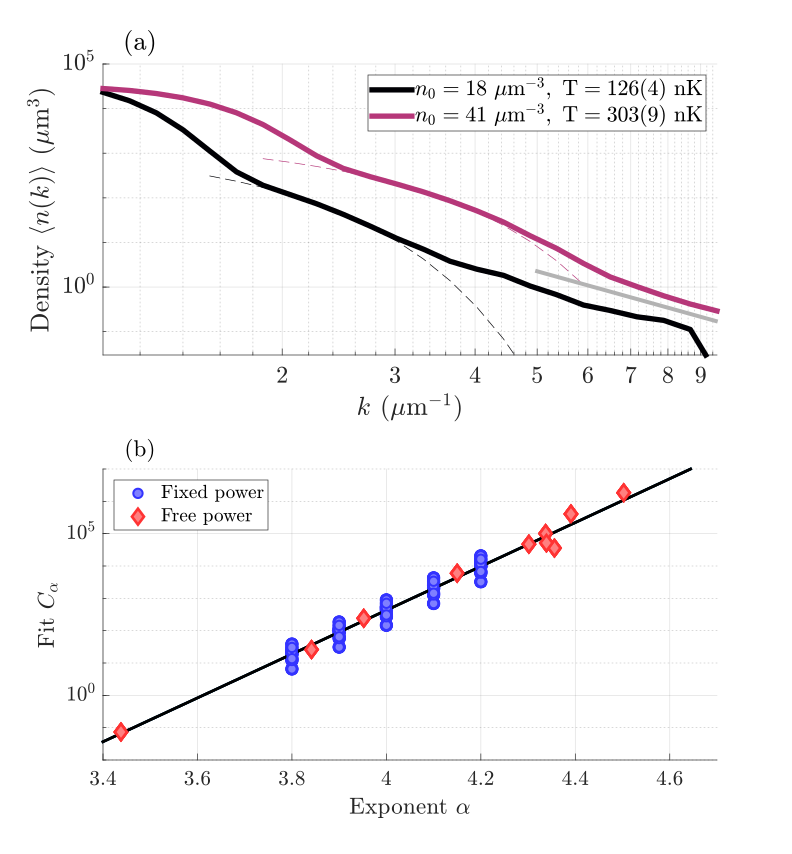
\includegraphics[width=0.5\textwidth]{fig/depletion/exp_density}
	        \caption{The empirical density of particle momenta for two traps (a), where the thermal parts (dashed lines) exponentially decay and give way to the depletion region, marked with grey dashed line proportional to $k^{-4}$.
	        In (b) we illustrate the large hidden systematic errors in a fit to the density which a power law.
	Leaving $\alpha$ as a free parameter gives a wide variation in best-fit exponents and scale coefficients.
	Blue squares show the amplitude coefficient $C_\alpha$ given a fixed exponent $\alpha$ fixed at five values within the range of fit results, applied to all data sets.
	The choice of $\alpha$ powerfully determines the coefficient $C_\alpha$, but the error bars (standard errors in fit parameters) are smaller than the markers in all cases.}
	        \label{fig:contact_determination_issues}
	\end{figure}


	In Fig.
	\ref{fig:contact_determination_issues} (a) we show the empirical density $n(k)$ for two data collection runs at the extreme values of $n_0$ we used.
	The three regimes of the condensate, thermal depletion, and quantum depletion span over five orders of magnitude in density.
	The thermal part of the distribution is well fitted by the momentum distribution of an ideal Bose gas,
	\begin{equation}
		n_T(k) =\frac{N_T}{\zeta(3)} ~\left(\frac{\lambda_{dB}}{2\pi}\right)^3 g_{3/2}\left(\exp\left(-\frac{k^2 \lambda_{dB}^2}{4\pi}\right)\right)
		\label{eqn:th_fun}
	\end{equation}
	wherein the thermal de Broglie wavelength $\lambda_{dB} = \sqrt{2\pi\hbar^2/(m k_B T)}$  yields an estimate of the temperature $T$ which ranges from 100 to 320 nK in our experiments.
	Here, $g_{3/2}(\cdot)$ is the standard Bose integral, $\zeta(\cdot)$ is the Riemann zeta function, and $N_T$ is the number of atoms in the thermal part.
	The thermal population decays exponentially with $k$, and hence cannot account for the counts we observe beyond $k\gtrsim 6~\micron^{-1}$.
	
	In rest of this section we present evidence in support of the identification of these counts with the quantum depletion.
	
	First, though, we show that the otherwise ubiquitous approach of a least-squares regression with a density function is inappropriate in this context.

\subsubsection{Issues with analysis of power laws}	
\label{sec:pow_issues}

	Proceeding with a routine fit of the $k$-space histogram with an additional term of the form $C/k^\alpha$ would appear to be an unobjectionable way to estimate the parameters of the purported quantum-depleted tail.
	However, fitting histograms with power laws is prone to return biased estimates of parameters and to drastically under-report uncertainties, especially when data is available over less than a couple of decades of dynamic range \cite{Clauset09,Virkar14}.
	
	As the authors of \cite{Clauset09} note, ``In practice, we can rarely, if ever, be certain that an observed quantity is drawn from a power-law distribution.
	The most we can say is that our observations are consistent with the hypothesis that $x$ is drawn from [a power law]"
	In this section, we demonstrate some of the problems with a least-squares regression using our data as a case study.
	In the next section we discuss our alternative approach and the inherent limitations of analysing data of this nature.
	
	If we augment the fit function (Eqn.
	(\ref{eqn:th_fun})) with power-law term and leave $\alpha$ as a free parameter, the average exponent of over all runs is 4.2(4).
	
	For comparison, the prior work \cite{Chang16} reported power-law tails with an exponent 4.2(2).
	At first glance, one could simply determine the amplitude of the tails by fixing the exponent to 4, and perhaps achieve better results by using a fit weighting proportional to $k^4$.
	 
	Indeed if we do so, we find an average $C_{\alpha=4}$ which is approximately 8(2) times greater than the coefficient of Eqn.
	(\ref{eqn:pred_scaling}), and in general agreement with ref.
	\cite{Chang16}.
	However, there are issues which undermine the reliability of this otherwise standard approach.

	First, in Fig.
	\ref{fig:contact_determination_issues} (b) we illustrate how the choice of scaling exponent $\alpha$ leads to an exponential change in the scale coefficient $C_\alpha$ that one obtains from fitting to a fixed dataset.
	The coefficient $C_\alpha$ varies over about three orders of magnitude \emph{either way} as one uses different exponents $\alpha$ which lie within the range of uncertainties reported here and in the prior work \cite{Chang16}.
	
	Furthermore, this problem is not reflected in the error estimates in the fitting routines: The error bars representing the uncertainty in fit amplitude are smaller than the markers used in Fig.
	\ref{fig:contact_determination_issues} (b).
	
	A linear fit shows that $d \log_{10} C/d\alpha \approx 6.8$, from which we can infer the exponent that would yield an amplitude in good agreement with Eqn.
	(\ref{eqn:pred_scaling}).
	
	This turns out to be approximately 3.9, which lies within one standard deviation from the mean exponent obtained from the regression we just described.
	
	Conversely, we can estimate that the best-fit exponents reported in the prior work would lead to scale coefficients a factor of about 23 greater than their conclusions, and the associated variance could be even larger.
	It is easy to see that a well-intentioned choice of $\alpha$, which is not statistically different from the best-fit estimates, can lead to  conclusion which either agrees perfectly or disagrees catastrophically with the predictions of Eqn.
	(\ref{eqn:pred_scaling}).
	In particular if one assumes that the data conforms to a power law with $\alpha=4$, one is forced to conclude that the Tan theory is wrong, but the inherent -- hidden -- uncertainty in this approach precludes the possibility of such a definitive statement.


	Second, a deceptively reassuring result can be found by multiplying the empirical density by $k^4$, observing a flat region, and adding a constant term in an appropriately scaled model of the thermal region (i.e.
	Eqn.
	(\ref{eqn:th_fun}) multiplied by $k^4$).
	
	In fact, this offers no recourse from the issues described above and is not a definitive test for the presence of a power law or a way t obtain its parameters.
	Suppose the density decays as some $C k^{-(\alpha+\epsilon)}$: then following the rescaling operation $k^\alpha n(k)$, one then has a density which would be expected to be have the form $C k^{-\epsilon}$.
	
	A variation in the (true) $\alpha$ within the systematic variation above leads difference of a factor of $O(2^{0.1})\approx1.07$ over the range $5\micron^{-1}\lesssim k\lesssim10\micron^{-1}$ range reported here and in \cite{Chang16}.
	This variation is dominated by the statistical fluctuations arising in the individual density profiles from random sampling, and is not distinguishable from the run-to-run variation in the power law.
	
	Despite this, fitting such a weighted distribution is similarly sensitive to the choice of weighting function
	For example, fixing the fit exponent at $\alpha=4$ and changing the \emph{weighting function} (not the form of the fit) in the fit from $k^4$ to $k^{4.1}$ returns a coefficient different by a factor of ten.
	This points to one of the primary challenges with power laws; the exponent are strongly entwined with the rate of occurrence of rare events, which by definition are subject to large statistical errors and thus subvert even the most meticulous investigations.

	In sum, these problems with fitting power laws are ubiquitous, and made more difficult by the small range of $k$ which are visible in the helium experiments.
	In general, estimating the exponent of a purported power law is difficult and requires data spanning several orders of magnitude in scale \cite{Goldstein04,Clauset09,Virkar14,Hanel17}, which are not present in either helium experiment.
	The preferred statistical tools for analysing power law distributions are maximum likelihood estimators, as discussed in lucid terms in Refs.
	\cite{Clauset09,Virkar14}.
	However, in these particle detection experiments the limited sampling region and presence of spurious detection events (described below) mean that such estimators are not appropriate.
	In the next section we describe an alternative approach which does not require -- and conversely cannot determine -- a precise value of the scaling exponent.
	We hope this discussion provides the theoretical and experimental community with an understanding of some problems with heavy-tailed distributions and points the way towards a sound analysis of such phenomena in future works.
	 % which neither assumes the data conforms to the theory under test nor requires precise determination of the exponent of the power law.
	
	
	\begin{figure}[t]
	\begin{center}
		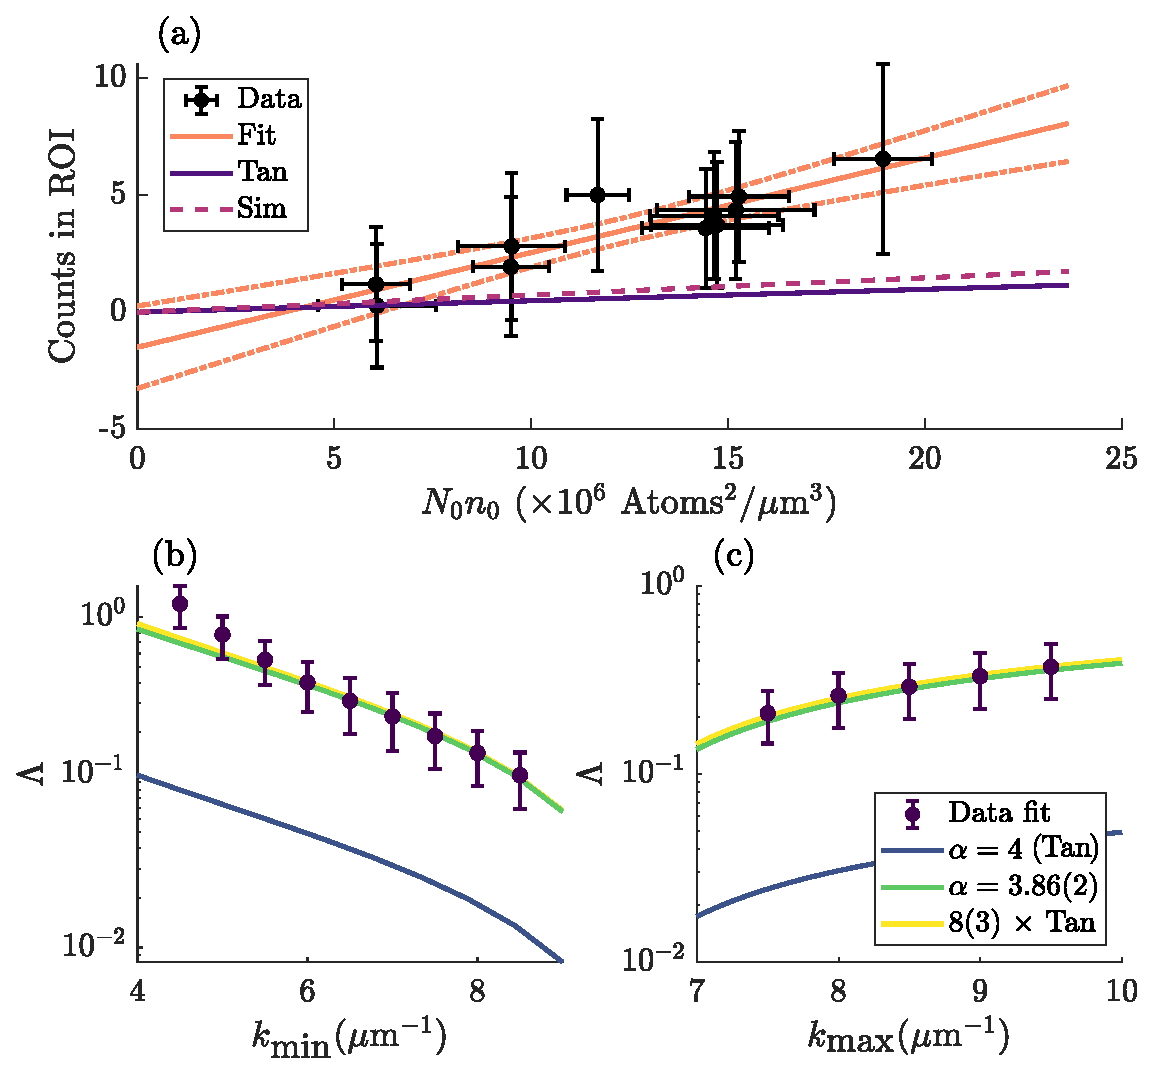
\includegraphics[width=\columnwidth]{fig/depletion/exp_results}
			\caption{A linear fit (a) shows that the product $N_0n_0$ is a good predictor of the number of counts within a region $(k_\textrm{min},k_\textrm{max})$, consistent with Eqn (\ref{eqn:pred_scaling}).
	The gradient $\Lambda_\textrm{fit}$ can be predicted using Eqn (\ref{eqn:pred_scaling}) but the two results disagree by a factor of about 8.
	The number of counts, hence $\Lambda$, depend on the choice of $k$ bounds, as shown in (b,c).
	This dependence does not provide estimates of $C$ or $\alpha$ because multiple hypotheses can produce indistinguishable behavior.
	In (b,c) we show predictions based on Eqn (\ref{eqn:pred_scaling}), along with the predictions of a density function $n(k)$ that is approximately 8(3) times Eqn.
	(\ref{eqn:pred_scaling}) and one that has exactly the amplitude $\mathcal{C}$ but a modified exponent.
	In (b), the deviation from the predictions at $k_\textrm{min}\lesssim6~\micron^{-1}$ is because the collection area starts to overlap with the thermal region.
			}

		\label{fig:exp_results}
	\end{center}
	\end{figure}

\subsubsection{Testing Tan's Tails}

	The prediction of the momentum tail shape (via Eqn.
	(\ref{eqn:pred_scaling})) captures a great deal of information, which can be split into two independently testable hypotheses.
	
	The first claim which we test is that the amplitude of this tail scales in proportion to the product $n_0 N_0$, and the second is the exponent of the density decay.
	Under the null hypothesis that the \emph{in situ} depletion survives the expansion and escapes the condensate undisturbed, one can integrate Eqn.
	(\ref{eqn:pred_scaling}) to predict the number of atoms whose wavevector has a modulus in the interval $k\in (k_\textrm{min}, k_\textrm{max})$, 

	\begin{equation}
		N_{k_\textrm{min},k_\textrm{max}} =\frac{\mathcal{C}}{2\pi^2}\left(\frac{1}{k_\textrm{min}}-\frac{1}{k_\textrm{max}}\right)
		\label{eqn:pred_num}
	\end{equation}
	Note that the integral of $n(k)$ is taken with the differential form $(2\pi^{-3})\d\kvec$ in spherical coordinates.
	For fixed $k_\textrm{min}$ and $k_\textrm{max}$, Eqn.
	(\ref{eqn:pred_num}) has the form $N_{k_\textrm{min},k_\textrm{max}} = \Lambda N_0n_0$ (c.f.
	Eqn.
	\ref{eqn:pred_scaling}).
	
	We can test this form directly by measuring the number of counts detected in the interval $(k_\textrm{min},k_\textrm{max})$ after producing a BEC of $N_0$ atoms with peak density $n_0$.
	
	The figure of merit for this description will be the goodness of fit of a simple linear regression.
	
	As above, we choose $k_\textrm{min}=6~\micron^{-1}$ which lies outside the thermal part for all our data sets.
	However, the $k$-space field of view is restricted by the detector radius to $k\lesssim5\times 10^6$ m$^{-1}$ in the $(x,y)$ plane, which is only just sufficient to reach past the edge of the thermal region.
	
	We thus face a tradeoff in the choice of $k_\textrm{max}$, therefore we define the bounds of our region of interest (ROI) by the minimum elevation angle $\phi_c=\pi/3$ rad and an upper bound of $k_\textrm{max} = 10\micron^{-1}$.
	This amounts to an ROI consisting of two vertically oriented conical sections, each with half-angle $\pi/6$, encompassing a total solid angle of $0.13\times 4\pi$ steradians.
	
	We must also account for the detector quantum efficiency of 0.08(2) and state-transfer efficiency of 25(2)\%, and combine all these factors into the total efficiency $\epsilon\approx0.23(5)\%$.
	After we discuss the results of this analysis, we will  examine the (lack of) effect of uncertainty in $\epsilon$ and the choice of $\phi_c$.
	% We find that the observed number $N_\textrm{exp}$ is 
	% Further, a straight line in a log-log plot is far from conclusive evidence of a power law as there exist other distributions (such as the log-normal and exponential distributions) which also present this way over larger domains than resolved in either of the helium experiments.	
	
	
	% Fixing the power at 3.86 yields 0.8(2) times the predicted contact
%     And at the 95% CI 
%         3.84 0.6(2) times Tan
%         3.88 1.1(3) times Tan
%     But it's not clear what this would mean, physically speaking...
%     so that would be approx 0.8(3) times Tan theor


	A linear fit of the form $\hat{N}_{k_\textrm{min},k_\textrm{max}} = \Lambda_\textrm{fit} n_0 N_0 + c$ yields a vertical intercept $c$ consistent with zero (c=-0.9,  95\% CI (-3.1, 1.2)) and a good correlation ($r^2\approx0.8$, $p=1\times10^{-3}$), providing evidence supporting the expected linear relationship.
	
	The correlation coefficient between the (normalized) variables $N_\textrm{exp}$ and $N_0n_0\propto(N_0^7\bar{\omega}^6)^{1/5}$ is 0.9.
	We conclude that the product $N_0n_0$ is a predictor of the depleted population, which is consistent with Eqn.
	\ref{eqn:pred_scaling}.
	We tested other combinations of the independent variables and found no physically-motivated combination provides a better fit.
	For comparison, a linear fit proves that the atom number itself is a poor predictor of the detected number ($r^2=0.05~,p=0.54$), as is the density alone ($r^2=0.4~,p=0.04$).

	The gradient $\Lambda_\textrm{fit}$ is of particular interest because it can be predicted using Eqn.
	\ref{eqn:pred_num}.
	Given an ROI, one can calculate $\Lambda_\textrm{pred} = 32 \epsilon a^2(k_{\textrm{min}}^{-1}-k_{\textrm{max}}^{-1})/7$.
	We find that the predicted slope disagrees with the empirical fit by a factor of $\Lambda_\textrm{fit}/\Lambda_\textrm{pred}= 8.3$, 95\% CI $(5.5,11)$.


	We are then tasked with reconciling the nonlinear scaling of the detected counts, which is consistent with the quantum depletion, and the disagreement over the absolute number of detected counts.
	We may look to understand the disagreement in terms of the deviation from Eqn.
	(\ref{eqn:pred_scaling}).
	We focus on the two most parsimonious alternatives: whether the tail amplitude is simply larger than expected (i.e.
	$n(k)=A\mathcal{C}/k^4$), or whether the tail decay is somehow modified (i.e.
	$n(k)=\mathcal{C}/k^{4+\delta})$.
	The former would imply that the derivation using the sweep theorem (or Bogoliubov theory in a local density approximation \cite{Chang16}) misses something essential about the system.
	The latter could point to some physical effect, either analogous to the prethermal dynamics of unitary gases \cite{Makotyn14,Eigen18,Colussi20,Kira15_coherent,Smith14} or another factor particular to the dilute regime.
	
	Ultimately, such a distinction between these hypotheses is not possible given the data at hand.
	
	% Specifically, through the appearance of the $k$ boundary values in Eqn.
	\ref{eqn:pred_num}, one could look to the $k$-depndence of $\Lambda_\textrm{pred}$ for a test of the density \emph{ansatze} above.
	Specifically, the density profiles $n(k)=A\mathcal{C}/k^4$ with $A=8(3)$ and $n(k)=\mathcal{C}/k^{\alpha}$ with $\alpha=3.86(2)$ both predict the variation of $\Lambda_{pred}$ with $k_\textrm{min}$ and $k_\textrm{max}$ with comparable accuracy (Fig.
	\ref{fig:exp_results} (b,c)).
	% In other words, if one insists on fitting a distribution of the form $k^{-4}$ then one concludes that the prediction for $\mathcal{C}$ is wrong by a factor of 8(3).
	It is thus not possible to tell whether we have a tail with the expected exponent but a greater weight, or the correct weight but a slower decay, or some combination of the two.
	% Indeed, the space of possible alternative hypotheses is practically infinite: One could find equally-apt distributions by modifying the power and coefficient together.
	Without the ability to precisely determine the exponent $\alpha$, there is insufficient evidence to conclude which of these is correct, therefore little can be said with certainty about which aspect of Eqn.
	(\ref{eqn:pred_scaling}) is incorrect or what physical effects might underpin this disagreement.
	Indeed, the predicted $k^{-4}$ behaviour is only a strict constraint inasmuch as it can be shown to persist (exactly) after the expansion, which as we argued above is not feasible, and argue below is not necessarily expected.
	One conclusion remains robust: There are about ten times as many detections in the depletion region as one would expect based on the Tan theory.
	
	Later in this section we provide technical details of our experiments and rule out several systematic factors which could lead to this disagreement.

	% Although our method provides a direct test of one aspect of Eqn.
	(\ref{eqn:pred_scaling}), it does not circumvent the fundamental challenges of analysing power laws.
	

	Nonetheless, the particular nonlinear scaling of detected counts with the predictor $N_0n_0$ is concordant with the tails' originating in the quantum depletion.
	Furthermore, our simulations indicate that the quantum depletion can survive the condensate expansion, presenting depleted tails in the far-field with modified amplitude.
	
	We are therefore faced with the conclusion that tails are indeed a signature of quantum depletion, albeit subject to some effect during expansion into which the present analysis can see no further.
	Given the similarity in settings and findings, the same could be said for the prior work \cite{Chang16}.
	% Comparing our work to \cite{Chang16}, given the similarity between experiments and consistency of the regression results above, our work can be said to corroborate their findings, albeit withthe prior work appears subject to the same limitations.
	
	
	% Our results could be seen as a count against the interpretation of these tails as a signature of the quantum depletion.
	
	% However, we note two pieces of evidence that give weight to this interpretation.
	
	% First, we are not aware of any other proposed physical effect which exhibits this specific nonlinear scaling relationship with respect to the atom number.
	% Second, we find evidence in our simulations (see below) that the momentum-space signature of the quantum depletion does survive the condensate expansion, and indeed appears in excess of the predicted \emph{in-situ} depletion.
	
	
	


\subsection{Experimental details}
\label{sec:exp_details}
\subsubsection{Trap configuration}

	We prepared our BECs with via forced evaporative cooling in a harmonic magnetic trap with trap frequencies $(45,425,425)$ Hz and a DC bias stabilized by our auxiliary field compensation coils \cite{Dall07,Dedman07}.
	For the tight trap we increased the coil current after the cooling sequence to obtain trapping frequencies $(71,902,895)$ Hz, ramping the field as a sigmoid step function to minimize in-trap oscillations.
	Note that the weak ($x$) axis of the trap is horizontal, with tight vertical confinement.
	The trap remained on for 150ms before switching the trap off with a $1/e$ time of $\approx38\mu$s.
	The condensates were allowed to expand for 2ms before we transferred some of the condensate into the magnetically insensitive $m_J=0$ state via Landau-Zener sweep to prevent distortion by stray magnetic fields.
	The RF pulse was created by a  function generator, amplified, and applied to the experiment chamber by a coiled antenna inserted into the BiQUIC coil housing.
	The pulse swept from 1.6-2.6MHz over 1ms and was centred on the fine structure resonance between the $m_J$ states.
	The determination of the transfer efficiencies $\eta_j$ for each of the $m_J = j$ states is discussed below.
	The sweep was $10^6$-fold wider than the Doppler broadening of the BEC which ensured uniform transfer at all momenta.
	Immediately after the RF sweep, the bias coils are switched off and auxiliary push coils in the vertical (Z) and weak horizontal (X) axes are activated using a fast MOSFET switch to implement a Stern-Gerlach separation of the $m_J = -1,~0,$ and $+1$ pulses.

	We use a Roentdek DLD80 multichannel plate and delay-line detector stack \cite{Manning10} located 859mm below the trap, which registers the arrival times and positions $(t_i,x_i,y_i)$ of each atom, indexed by $i$.
	
	The velocity of each atom relative to the centre of mass of each cloud is calculated by $(v_x,v_y,v_z) = t_{i}^{-1}(x_i-\bar{x},y_i-\bar{y},g_0(\tau^2-t_{i}^{2}))$, where $g_0$ is the local gravitational acceleration and the overbar denotes the within-shot average and $\tau$ ms is the time of flight of the centre of mass of the cloud.
	
	The far-field momentum is thus obtained via $m\textbf{v} = \hbar\kvec$.
	The velocity conversion assumes a point source but carries a negligible error of a few ppm as the in-trap BEC size is smaller than the detector resolution.
	
	The space and time resolution of the detector are 100 $\mu$m and 3 $\mu$s, respectively \cite{Henson18}, and the detector efficiency of $8(2)\%$ was determined from the collection efficiency of correlated atoms on the opposite sides of scattering halos \cite{shin19,shin20,Jaskula10}.
	

	\com{While the determination of the factor $\epsilon$ is important, the dominant uncertainty is the 25\% error in the detector efficiency.
	The collection area cutoff $\phi_c$ also factors in but this is precisely known.
	
	We performed the analysis described above for a range of $\phi_c$ and values of the QE and found that the excess of counts (expressed as $\Lambda_\textrm{fit}/\Lambda_\textrm{pred}$) was not significantly effected, which we summarize in Tab.
	\ref{tab:choice_indep}.}

	\begin{table}[b]
		\begin{tabular}{c c c c}
			\hline\hline
			% $k$ lim.
	($\micron^{-1}$) & fit $r^2$ &  $\Lambda_\textrm{fit}$ & $\Lambda_\textrm{fit}/\Lambda_\textrm{pred}$\\  
			% \hline
			% (6,7)  &  0.88     & 0.2(0.1,0.2) &   9.1(6.5,11.7)\\
			% (6,8)  &  0.85     & 0.3(0.2,0.3) &   8.4(5.7,11.1)\\
			% (6,9)  &  0.83     & 0.3(0.2,0.4) &   8.1(5.3,10.8)\\
			% (7,10)  &   0.79     & 0.2(0.2,0.3) &   7.8(4.8,10.8)\\
			% (8,10)  &   0.79     & 0.1(0.1,0.2) &   8.0(4.9,11.2)\\
			% \hline
			QE & fit $r^2$ &  $\Lambda_\textrm{fit}$ & $\Lambda_\textrm{fit}/\Lambda_\textrm{pred}$\\      
			\hline
			0.05    &   0.83   &   0.2(0.1,0.3)  &  6.8(4.5,9.1)\\
			0.06    &   0.83   &   0.3(0.2,0.4)  &  7.4(4.9,9.8)\\
			0.07    &   0.83   &   0.3(0.2,0.4)  &  7.8(5.2,10.5)\\
			0.08    &   0.83   &   0.4(0.3,0.5)  &  8.3(5.5,11)\\
			0.09    &   0.83   &   0.5(0.3,0.6)  &  8.7(5.8,11.6)\\
			0.1     &   0.83   &   0.6(0.4,0.7)  &  9.0(6.0,12.1)\\
			0.11    &   0.83   &   0.6(0.4,0.8)  &  9.4(6.2,12.5)\\
			\hline
			Half-angle & fit $r^2$ &  $\Lambda_\textrm{fit}$ & $\Lambda_\textrm{fit}/\Lambda_\textrm{pred}$\\
			\hline
			10$^\circ$    &   0.82   &   0.1(0.0,0.1) &  9.3(6.0,12.7)\\
			20$^\circ$    &   0.86   &   0.2(0.1,0.3) &  9.2(6.4,12)\\
			30$^\circ$    &   0.83   &   0.4(0.3,0.5) &  8.3(5.5,11)\\
			\hline\hline
		\end{tabular}
		\caption{The uncertainty in the detector quantum efficiency (QE) does not have a significant effect on the findings.
	Re-running the analysis using different QE yields fits that barely differ in the goodness of whose gradients do not significantly change.
	We also find that the choice of collection area has a weak effect, below statistical significance, on the result.
	Terms in brackets are the upper and lower 95\% confidence intervals.}
		\label{tab:choice_indep}
	\end{table}
	 % we show in Tab.
	\ref{tab:choice_indep}, this has no significant effect on the conclusion (namely, on the comparison $\Lambda_\textrm{fit}/\Lambda_\textrm{pred}$)
	% This could affect the outcome in two ways, first by changing the value of $\chi$ used in the prediction, and second through the factor of $N_{0}^7/5$ used to compute the condensate density $n_0$.
	



\subsubsection{Peak density calibration}

    The quantum depletion and contact are both predicted to depend solely on the condensed number and trapping frequencies via the condensate density, hence it is important to determine both quantities accurately.
	
    % In the Thomas-Fermi approximation, the peak density of the condensate can be written as $n_0 = \mu/g$, where $\mu$ is the chemical potential, $g=4\pi\hbar^2a_{1,1}/m$ is the effective interaction strength, $m\approx6.6\times10^{-27}$ kg is the atomic mass, and $a=7.512$ nm is the s-wave scattering length between pairs of atoms in the $m_J=1$ state \cite{Moal06}.
	
    The sole experimental parameters in the expression for the peak density (Eqn.
	\ref{eqn:n0}) are the geometric trap frequency $\bar{\omega} = \left(\omega_x\cdot\omega_y\cdot\omega_z\right)^{1/3}$, and $N_0$, the number of atoms in the condensate.
	
    We simultaneously determine the total atom number $N$ and trap frequency $\bar{\omega}$ in a single shot using a pulsed atom laser and use the thermal fraction (as below) to determine the condensed number $N_0$.
	

	The pulsed atom laser consists of a series of Fourier-broadened RF pulses centred on the minimum Zeeman splitting in the trap.
	
	The pulse transfers atoms in the trap to the untrapped $m_J=0$ state with an approximately constant transfer rate across the cloud.
	
	We outcouple approximately 2\% of the atoms per 100$\mu$s pulse for $\approx$200 pulses, which eventually depletes the entire trap.
	
	The atom laser thus prevents the detector from saturating and allows an accurate determination of the atom number, up to a factor of the quantum efficiency.
	
	We determine the trapping frequencies by inducing centre-of-mass oscillations with a magnetic impulse, and find the oscillation period from the atom laser pulses \cite{henson18ML}.


\subsubsection{Determining spin transfer efficiency}

	To calibrate the transfer efficiencies, we applied a weaker Stern-Gerlach than for the depletion measurement, resolving each $m_J$ cloud on the detector, as illustrated in Fig.
	\ref{fig:frac_cal}.
	

	\begin{figure}[!t]
	\begin{center}
		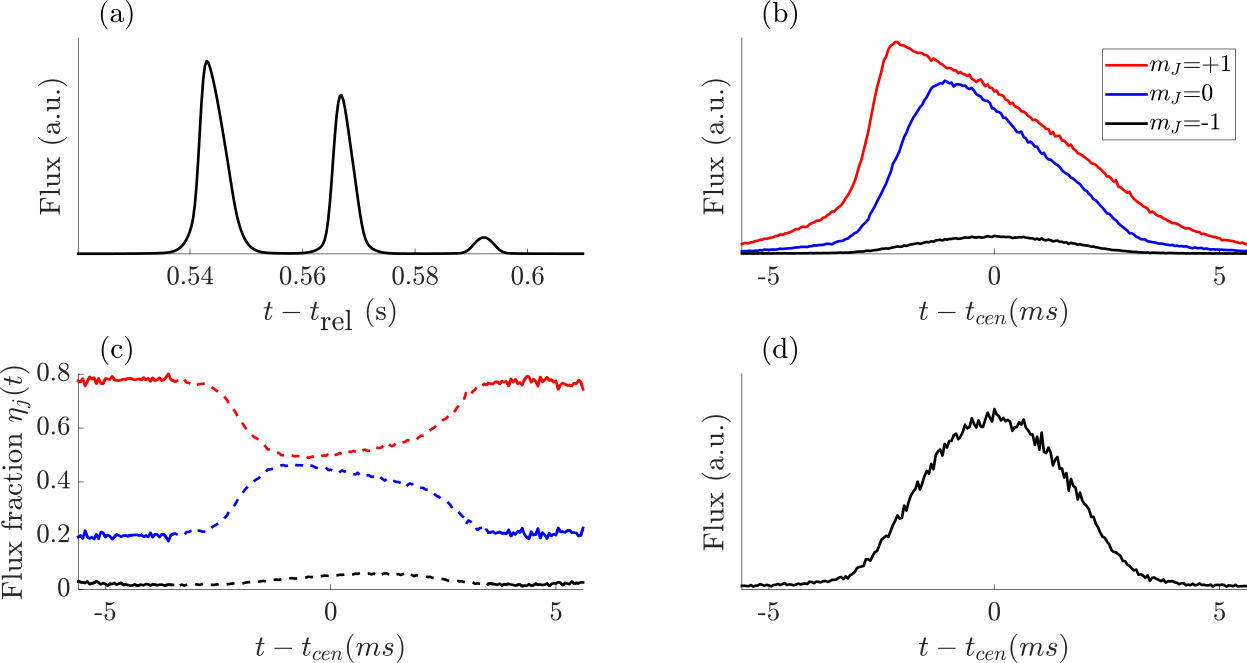
\includegraphics[width=\columnwidth]{fig/depletion/frac_cal_profile}
		\caption{Determining the RF transfer efficiency.
	The time-of-flight profiles of each pulse are resolved (a) by applying a weak Stern-Gerlach pulse during the time of flight.
	The pulses are aligned with respect their centre-of-mass (b) and used to determine the pointwise fraction ((c), dotted line).
	Detector saturation is evident in the peaks (dashed lines), but not in the thermal tails (solid lines), which are used to compute the transfer efficiency.
	Because of its lower flux, the $m_J=-1$ pulse does not show evidence of saturation (d) and is used to determine the thermal fraction.}
		\label{fig:frac_cal}
	\end{center}
	\end{figure}

	The efficiencies $\eta_J$ cannot be calculated by counting the atoms in each cloud because the detector saturates during the peak condensate flux, but we can compare the thermal parts.
	
	We align each cloud along the time (Z) axis and compute the pointwise fraction of the atomic flux $\phi(t)$ accounted for by each cloud, $\eta_j(t) = \phi_j(t)/\sum_j\phi_j(t)$, as depicted in Fig.
	\ref{fig:frac_cal}.
	
	The ratio of densities between the clouds is roughly constant in the thermal part, indicating the absence of important saturation effects and a spin transfer that is independent of $k$.
	
	The fraction of the original cloud transferred into each $m_J$ state is determined by taking the average $\langle\eta_j(t)\rangle$ over the thermal tails.
	
	We find these efficiencies are approximately 74\%, 24\%, and 2\% in all runs for the $m_J=+1$, 0, and -1 states, respectively.
	
	While the $m_J=0$ and $m_J=1$ clouds clearly saturate the detector, the small fraction ($\approx2\%$) of the atoms transferred to the $m_J=-1$ state does not (Fig.
	\ref{fig:frac_cal} (d)).
	
	A bimodal fit to the condensed and thermal parts, plus constant background, yields the thermal and condensed fractions.

	% \com{After a 2ms expansion the cloud is even more dilute than the trap, with a peak density that has approximately halved.
	Therefore the Because the contact in a mixed-species condensate \cite{Vassen16,Werner12_boson}, even if the condensate were still as dense as the in-trap distribution, the contact is reduced relative to the spin-polarized condensate.
	Considering also the reduced density after 2ms expansion, the production rate of quantum-depleted quasiparticles is expected to \emph{decrease} during this process, hence the observed effect is unlikely to emerge at this stage.}
	

% \subsection{Determination of thermal fraction}
	

% 	\begin{figure}[!h]
% 	\begin{center}
% 		\includegraphics[width=0.8\textwidth]{fig/depletion/m1_frac_anal}
% 		\caption{Comparison of thermal fits in the unsaturated $m_J=-1$ pulse including 138 shots.
	The weak (X) and strong horizontal (Y) trapping axes are shown in (a) and (b), respectively.
	\org{would be helpful to label $v_x$ and $v_y$ to make it self-evident at 1st glance.} Both projections display a bimodal peak, with the condensate (dotted lines) and thermal parts (thick solid lines) easily distinguished.
	Fitting a Gaussian profile (thin solid line) to the velocity distribution of the thermal part yields the thermal number and temperature.
	Subtracting the fit leaves the condensate profile (c) which can be \blu{\dots something\dots} yields the condensed number.}
% 		\label{fig:thermal_frac}
% 	\end{center}
% 	\end{figure}


\subsubsection{Noise sources}
\label{sec:spinpop}

	In early tests of our measurement sequence we noticed a contamination of the signal by spurious counts.
	
	We inferred these were remnant counts from the $m_J=+1$ cloud as they were still visible when we ran an experimental sequence without the Landau-Zener transfer.
	
	This contamination appeared in a particular region of our detection image, and as such we were able to correct for it by subtracting their contribution from the counts collected during measurement shots.
	
	Generally, fewer atoms can be attributed to this noise than would be required to explain the discrepancy described in the main text.
	
	While the cause of the cross-contamination is unclear, we observe that the count density outside the region of interest is similar in both the shots with the RF pulse and those without.
	
	We hypothesize that the remnant counts are atoms transferred into the $m_J=0$ state by non-ideal behaviour of the Stern-Gerlach pulses.
	
	We note that only about one in a million atoms from the $m_J=1$ cloud present in this manner in a given shot.

	\com{Such counts constitute about 10(5)\% of the detection events in the ROI.
	Because it is not possible to distinguish \emph{which} atoms are spurious and which are genuine quantum-depleted particles, the preferred power-law analysis (the maximum-likelihood estimator) is not available.
	Basic MLEs are built assuming one has a sample drawn from a distribution of a single category; the probabilistic combination of two different sources of events falls outside the scope of this framework.}


% \begin{table}
% 		\begin{tabular}{ccccccc}
% 		\hline \hline 
% 		$n_0$ ($\mu$m$^{-3}$)  & $N_0\times10^{-5}$ & $\eta_\textrm{Th}$ & T (nK) & $N_\textrm{det}$ & $N_\textrm{pred}$ & $N_\textrm{det}/N_\textrm{pred}$ \\ 
% 		\hline 
% 		17(2) & 3.6(3) & 0.09 & 130(20) & 1.2(1) & 0.3(1) & 5(2) \\ 
% 		17(3) & 3.6(6) & 0.08 & 190(20) & 0.3(04) & 0.3(1) & 1(1) \\ 
% 		19(1) & 5.1(3) & 0.18 & 150(10) & 1.9(1) & 0.3(1) & 6(3) \\ 
% 		19(2) & 4.9(5) & 0.09 & 150(10) & 2.8(1) & 0.4(1) & 7(4) \\ 
% 		20(1) & 5.7(2) & 0.1  & 137(9)  & 5.0(1) & 0.5(1) & 10(4) \\ 
% 		39(4) & 3.8(3) & 0.11 & 252(3)  & 3.7(1) & 0.6(1) & 6(4) \\ 
% 		39(4) & 3.9(3) & 0.11 & 268(2)  & 4.4(1) & 0.6(1) & 8(5) \\ 
% 		39(3) & 3.8(3) & 0.1  & 249(3)  & 4.1(1) & 0.5(1) & 8(4) \\ 
% 		39(3) & 3.7(3) & 0.09 & 237(3)  & 3.6(1) & 0.5(1) & 7(4) \\ 
% 		39(3) & 4.0(2) & 0.14 & 312(3)  & 4.9(1) & 0.5(1) & 10(5) \\ 
% 		41(2) & 4.6(2) & 0.12 & 302(3)  & 6.6(2) & 0.7(2) & 10(6) \\ 
% 		\hline \hline 
% 		\end{tabular}
% 		\caption{Summary of results for each data run.
	The peak density is determined from measurements of the trapping frequencies and the condensed number (via $N_0=N_\textrm{tot}(1-\eta_\textrm{Th})$, using the total number $N_\textrm{tot}$ and thermal fraction $\eta_\textrm{Th}$).
	The number $N_\textrm{Detect}$ of atoms detected in the region of interest (results shown here for the largest ROI) can be compared to the predictions of the Tan theory, as in the main text.}
% 		\label{tab:run_results}
% 	\end{table}

	


	

% \subsubsection{Barriers to employing MLEs}

% 	The presence of these counts is one factor preventing a straightforward application of a maximum-likelihood estimator (MLE) to determine parameters of the power-law region.
	
% 	The basic principle of the MLE is to assume a functional form for the probability distribution $p(x|\theta)$ underlying the observed data $x$, and dependent on some parameters $\theta$.
% 	The zero of the derivative of the \emph{likelihood} function $L(\theta|x)$ with respect to the parameters $\theta$ then yields the most-probable parameter values given a set of observations $x$.
	
% 	In our context, one can assume a functional form for the probability distribution underlying atomic detection events (via a wavefunction ansatz).
	
% 	The detector dark counts can also be incorporated by assuming a uniform distribution, although this entails a cumbersome procedure to retain proper normalization.
% 	However, the dark counts present less than one detection per shot, on average, and thus might be ignorable without major consequence.
% 	The major obstacle to implementing an MLE is the finite detection region.
	
% 	Specifically, because the normalization condition 
	

%     \begin{figure}[!b]
% 	\begin{center}
% 		\includegraphics[width=\columnwidth]{fig/depletion/spinpop}
% 		\caption{Measured contribution of the detector dark counts and spurious spin counts to the time-of-flight profile.
% 	We accounted for the pulse at around 550ms and subtracted it from the measured profiles when computing the contact.
% 	After removing this background term, the density profiles above and below the condensate agree, indicating convergence on the true signal.
% 	For reference, the peak flux of the $m_J=0$ condensate is about a thousandfold greater than the peak shown here.}
% % 		\label{fig:spinpop}
% % 	\end{center}
% % 	\end{figure}

% % 	\begin{figure}[!h]
% % 	\begin{center}
% % 		\includegraphics[width=\textwidth]{fig/depletion/profile_overlay}
% % 		\caption{Comparison of average time-of-flight profiles over a single data run for the quantum depletion measurement shots (blue, 871 shots), transfer efficiency calibration (black, 112 shots), detector dark counts (red, 871 shots), and spurious counts (dot-dash, 895 shots).
% 	The time window bounded by $|k|\leq 10\mu$m is indicated with dotted lines.
% 	Shaded area is the standard error over the entire run.}
% % 		\label{fig:tof_profile}
% % 	\end{center}
% % 	\end{figure}




% % Note that the temps disagree between axes, but within axes between clouds they are consistent(....ish).
% 	This means we can use the profile ratio method, which is also consistent with comparing the thermal number from the fits.
% % Perhaps comment on the thermal-subtracted part; the TF profile should have a sharp cutoff, but the smooth edges are suggestive evidence of this roll-off

% % \begin{figure}
% % 	\centering
% % 	\includegraphics[width=0.5\textwidth]{fig/depletion/counts_per_run}
% % 	\caption{Number of counts detected in the region of interest in the depletion measurement (a), the spin mixing calibration (b), and the dark count calibration (c).
% 	An average of 3.0(5) counts were detected in the ROI in the spin-mixing calibration shot, and the background count rate was 0.4(2) counts per shot.
% 	Separate lines indicate separate \emph{runs}, i.e.
% 	sequences of shots with fixed parameters.}
% % 	\label{fig:num_counts}
% % \end{figure}








\section{Numerical simulations}
\label{STAB}
	\begin{figure}[b]
	        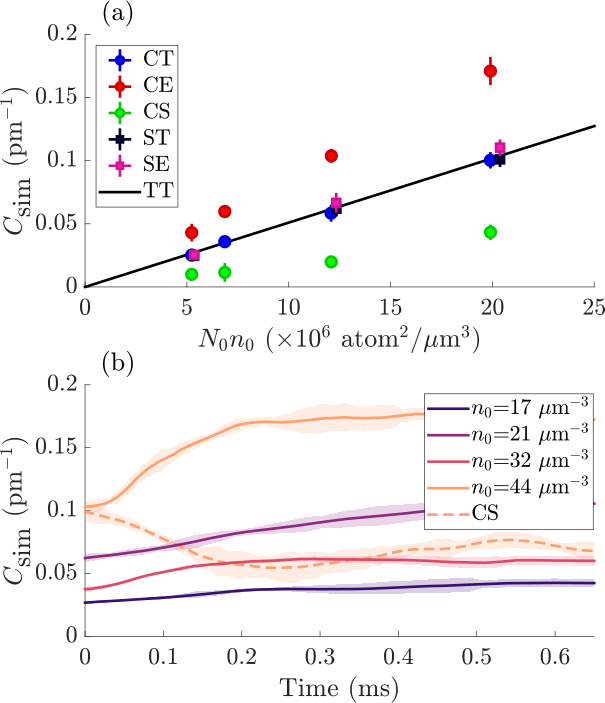
\includegraphics[width=\columnwidth]{fig/depletion/sim_results}
	        \caption{(a) Steady-state values of the simulated contact.
	Simulations of condensates released from a cigar-shaped trap (CT) are consistent with the Tan theory (TT) before release, and show an increase in contact after the trap release (CE).
	A slow relaxation of the transverse trapping frequencies (CS) shows a decrease in line with the predicted value of the lower density.
	Spherical traps (ST,SE) lack any directions of tight confinement, wherein a longer interaction time prevents the escape of depleted particles as seen in cigar traps.
	(b) the time-dependence of the contact stabilizes after a time on the order of $1/\omega_x$, several hundred $\mu$s.
	The difference between in-trap and expanded contact increases with the density of the condensate but is consistently about 1.7 times the Tan theory.
	For comparison, the experimental control pulses are implemented after 2ms of expansion.
	When the transverse trapping frequencies are reduced by half (dotted line), the in-situ contact relaxes.}
	        \label{fig:sim_fig}
	\end{figure}
	We performed simulations of the BEC expansion from harmonic traps using the first principles STAB method \cite{Deuar11,Kheruntsyan12}.
	
	The simulations included a cigar-shaped trap (marked CT in Fig.
	\ref{fig:sim_fig}) with parameters matched to the experimental conditions.
	
	The in-trap state was consistent with the adiabatic sweep theorem before release from the trap.
	
	Following expansion from the cigar trap (CE in Fig.
	\ref{fig:sim_fig})), the simulated tail amplitude increased and stabilized within a few hundred microseconds, much sooner than the 2ms delay between the trap release and application of the rf and Stern-Gerlach pulses.
	
	Fig.
	\ref{fig:sim_fig} shows time evolution of the tail amplitude for the simulated traps using the same ROI as the experimental setup.
	 
	In this configuration the steady-state value of the momentum tails was a factor of 1.64(9) above the predictions of Eqn.
	(\ref{eqn:pred_scaling}).
	

	To understand the disagreement with earlier theory \cite{Qu16}, which predicted no depletion survival, we also investigated the effect of adiabatic expansion on the in-trap depletion by simulating a slow decrease of the transverse trapping frequencies by a factor of two (CS), and found that the in-trap contact decreased roughly as predicted by Eqn.
	(\ref{eqn:pred_scaling}) in these instances --- see the dashed line in Fig.~\ref{fig:sim_fig}.
	
	We also found that the factor of disagreement (i.e.
	$C_\textrm{sim}/C_\textrm{Tan}$) between Eqn.
	(\ref{eqn:pred_num}) and the simulated tails depends on the angle choice of cutoff angle $\phi_c$.
	
	Put another way, the momentum distribution in the simulations is anisotropic and takes the form $f(\theta,\phi)/k^4$ - note that the average of an angle-dependent power law decay preserves the power-law behaviour.
	We find that $C_\textrm{sim}$ is larger for smaller collection regions that are more tightly concentrated about the vertical (strong) trapping axis, whereas larger collection angles (including areas closer to the weak axis) produce a lower $C_\textrm{sim}$.
	In particular, with cone half-angles of 10, 20, and 30 degrees, $C_\textrm{sim}$ was 2.2(3), 1.9(2), and 1.6(1) times $C_\textrm{Tan}$, respectively.
	We note that the experimental results (Tab.
	\ref{tab:choice_indep}) could be said to display a similar trend, but the result is not statisically significant.
	The implementation of the simulations is discussed in detail in the publication \cite{Ross21}.


\section{Discussion}
\label{sec:discussion}

	In sum, we find that the number of atoms in the large-$k$ tails is predicted by the product $N_0n_0\propto(N_{0}^7\bar{\omega}^6)^{1/5}$, in line with Tan's theory of the contact (Eqns.
	\ref{eqn:pred_scaling},\ref{eqn:pred_num}).
	
	However, the sensitivity of this relationship is significantly different than expected by a factor of order 8(3), which is not accounted for by any known systematic effects.
	The method we employ makes a clear distinction between what can and cannot be inferred about the form of the momentum tails, and indeed we find there is no decisive evidence in favour of tails that decay with $k^{-4}$.
	We do note that the prior work \cite{Chang16} reported results which fall within the uncertainty range of our analysis.
	Indeed, Fig.
	4 in \cite{Chang16} could be said to display the relevant scaling with respect to $N_0n_0$ but the reported values of the apparent contact should be considered along with the caveats discussed in Section \ref{sec:pow_issues}.
	
	Taken together with the simulations, our findings show that the survival of the quantum depletion into the far-field is plausible, but not as a straightforward mapping into the far-field density.
	In a non-interacting ballistic expansion, the far-field density distribution would be a direct realization of the in-trap momentum distribution of the cloud.
	
	However, this correspondence is known not to faithful because the dispersal of the mean-field energy into kinetic energy, known as the release energy, imparts some acceleration to the atoms during early expansion.
	
	This effect is responsible for the famous inversion of the cloud aspect ratio upon release from harmonic traps.
	

	As such we interpret our results as an indication that the depleted atoms are accelerated by the non-uniform mean-field energy of the condensate during the expansion.
	In detail, after a quench into the free particle regime, the condensate expands hydrodynamically on timescales of $1/\omega$.
	
	This is an adiabatic process for the low momentum depletion, whereby some depleted atoms are absorbed back into the condensate in agreement with \cite{Qu16}.
	However, the characteristic time for reabsorption is $\hbar/gn_0$, slow enough that quasiparticles in the particle branch of the Bogoliubov dispersion have sufficient velocity to escape the expanding cloud without being reabsorbed and thus transition to free atoms.
	
	This effect leads to the persistence of populated high-$k$ modes in the far-field, which were detected in the experiment.

	Moreover, an atom inside the BEC experiences an effective force from the gradient of the mean-field potential $\textbf{F} = -4\pi\hbar^2 m^{-1}a \nabla  n(x)$.
	
	This endows escaping depleted particles with a greater momentum, increasing the weight of the tails in the far-field.
	
	This effect is exacerbated in light atoms like $^{4}$He, whereas it would be suppressed by a $\sim500$-fold in $^{87}$Rb experiments \cite{Makotyn14} because the acceleration scales with $1/m^2$.
	
	Further, it is much easier for depletion atoms to escape and be accelerated in the transverse x-y directions from an elongated cloud because the distances $R_{TF}=\frac{1}{\omega}\sqrt{2gn_0/m}$ are reduced by $\bar{\omega}/\omega_{x,y}$, whereas the initial mean depletion velocities \textit{in situ} $v\sim \sqrt{2gn_0/m}$ are isotropic.
	Indeed, spherical clouds (SE) exhibit a much weaker effect than the elongated clouds (CE) owing to the longer escape time.
	This also presents as an increase in $C_\textrm{sim}$ for smaller collection regions.
	
	The statistical uncertainty in the experimental findings preclude a definitive comparison on this particular point.

	The interpretation just described is supported by another observation within the simulations:
	During the expansion we observe a decrease in the total number of depleted particles (reabsorption) and a simultaneous increase of the large-k population (forcing).
	
	This constitutes a partial explanation of the experimenal findings too, and results in tail amplitudes which are consistent with the quantum depletion multiplied by a constant factor.
	
	However, a mystery remains: Why is there an excess of particles in the depletion region which is so much greater than accounted for by this picture? 
	This issue should be resolved if far-field observations are to be interpreted in terms of the in-trap physics of interest.
	
	
	As we discussed, our systematic uncertainties are unable to account for the observed excess population of the quantum-depleted tails.
	Futher, despite the ultracold clouds being realized at finite temperatures, the thermal population of quasiparticles cannot account for the observed counts.
	
	The thermal quasiparticles in the Bogoliubov picture simply reflect a change of basis which maps identically onto the thermal population of constituent particles \footnote{See, for example, \cite{PethickSmith} Chap.
	8.3.}.
	
	Quasiparticles whose wavenumber exceeds that of the speed of sound lie within the particle-like branch of the bogoliubov spectrum, which for our considerations is on the order of $k\gtrsim2~\micron^{-1}$, well within the thermal velocities.
	
	Hence, given the exponential decay of thermally populated states, the large-$k$ tails are unambiguously \emph{not} thermal effects.
	

	In conclusion, our work expands the growing suite of far-field investigations of quantum depletion \cite{Cayla20,Chang16} and confirms that quantum depletion can, remarkably, survive past the lifetime of its original condensate.
	
	Our simulations clarify how the depletion can be visible in the far-field momentum distribution here and in earlier experiments, and that the hydrodynamic approximation does not capture sufficient short-wavelength information to make detailed predictions about the high-momentum behaviour.
	
	We thus find a partial explanation for the deviation of the far-field distribution from both the predicted in-situ depletion and the hydrodynamic reabsorption: The interplay between coherent absorption of Bogoliubov excitations and the dispersal of the chemical potential into kinetic energy, to which helium is particularly sensitive, result in a growth of the $k^{-4}$ tails of the momentum distribution during freefall.
	

	It would be informative to determine whether the outstanding discrepancy originates in the trapped condensate or is due to some unknown non-equilibrium effect during expansion.
	This question invites complementary studies of the \emph{in situ} depletion in \mhe BECs.
	
	Such an investigation requires an \emph{in situ} probe of the contact, such as RF spectroscopy or Bragg spectroscopy.
	The latter may be the most fruitful of the two simply because of the difficulty of interpreting the results from the former, which we sketch here.
	
	
	The basic principle of RF contact spectroscopy is to apply a monochromatic RF probe which is detuned from the resonance between two spin states, coupling atoms in the initial spin state to an untrapped channel.
	
	One then performs a differential measurement of the atom number and expects the signal strength to scale as $\omega_\textrm{RF}^{3/2}$ with the detuning from the RF resonance.
	The loss rate is also proportional to the difference of reciprocal scattering lengths $\Gamma\propto(1/a_\textrm{i,i}-1/a_\textrm{i,f})$ between pairs of atoms in initial-initial ($a_{i,i}$) and initial-final ($a_{i,f}$) spin states \cite{Braaten10,Wild12}.
	
	For He$^*$ (spin 1) the scattering lengths $a_{1,1}$ and $a_{1,0}$ are identical \cite{Leo01}, rendering the preferred $m_J=1-m_J=0$ transition unusable.
	
	On the other hand, $a_{1,-1} = 3/7 a_{1,1}$ \cite{Vassen16}, and the singlet transition can be driven without populating the $m_J=0$ state.
	
	In principle this could produce a detectable flux of atoms to perform sensitive in-trap contact measurements, however, collisions in the $^1\Sigma_{g}^{+}$ channel have large Penning ionization rates which lead to significant trap losses \cite{Leo01}.
	
	The ionization products would be detectable by in-vacuum channel electron multipliers but require theoretical work to disentangle from the spectroscopic signal.
	
	Further, while other atomic species offer Feshbach resonances by which to tune the inter-species scattering length (and hence signal or ionization rate), \mhe has no such feature.
	
	While such a measurement is not \emph{prima facie} impossible, Bragg spectroscopy may yield more readily interpretable results.



% \begin{abstract}

% Measurements of Tan's contact in expanding condensate conflict with predictions of the \emph{in situ} quantum depletion.
	% It is unclear how the depletion survives without a condensate, and even appears stronger in the far-field than before the trap release.
	% We confirm experimental observations of a slowly-decaying tails in the far-field, consistent with the survival of the quantum depletion.
	% Simulations of our experiment support shed light on the mechanisms behind the observations.
	% A gap between the numerical and empirical results remains an open question obstructing studies of quantum depletion in the far field.
% % max 600chars for PRL
% % \end{abstract}

% % \maketitle

% \section{Introduction} 
% 	The mechanism underlying superfluid formation is the Bose-Einstein condensation of collective excitations.
	
% 	This was formalized by Bogoliubov’s transformation \cite{Bogolubov47} of a homogeneous system of interacting bosons into a free Bose gas of collective excitations constituted by oppositely-moving particles \cite{Vogels02}.
	
% 	In a superfluid, the macroscopically-occupied quasiparticle ground state corresponds to the superfluid part, and population of excited quasiparticle modes constitute the normal component of the fluid.
	
% 	This foundational theory is of broad relevance because the BEC and BCS regimes of superconductivity are characterized by superfluids of molecular dimers and of Cooper pairs, respectively.
	  

% 	Interactions between constituent particles lead to a zero-point population of quasiparticle modes, known as the quantum depletion, which persists even at zero temperature.
	
% 	The quantum depletion presents as an occupation of single particle modes with large momentum $p$ that decays like $p^{-4}$.
% 	In liquid helium, the depleted fraction is large (of order 90\% of the fluid) due to the strong interparticle interactions, but is generally very small in weakly-interacting dilute gases.
% 	Bogoliubov's theory makes accurate predictions of the total depleted population in ultracold atomic Bose-Einstein condensates (BECs) \cite{xu06,lopes17_depletion} and exciton-polariton condensates in solid substrates \cite{pieczarka20}.
% 	Therefore, detailed study of the quantum-depleted tails of the momentum distribution in ultracold gases is an attractive test for the Bogoliubov theory.

% 	This has been challenging to date because the tails are usually beneath the noise floor of optical imaging techniques.
	
% 	A previous experiment \cite{makotyn14} sought to use a Feshbach resonance to produce a visible depleted fraction, but found that the momentum distribution saturated during expansion and did not display a power-law tail.
	
% 	% \com{This was because complex three-body effects play an important role in the pre-thermalization dynamics, and so the asymptotic momentum distribution is no longer characterized purely by two-body dynamics.
	% \cite{kira15_hyperbolic,kira15_coherent}}
% 	In contrast, another experiment found unexpectedly large momentum tails in the far-field of a weakly interacting helium BEC released from a harmonic optical trap \cite{chang16}.
	
% 	This is particularly surprising because conventional wisdom argues that the density decreases adiabatically during expansion, justifying treatment with a hydrodynamic approximation wherein the tails are predicted to vanish \cite{qu16}.
	

% 	These observations are also in conflict with anither successful and widely applicable theory of contact interactions developed by Tan \cite{tan08_energetics,tan08_momentum,tan08_virial}.
% 	The thermodynamic quantity called the \emph{contact} characterizes how s-wave contact interactions modify the short-range pair correlation function.
	
% 	A defining feature of the contact is that it determines the amplitude of the power-law decay of the momentum density in terms of the gas density and s-wave scattering length, which fully determine collisional dynamics in ultracold dilute gases.
	
% 	Two central properties of the contact, known as the adiabatic sweep theorem and generalized virial theorem \cite{tan08_momentum,tan08_virial}, have been verified via radio spectroscopy \cite{baym07,punk07,braaten10} of degenerate Bose \cite{wild12} and Fermi gases \cite{stewart10,sagi12}.
	
% 	While the Bogoliubov prescription breaks down in strongly-correlated systems \cite{lopes17_quasiparticle}, Tan’s theory applies for arbitrary spin mixtures at any density, temperature, and geometry, and both theories are consistent in the weakly interacting regime.

% 	Thus, it is surprising that the prior work observed such strong tails as this contravenes both the Tan and Bogoliubov theories in the weakly-interacting regime where both have otherwise been demonstrated to be accurate.
% 	This implies that either some feature of harmonically trapped helium condensates violate the minimal assumptions of both theories, or that far-field momentum measurements are not a straightforward means of examining the quantum depletion even in weakly interacting gases.
	
% 	It is important to verify and overcome this obstacle, as far-field measurements play a central role in study of ultracold gases.
	

% 	To this end, we revisit the measurement of the momentum distribution of a helium condensate expanding from a harmonic trap.
	
% 	We conducted experiments using a different apparatus and analysis, covering a range of densities twice as large as the prior work, and use a magnetic trap in place of an optical dipole trap which ensures perfect spin-polarization of the condensate.
	
% 	We observe tails in the large-momentum part of the condensate wavefunction which exhibit a $p^{-4}$-like scaling, and whose amplitude scales in proportion to the condensate population in a manner consistent with the Tan and Bogoliubov theories.
	% However, the absolute amplitude significantly exceeds the predictions of the in situ depletion by a constant factor, corroborating the prior work.
	

% 	Our measurements are complemented by simulations of the time-dependence of the momentum distribution using a stochastic Time-Adaptive Bogoliubov (STAB) method in the positive-P framework \cite{Deuar11,Kheruntsyan12}.
	
% 	These show that the non-adiabatic release of the trap is responsible for survival of the depletion, and that the depleted particles acquire additional kinetic energy from the mean-field energy of the condensate during the subsequent adiabatic expansion.
	
% 	These factors result in an amplification of the momentum tails relative to the in situ values, and are not captured in the hydrodynamic approximation.
	
% 	However, quantitative disagreement between our simulations and experimental data rule out the release energy as a complete explanation for the observed excess counts.
% 	We discuss some important qualitative factors which nonetheless support the identification of the high-momentum tails with the quantum depletion and suggest an informative complementary approach for future experiments.


% \section{Background} 
% 	The Hamiltonian of a homogeneous system of interacting bosons can be written in terms of plane-wave field operators $\hat{a_\kvec}$, labeled by the wavevector $\kvec=\textbf{p}/\hbar$, as
% 	\begin{equation}
% 		\hat{H} = \sum_{\kvec} \frac{\hbar^2k^2}{2m}\hat{a}_{\kvec}^\dagger \hat{a}_\kvec + \frac{g n}{2}\sum_{\kvec,\kvec',{\bf l}}\hat{a}_{\kvec+{\bf l}}^\dagger\hat{a}_{\kvec'-{\bf l}}^\dagger \hat{a}_{\kvec'}\hat{a}_{\kvec},
% 	\end{equation}
% 	in terms of the particle density $n$ and the effective interaction strength $g=4\pi\hbar^2a^2/m$, where $a$ is the s-wave scattering length and $m$ is the atomic mass \cite{PitaevskiiStringari,PethickSmith}.
   
%     This Hamiltonian can be diagonalized by the Bogoliubov transformation to a free Bose gas of collective excitations through the operator transformation $\hat{b}_{\kvec}^\dagger = u_k \hat{a}_\kvec^\dagger + v_k \hat{a}_{-\kvec}$ \cite{Bogolubov47,PethickSmith}, where the $u_k$ and $v_k$ coefficients are given by
% 	\begin{align}
% 		u_{k}^2 &= \frac{1}{2}\left(\frac{\hbar^2k^2/2m + gn}{\epsilon(k)} + 1\right)~\textrm{and}\\
% 		v_{k}^2 &= \frac{1}{2}\left(\frac{\hbar^2k^2/2m + gn}{\epsilon(k)} - 1\right),\\
% 	\end{align}
% 	and where the denominator is the quasiparticle dispersion
% 	\begin{equation}
% 		\epsilon(k) = \sqrt{\left(\frac{\hbar^2k^2}{2m}\right)^2 + gn\frac{ \hbar^2k^2}{m}}.
% 	\end{equation}
% 	In the non-interacting ($a\rightarrow0$) limit, $u_k=1$ and $v_k=0$, so the transformation reduces to the identity and the dispersion is that of free particles.
	
% 	In general, the single-particle momentum density can be found using the inverse transformation and is given by
% 	 \begin{align}
% 	 \rho(\kvec) &= \langle\hat{a}_\kvec^\dagger\hat{a}_\kvec\rangle\\
% 		 &=\left(u_{k}^{2}+v_{k}^{2}\right)\langle b_{\kvec}^{\dagger}b_{\kvec}\rangle + v_{k}^{2}.
% 		 \label{eqn:popstats}
% 	 \end{align}
% % 	wherein the quasiparticle population statistics follow the canonical ensemble as $\langle \hat{b}^\dagger_\kvec\hat{b}_\kvec\rangle = (\exp(\epsilon(k))-1)^{-1}$ \cite{PitaevskiiStringari,Chang16}.
% 	At finite temperatures, quasiparticle modes are thermally populated and deplete the condensate.
% 	The particles thus depleted are identical to the thermal fraction of the constituent particles \footnote{See, for example, \cite{PethickSmith} Chap.
% 	8.3.}.
% 	Even at zero temperature, when the thermal fraction vanishes, the $v_k^2$ term in Eqn (\ref{eqn:popstats}) persists giving a zero-point population of the quasiparticle vacuum \cite{Decamp18,Chang16}, which decays as $\lim_{k\rightarrow\infty}\rho(\kvec)\propto k^{-4}$ \cite{PethickSmith,PitaevskiiStringari,Chang16}.

% % 	In the case of a harmonically trapped gas, one can employ the local-density approximation (LDA) to compute the amplitude of the $k^{-4}$ tail by  integrating $v_k^2$ across a Thomas-Fermi distribution \cite{Chang16}.
% 	A simpler approach is afforded by Tan's original theorems.
% 	The two-body contact is defined by \cite{Tan08_momentum,Braaten11}
% % 	\begin{equation}
% % 		\mathcal{C} = \lim_{k\rightarrow\infty}k^4\rho(k),
% % 		\label{eqn:MomentumDef}
% % 	\end{equation}
% % 	where the contact $\mathcal{C}$ is the volume average of the local \emph{contact intensity} $\hat{C} = 32 \pi^2 a^2 \hat{n}^2$ \cite{Werner12_boson}.
% 	The contact is also related to the total energy $E$ through the \emph{adiabatic sweep theorem} \cite{Tan08_energetics},
% % 	\begin{equation}
% % 		\mathcal{C} = \frac{8\pi m a^2}{\hbar^2}\frac{\partial E}{\partial a}.
% % 	\end{equation}
% % 	In the Thomas-Fermi approximation, the energy of $N_0$ condensed bosonic atoms is related to the chemical potential via
% % 	\begin{equation}
% % 		\frac{E}{N_0} = \frac{5}{7}\mu = \frac{5}{7} \frac{\hbar \bar{\omega}}{2} \left(\frac{15 N_0 a}{a_\textrm{HO}}\right)^{2/5},
% % 		\label{mu}
% % 	\end{equation}
% % 	where $a_\textrm{HO} = \sqrt{\hbar/(m \bar{\omega})}$ is the harmonic oscillator length and $\bar{\omega}=\sqrt[\uproot{2}\scriptstyle 3]{\omega_x \omega_y \omega_z}$ is the geometric trapping frequency \cite{PitaevskiiStringari,PethickSmith}.
% 	The sweep theorem yields
% % 	\begin{equation}
% % 		\mathcal{C} = \frac{8\pi}{7} \left(15^{2}(a N_0)^{7} \left(\frac{m \bar{\omega}}{\hbar}\right)^{6}\right)^{1/5},
% % 		\label{eqn:TotalHarmonicContact}
% % 	\end{equation}
% % 	which can be simplified as $\mathcal{C} = 64\pi^2a^2 N_0 n_0/7$ by dividing out the peak density of a harmonically trapped condensate,
% % 	\begin{equation}
% % 		n_0 = \frac{1}{8 \pi}\left( (15N_0)^2 \left(\frac{m \bar{\omega}}{\sqrt{a \hbar}}\right)	 ^{6}\right)^{1/5}.
% % 		\label{eqn:n0}
% % 	\end{equation}
% % 	By substitution into Eqn.
% 	(\ref{eqn:MomentumDef}) one arrives at the expression
% % 	\begin{equation}
% % 		\lim_{k\rightarrow\infty}\rho(k) = \frac{64\pi^2a^2}{7} \frac{N_0n_0}{k^4}
% % 		\label{eqn:pred_scaling}
% % 	\end{equation}
% % 	for the asympototic momentum distribution of a harmonically trapped gas spin-polarized bosonic atoms.
	

% % 	In a non-interacting ballistic expansion, this momentum distribution would be realized directly in the far-field density distribution of the cloud.
% 	However, the far-field momentum distribution is known not to be a direct presentation of the in-trap momentum distribution because the dispersal of the mean-field energy into kinetic energy, known as the release energy, imparts some acceleration to the atoms during early expansion.
% 	This effect is responsible for the famous inversion of the cloud aspect ratio upon release from harmonic traps.
% 	Further, as we argue below, it plays an important role in explaining the discrepancy between the predictions of Eqn.
% 	(\ref{eqn:pred_scaling}) and the experimental data to date.
	
	

% % \section{Experiment} 
% % 	Information about the momentum distribution of trapped gases is generally obtained by absorption-imaging measurements of the spatial distribution after some finite time of flight.
% 	In contrast, metastable helium affords single-particle detection in the far-field regime and thus gives direct access to microscopic momentum information.
% 	The metastable $\metastable$ state of helium, denoted He$^*$, is 19.8eV above the true ground state \cite{Hodgman09} which enables the use of a multichannel electron multiplier in combination with a delay-line detector (MCP-DLD) \cite{Manning10} for single-atom detection.
% 	Such setups have permitted the observation of many-body momentum correlations \cite{Hodgman11,Dall13} and the Hanbury Brown-Twiss effect in both condensed \cite{Schellekens05,Jeltes07,Manning10,Dall11} and quantum depleted atoms \cite{Cayla20}.
	
	
% % 	Investigations of the quantum depletion in \mhe are challenging because the absence of a known Feshbach resonance precludes control over the contact $\mathcal{C}\propto(a N_0)^{7/5}\bar{\omega}^{6/5}$ via the scattering length $a$.
% 	Instead, we test the validity of Eqn.
% 	(\ref{eqn:pred_scaling}) in the far-field by varying the density of the gas, $n\propto\left(N_{0}\bar{\omega}^3\right)^{2/5}$.
% 	We used two trap configurations with geometric frequencies $\bar{\omega} = 2\pi \cdot201$ and rad Hz $\bar{\omega} = 2\pi \cdot393$ rad Hz, and varied the endpoint of the evaporative cooling ramp to adjust the number of atoms in the condensate.
	
	
% % 	Our experimental sequence, depicted schematically in Fig.
% 	\ref{fig:sequence}, began with BECs with between $2\times 10^5$ and $5\times 10^5$ $^4$He atoms polarized in the $\metastable(m_J=1)$ state and cooled to $\sim$ 300 nK by forced evaporative cooling in a harmonic magnetic trap generated by field coils in a Bi-planar Quadrupole Ioffe configuration \cite{Dall07}.
	
% % 	After the trap is switched off, we transferred about one quarter of the atoms to the magnetically insensitive $m_J=0$ state with a radio-frequency (RF) Landau-Zener sweep to avoid distortion by stray magnetic fields.
% % 	We deflected the $m_J=\pm 1$ clouds outside the detector field of view by implementing a Stern-Gerlach scheme immediately after the RF pulse.
	
% % 	The centre of mass of the cloud then impacts on the detector after a $\tau = 417$ms time of flight following the trap switch-off.
	
% % 	We interleaved the measurements just described with calibrations to determine the shot-to-shot variation in atom number, trapping frequencies, magnetic state transfer efficiency , and noise contributions.
% 	The techinical aspects of these calibrations are discussed in Appendix A.

	


% % 	\begin{figure}[t]
% % 	    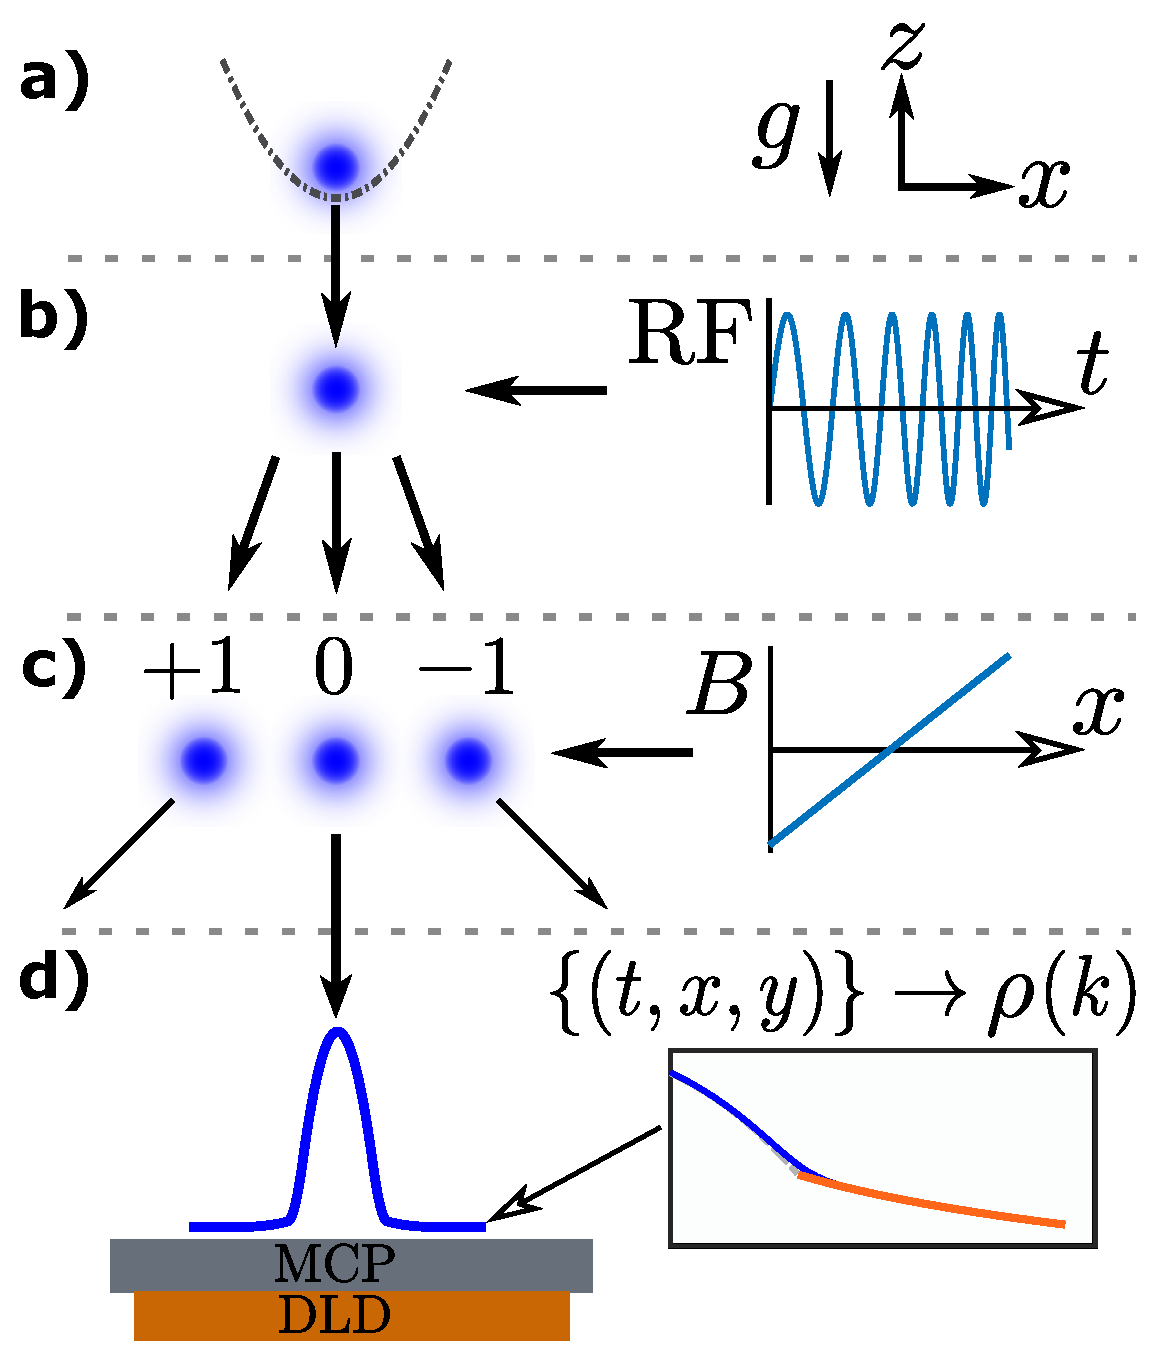
\includegraphics[width=0.4\textwidth]{fig/depletion/main/exp_cartoon}
% % 	    \caption{Sketch of experimental sequence.
% 	A BEC is released from a harmonic trap with (a) and expands during freefall before being split into a superposition of the $m_J\in\{-1,0,1\}$ states (b) by an RF chirp.
% 	A magnetic field gradient separates the clouds (c) ensuring that only the magnetically insentitive $m_J=0$ cloud lands on the detector (d), from which the momentum information is reconstructed.
% 	The quantum depletion lies in the dilute tails at large momentum (inset).}
% % 	    \label{fig:sequence}
% % 	\end{figure}

	


% % \section{Analysis} 

% % 	\begin{figure}[t]
% % 	        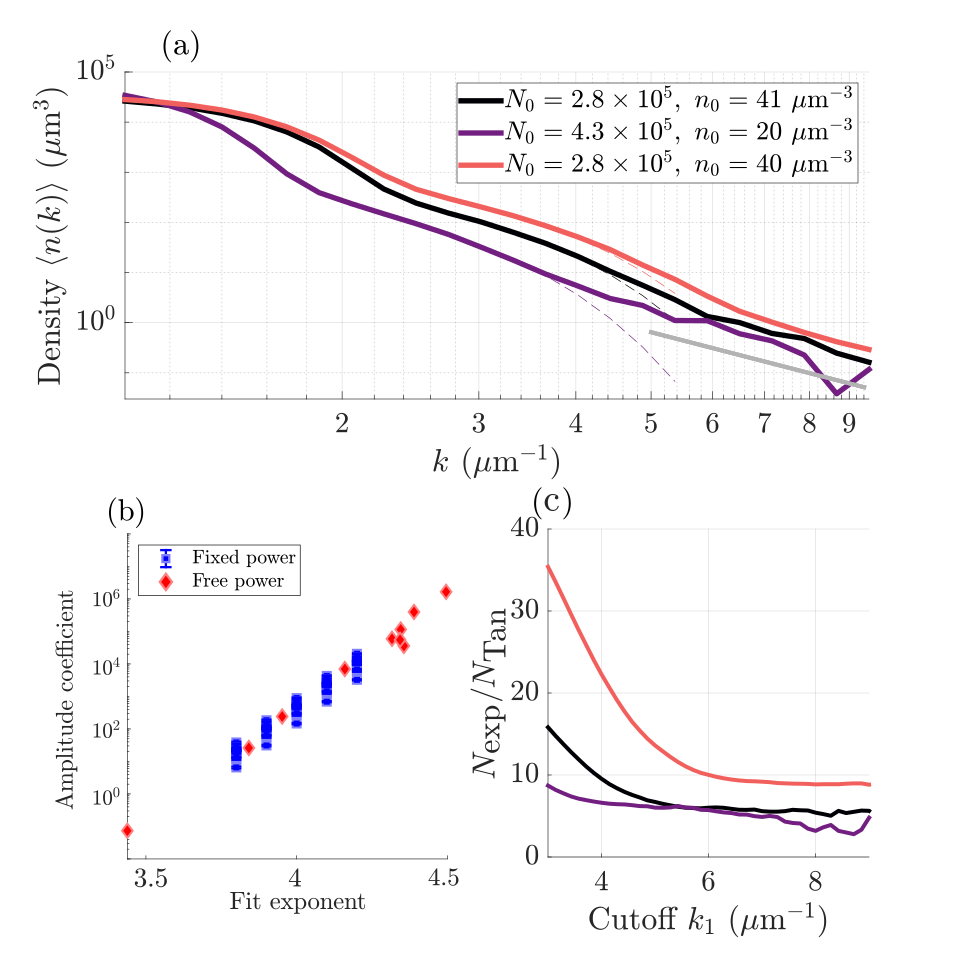
\includegraphics[width=0.5\textwidth]{fig/depletion/main/contact_determination_rev}
% % 	        \caption{The empirical density of particle momenta (a) for different peak densities, where fits to the thermal parts (dashed lines) display exponential decay, which give way to the depletion region, which decays appears to decay with $k^{-4}$ (grey dot-dashed line).
	
% % 	        In (b) we demonstrate the sensitivity of the fitting parameters to constraints in the power law.
% 	Blue squares show the amplitude coefficient $C$ given an exponent $\alpha$ fixed at five values in the range [3.8,4.2], applied to all data sets.
% 	For comparison, leaving $\alpha$ as a fit parameter gives a wide variation in best-fit exponents and scale coefficients.
% % 	        In (c) we show a way around this issue by comparing the number of atoms within the depletion region with the predictions of Eqn.
% 	(\ref{eqn:pred_num}).
% 	We fix $k_2=10\mu\textrm{m}^{-1}$ and $\phi_c=\pi/3$ to define the ROI, and show that $C_\textrm{exp}$ is not significantly dependent on $k_1$ in the depletion region $k\gtrsim6\micron^{-1}$.}
% % 	        \label{fig:cdfplot}
% % 	\end{figure}


% % 	In Fig.
% 	\ref{fig:cdfplot} (a) we show the empirical density $n(k)$ for three representative data collection runs.
% 	The three regimes of the condensate, thermal depletion, and quantum depletion span over five orders of magnitude in density.
% 	The thermal part of the distribution is well fitted by the momentum distribution of an ideal Bose gas,
% % 	\begin{equation}
% % 		n_T(k) = N_T \frac{g_{3/2}\left(\exp(-k^2 \lambda_{dB}^2/4\pi)\right)}{1.202(2\pi/\lambda_{dB})^3}
% % 		\label{eqn:th_fun}
% % 	\end{equation}
% % 	wherein the thermal de Broglie wavelength $\lambda_{dB} = \sqrt{2\pi\hbar^2/(m k_B T)}$  yields an estimate of the temperature $T$ (between 100 and 320 nK (accurate to order 10\%) in our experiments).
% 	Here, $g_{3/2}(\cdot)$ is the standard Bose integral and $N_T$ is the number of atoms in the thermal part.
% % 	The thermal population decays exponentially with $k$, as shown in Fig.
% 	\ref{fig:cdfplot} (a), and hence cannot account for the counts we observe beyond $k\gtrsim 5~\micron^{-1}$.
	
% % \subsection{Issues with analysis of power laws}	

% % 	However, fitting histograms with power-law functions is prone to biased estimates of parameters and drastic underestimation of uncertainties, especially when data is available over less than a couple of decades of dynamic range \cite{Clauset09,Virkar14}.
% 	We first demonstrate some issues with this approach, then discuss our alternative approach.
% % 	If we augment the fit function (Eqn.
% 	(\ref{eqn:th_fun})) with power-law term of the form $C/k^\alpha$, the average exponent of over all runs is 4.2(4).
	
% % 	For comparison, the prior work \cite{Chang16} reported power-law tails with an exponent 4.2(2).
% % 	At first glance, one could simply determine the amplitude of the tails by fixing the exponent to 4, and perhaps achieve better results by using a fit weighting proportional to $k^4$.
	 
% % 	However, as we argue here, there are two issues which preclude such an appealing approach.

% % 	First, in Fig.
% 	\ref{fig:cdfplot} (b) we illustrate how the exponential relationship between the scaling exponent $\alpha$ and the scale coefficient $C$, given the same data.
% % 	% hen fitting a power-law of the form $Ck^{-\alpha}$ to fixed data.
	
% % 	The coefficient $C$ varies over about three orders of magnitude as one uses different exponents $\alpha$ which lie within the range of uncertainties reported here and in the prior work \cite{Chang16}.
	
% % 	For example, fixing $\alpha=4$ in our fits (within the systematic variation) yields a fit amplitude which differs by from the best-fit value by up to a factor of order $100$.
	
% % 	Furthermore, this problem is not captured by the error estimates in the fitting routines: The error bars representing the uncertainty in fit amplitude are smaller than the markers used in Fig.
% 	\ref{fig:cdfplot} (b).
	
% % 	Finally, a linear fit shows that $d \log_{10} C/d\alpha \approx 6.8$, from which we can find the exponent that would yield an amplitude in agreement with Eqn.
% 	(\ref{eqn:pred_scaling}).
	
% % 	This turns out to be approximately 3.9, which is not distinguished with statistical significance from the results of the fitting procedures described here.
	
% % 	Conversely, we can estimate that the best-fit exponents reported in the prior work would lead to scale coefficients a factor of about 23 greater than their conclusions.
	
% % 	This demonstrates that the choice of fit exponent has an outsize influence on the estimate of the corresponding amplitude.
	
% % 	It would be easy to choose $\alpha$ which is not statistically significantly different from the best-fit estimates and arrive at a conclusion which agreed perfectly with the predictions of Eqn.
% 	(\ref{eqn:pred_scaling}), or indeed essentially any tail amplitude one wants.

% % 	Second, a deceptively reassuring result can be found by multiplying the empirical density by $k^4$, observing a flat region, and adding a constant term in an appropriately scaled model of the thermal region (i.e.
% 	Eqn.
% 	(\ref{eqn:th_fun}) multiplied by $k^4$).
	
% % 	In fact, this offers no such recourse.
% % 	Suppose the density decays as some $C k^{-(\alpha+\epsilon)}$: then the scaled density is simply $C k^{-\epsilon}$.
	
% % 	We showed above that a variation of the exponent on the order of a few per cent is both within the systematic error of the fitting procedure and also sufficient to yield drastically different conclusions.
% % 	A variation in $\alpha$ of this size would manifest as a difference of only a factor of order $2^{0.1}\approx1.07$ over the range $5\micron^{-1}\gtrsim k\lesssim10\micron^{-1}$, which is the entire region investigated both here and in the prior work.
% % 	This variation of less than $10\%$ is swamped by the noise in the individual density profiles and is not distinguishable from the run-to-run variation in the power law.

% % 	In sum, there are problems with fitting power laws and it is not clear that the conclusions drawn from such an analysis are insightful even at the best of times.
% % 	In general, determining the exponent of a power law is difficult and requires data over several orders of magnitude in scale \cite{Clauset09,Virkar14}.
% % 	\com{In this case, one could argue that there is a physical rationale for employing $\alpha=4$, but...}
% % 	The preferred statistical tools for analysing power law distributions are maximum likelihood estimators \cite{Goldstein04,Clauset09,Virkar14,Hanel17}, but these are unsuitable here because there are multiple  sources of detection events (discussed further in Appendix A).
	
% % 	Therefore it may not be possible to precisely determine the exponent of a putative power law decay for purposes of the comparison with theory.
	
% % 	We circumvent this issue by using a simpler point of comparison: the number of atoms detected within a region of interest (ROI).
% 	Moreover, we will show that the population of the tails depends on the condensate parameters in agreement with the theory of the contact, albeit up to a constant factor.
	
% % \subsection{Quantifying excess tail amplitude}

% % 	Under the null hypothesis that the \emph{in situ} depletion survives the expansion and escapes the condensate undisturbed, one can integrate Eqn.
% 	(\ref{eqn:pred_scaling}) to predict the expected number of atoms whose wavevector has a modulus in the interval $k\in (k_1, k_2)$, 

% % 	\begin{align}
% % 	\mathcal{N}_\textrm{Tan} &=\frac{\mathcal{C}}{2\pi^2}\left(\frac{1}{k_1}-\frac{1}{k_2}\right)
% % 	\label{eqn:pred_num}
% % 	\end{align}
% % 	 % The noise floor is set by the detector's dark count rate, which contributes an average of less than 1 counts to the region of interest per shot
	
% % 	The null hypothesis can be compared with the experimental results once the bounds of the ROI have been specified (namely, the values $k_1$ and $k_2$, and the solid angle of integration).
% 	We face a tradeoff in the choice of $k_2$ and the minimum elevation angle $\phi_c$ in defining the region of interest.
% 	This is because the field of view of our detector is limited by the 40mm radius of the circular detection surface to $\lesssim5\times 10^6$ m$^{-1}$ in the $(x,y)$ plane, which is only just sufficient to reach past the edge of the thermal region.
% 	The collection volume is maximized for $\phi_c=\pi/3$ rad and $k_2=10^7$ m$^{-1}$, centred on the BEC.
% 	This amounts to an ROI consisting of two vertically oriented conical sections, each with half-angle $\pi/6$, encompassing a total solid angle of $0.13\times 4\pi$ steradians.
	

	
% % 	In Fig.
% 	\ref{fig:cdfplot} (c) we compare the number of detected atoms, corrected for state transfer and detection efficiency, with the predictions obtained from Eqn.
% 	(\ref{eqn:pred_num}) as a function of the lower bound $k_1$ with $k_2=10~\micron^{-1}$ and $\phi_c=\pi/3$.
	
% % 	We consider the average of the quantity $C_\textrm{exp}=N_\textrm{exp}/N_\textrm{Tan}$ over the range $6~\micron<k<10~\micron$, outside the thermal region, as a test statistic for the null hypothesis.
% % 	The uncertainty in a single run is identified as the variance in the estimate over the ROI.
% % 	Averaging over all runs yields an average of 8(1) times as many counts as predicted by Eqn (\ref{eqn:pred_num}), where the final uncertainty is the standard error in the mean and only the most significant digit is shown.
% % 	Thus, while the observed momentum distribution appears consistent with a $k^{-4}$ asymptotic decay, the amplitude of these tails contradicts the null hypothesis of Eqn.
% 	(\ref{eqn:pred_num}) by 5.4$\sigma$.
% 	This would seem to be a count against the interpretation of these tails as a signature of the quantum depletion.
% 	However, we note two pieces of evidence that give weight to this interpretation.
	
% % 	% While at first glance this seems consistent with the fitting procedure, we find that the latter is not stable inasmuch as....	
	
% % \subsection{Consistency in effect size scaling}


% % 	First, the amplitude of the tails scales with $\bar{\omega}$ and $N_0$ in a manner consistent with Eqn.
% 	(\ref{eqn:TotalHarmonicContact}), which can be seen in Fig.
% 	\ref{fig:results_comp}, where we show the estimated contact $C_\textrm{exp}$ obtained by inverting Eqn.
% 	(\ref{eqn:pred_num}).
	
% % 	On one hand, the linear scaling of $C_\textrm{exp}$ with the product $N_0n_0$ is consistent with Eqn.
% 	(\ref{eqn:pred_scaling}).
	
% % 	In fact, this means $C_\textrm{exp}$ scales with $\left(\omega^6 N_0\right)^{1/5}$, i.e.
% 	as predicted by Eqn (\ref{eqn:TotalHarmonicContact}).
	
% % 	Indeed, if we consider the data from each trap configuration separately, the results are also consistent with the same scale factor as above.
% % 	In the absence of another known quantity which exhibits this specific nonlinear scaling relationship, we conclude this line of evidence is supportive of the tails as originating in the quantum depletion.
	
% % 	Second, we find evidence in our simulations (see next section) that the momentum-space signature of the quantum depletion does survive the condensate expansion, and indeed appears in excess of the predicted \emph{in-situ} depletion.
% 	Moreover, several features common to both experimental and simulated momentum distributions emerge, strengthening the identification of the momentum tails with the quantum depletion.
	

% % 		\com{Remarkably, if we do fix $\alpha=4$ then we find fit coefficients that are, on average, 7.8(1.7) times the predicted contact, whereas the fits with free exponents produce a wide range of coefficients, of the order of $4(8)\times10^3$ times the value of the contact calculated using Eqn.
% 	\ref{eqn:pred_scaling}, where the uncertainty is the standard deviation of the fit coefficients.

% % 		In short, it seems that fiddling with the exponent (even by only 0.2 our of 4) is not analytically justified.
% 	This might be ameliorated if there was good physical reason to assume that we are looking at a fourth-power decay, but this is motivated reasoning: In the question of whether or not this is quantum depletion, an almost-matching power law is not a smoking gun, and the sensitivity of the conclusions is remarkable.
% 	More remarkable is the fact that despite these methodological issues, in this specific instance the agreement with a more stable method should not be seen as vindication, but rather as good luck.}


% % 		 Don't seem to have the statistical strength to comment on the istortion of the profile
% % 		Second, we have similar deviation from the power-law distributed momenta in semiclassical simulations.
% 	By simulating the motion of particles with a power-law momentum distribution as they interact with an expanding parabolic mean-field potential in three dimensions, one finds increase in the weight of the momentum tails at small momentum, but the large-$k$ particles are unaffected.
% 	This causes a deviation from the power-law behaviour and a decay slightly faster than $k^{-4}$.
% 	Indeed, a note published by one of the authors of \cite{Chang16} found this effect in 1D \footnote{available via https://web.archive.org/web/20210506045825/https://github.com/rocksonchang/Helium-iPythonNotes/tree/master/20160629\%20-\%20Meanfield\%20kick} and we made similar observations in 3D semiclassical simulations.
% 	Therefore, the exponent slightly greater than 4 is not obviously inconsistent with the population arising from the quantum depletion.
% 	What is surprising is that the amplitude is so much greater than expected, and so we turn to our simulations for further insight.
	
% % 	\begin{figure}[t]
% % 	        \includegraphics[width=0.5\textwidth]{fig/depletion/main/results_comp}
% % 	        \caption{Comparison of simulations and experiments.
% 	The inset is a zoomed view.
% 	 From our empirical data (ED) we determine the empirical contact $C_\textrm{exp}$ which is linear in the product $N_0n_0$ (as predicted by Eqn.
% 	(\ref{eqn:pred_scaling})), but 8(1) times more sensitive (Av) than the prediction by the Tan theory (TT).
% 	The simulated contact of BECs in a cigar-shaped trap (CT) are consistent with (TT) before release and increases after expansion (CE), but by less than the experiment.
% 	A slow relaxation of the tight axes of the cigar trap (CS) leads to a reduction in the simulated contact.
% 	Simulations of a spherical trap (ST) show a negligible increase after expansion (SE).
% 	The prior \mhe result \cite{Chang16} (IO) is shown for comparison (dashed line)}
% % 	        \label{fig:results_comp}
% % 	\end{figure}

% % \subsection{Experimental details}

% % \subsubsection{Trap configuration and calibration}

% % 	We prepared our BECs with via forced evaporative cooling in a harmonic magnetic trap with trap frequencies $(45,425,425)$ Hz and a DC bias stabilized by our auxiliary field compensation coils \cite{Dall07,Dedman07}.
% 	For the tight trap we increased the coil current after the cooling sequence to obtain trapping frequencies $(71,902,895)$ Hz, ramping the field as a sigmoid step function to minimize in-trap oscillations.
% 	Note that the weak ($x$) axis of the trap is horizontal, with tight vertical confinement.
% 	The trap remained on for 150ms before switching the trap off with a $1/e$ time of $\approx38\mu$s.
% 	The condensates were allowed to expand for 2ms before we transferred some of the condensate into the magnetically insensitive $m_J=0$ state via Landau-Zener sweep to prevent distortion by stray magnetic fields.
% 	The RF pulse was created by a  function generator, amplified, and applied to the experiment chamber by a coiled antenna inserted into the BiQUIC coil housing.
% 	The pulse swept from 1.6-2.6MHz over 1ms and was centred on the fine structure resonance between the $m_J$ states.
% 	The transfer efficiencies $\eta_j$ for each of the $m_J = j$ states is discussed in the next section.
% 	The sweep was $10^6$-fold wider than the Doppler broadening of the BEC which ensured uniform transfer at all momenta.
% 	Immediately after the RF sweep, the bias coils are switched off and auxiliary push coils in the vertical (Z) and weak horizontal (X) axes are activated using a fast MOSFET switch to implement a Stern-Gerlach separation of the $m_J = -1,~0,$ and $+1$ pulses.

% % 	We use a Roentdek DLD80 multichannel plate and delay-line detector stack \cite{Manning10} located 859mm below the trap, which registers the arrival times and positions $(t_i,x_i,y_i)$ of each atom, indexed by $i$.
	
% % 	The velocity of each atom relative to the centre of mass of the cloud is calculated by $(v_x,v_y,v_z) = t_{i}^{-1}(x_i-\bar{x},y_i-\bar{y},g_0(\tau^2-t_{i}^{2}))$, where $g_0$ is the local gravitational acceleration and the overbar denotes the within-shot average and $\tau=417$ ms is the time of flight of the centre of mass.
	
% % 	The far-field momentum is thus obtained via $m\textbf{v} = \hbar\kvec$.
% % 	The velocity conversion assumes a point source but carries a negligible error of a few ppm as the in-trap BEC size is smaller than the detector resolution.
	
% % 	The space and time resolution of the detector are 100 $\mu$m and 3 $\mu$s, respectively \cite{Henson18}, and the detector efficiency of $8(2)\%$ was determined from the collection efficiency of correlated atoms on the opposite sides of scattering halos \cite{shin19,shin20,Jaskula10}.
	

% % \subsubsection{Determining transfer efficiency}

% % 	To calibrate the transfer efficiencies, we applied a weaker Stern-Gerlach than for the depletion measurement, resolving each $m_J$ cloud on the detector, as illustrated in Fig.
% 	\ref{fig:frac_cal}.
	

% % \begin{figure*}[!t]
% % 	\begin{center}
% % 		\includegraphics[width=\textwidth]{fig/depletion/main/frac_cal_profile}
% % 		\caption{Determining the RF transfer efficiency.
% 	The time-of-flight profiles of each pulse are resolved (a) by applying a weak Stern-Gerlach pulse during the time of flight.
% 	The pulses are aligned with respect their centre-of-mass (b) and used to determine the pointwise fraction ((c), dotted line).
% 	Detector saturation is evident in the peaks (dashed lines), but not in the thermal tails (solid lines), which are used to compute the transfer efficiency.
% 	Because of its lower flux, the $m_J=-1$ pulse does not show evidence of saturation (d) and is used to determine the thermal fraction.}
% % 		\label{fig:frac_cal}
% % 	\end{center}
% % 	\end{figure*}

% % 	The efficiencies $\eta_J$ cannot be calculated by counting the atoms in each cloud because the detector saturates during the peak condensate flux, but we can compare the thermal parts.
% 	We align each cloud along the time (Z) axis and compute the pointwise fraction of the atomic flux $\phi(t)$ accounted for by each cloud, $\eta_j(t) = \phi_j(t)/\sum_j\phi_j(t)$, as depicted in Fig.
% 	\ref{fig:frac_cal}.
% 	The ratio of densities between the clouds is roughly constant in the thermal part, indicating the absence of important saturation effects and a spin transfer that is independent of $k$.
% 	The fraction of the original cloud transferred into each $m_J$ state is determined by taking the average $\langle\eta_j(t)\rangle$ over the thermal tails.
% 	We find these efficiencies are approximately 74\%, 24\%, and 2\% in all runs for the $m_J=+1$, 0, and -1 states, respectively.
	
% % 	While the $m_J=0$ and $m_J=1$ clouds clearly saturate the detector, the small fraction ($\approx2\%$) of the atoms transferred to the $m_J=-1$ state does not (Fig.
% 	\ref{fig:frac_cal} (d)).
% 	A bimodal fit to the condensed and thermal parts, plus constant background, yields an estimate of the thermal and condensed fractions.
	


% % % \subsection{Determination of thermal fraction}
	

% % % 	\begin{figure}[!h]
% % % 	\begin{center}
% % % 		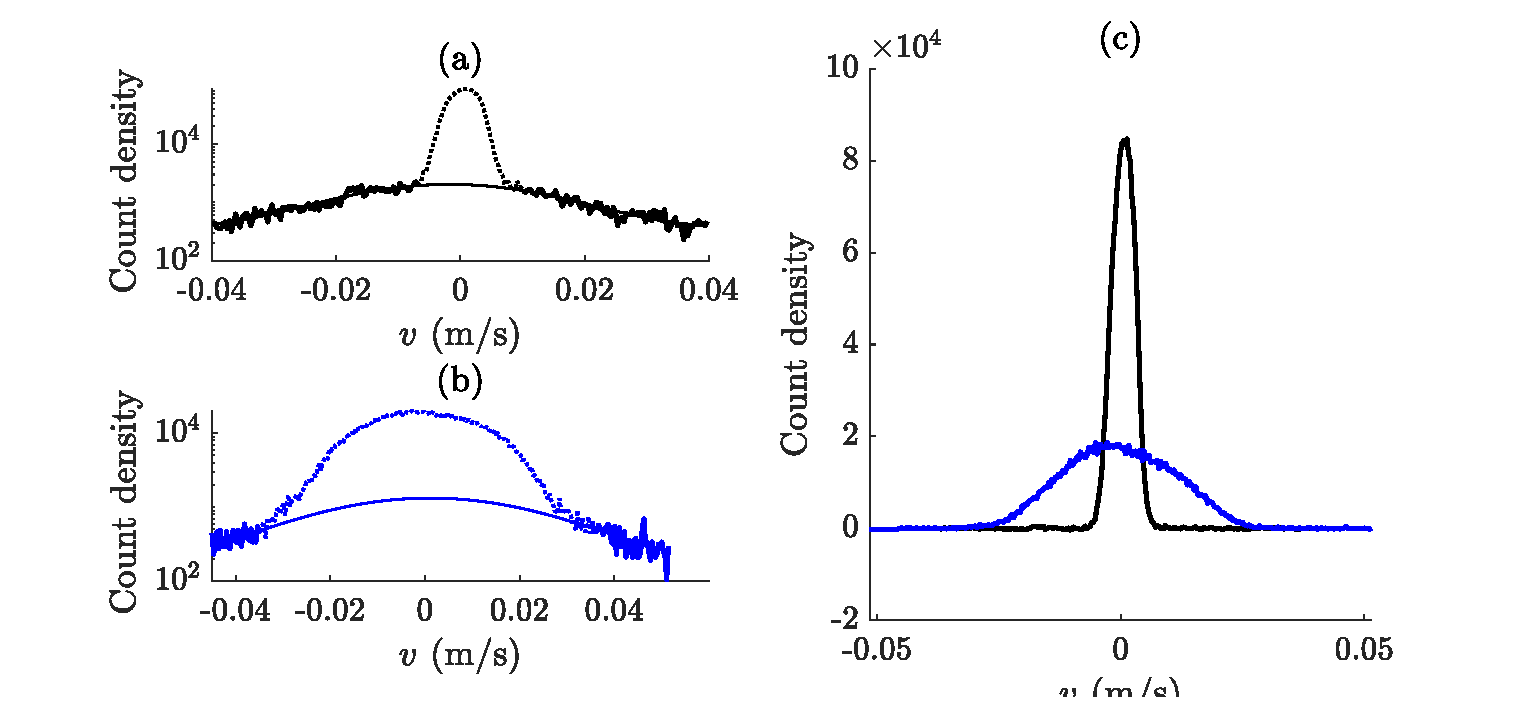
\includegraphics[width=0.8\textwidth]{fig/depletion/main/m1_frac_anal}
% % % 		\caption{Comparison of thermal fits in the unsaturated $m_J=-1$ pulse including 138 shots.
% 	The weak (X) and strong horizontal (Y) trapping axes are shown in (a) and (b), respectively.
% 	\org{would be helpful to label $v_x$ and $v_y$ to make it self-evident at 1st glance.} Both projections display a bimodal peak, with the condensate (dotted lines) and thermal parts (thick solid lines) easily distinguished.
% 	Fitting a Gaussian profile (thin solid line) to the velocity distribution of the thermal part yields the thermal number and temperature.
% 	Subtracting the fit leaves the condensate profile (c) which can be \blu{\dots something\dots} yields the condensed number.}
% % % 		\label{fig:thermal_frac}
% % % 	\end{center}
% % % 	\end{figure}



% % \subsubsection{Analysis of spin transfer measurements}

% % 	In early tests of our measurement sequence we noticed a contamination of the signal by spurious counts.
% 	We inferred these were remnant counts from the $m_J=+1$ cloud as they were still visible when we ran an experimental sequence without the Landau-Zener transfer.
% 	This contamination appeared in a particular region of our detection image, illustrated in Fig.
% 	\ref{fig:spinpop}.
% 	As such we were able to correct for it by subtracting their contribution from the counts collected during measurement shots.
% 	Generally, fewer atoms can be attributed to this noise ($\leq~1$ atom per shot, on average) than would be required to explain the discrepancy described in the main text ($5-10$ counts per shot).
% 	While the cause of the cross-contamination is unclear, we observe that the count density outside the region of interest is similar in both the shots with the RF pulse and those without.
% 	We hypothesize that the remnant counts are atoms transferred into the $m_J=0$ state by non-ideal behaviour of the Stern-Gerlach pulses.
% 	We note that only about one in a million atoms from the $m_J=1$ cloud present in this manner in a given shot.

% % 	As mentioned in the main text, the presence of these counts also prevents a straightforward application of a maximum-likelihood estimator (MLE) to determine parameters of the power-law region.
% 	The basic principle of the MLE is to assume a functional form for the probability distribution $p(x|\theta)$ underlying the observed data $x$, and dependent on some parameters $\theta$; the zero of the derivative of the \emph{likelihood} function $L(\theta|x)$ with respect to the parameters $\theta$ then yields the most-probable parameter values given a set of observations $x$.
% 	In our context, one can assume a functional form for the probability distribution underlying atomic detection events (via a wavefunction ansatz).
% 	The detector dark count rates can also be incorporated by assuming a uniform distribution, although this necessitates a cumbersome procedure to retain proper normalization.
% 	Such an analytical treatment does not readily permit the inclusion of an empirical density estimate which itself includes the aforementioned dark count rate.
% 	Instead, we opt for the simpler approach described in the main text.

% %     \begin{figure}[!b]
% % 	\begin{center}
% % 		\includegraphics[width=\columnwidth]{fig/depletion/main/spinpop}
% % 		\caption{Measured contribution of the detector dark counts and spurious spin counts to the time-of-flight profile.
% 	We accounted for the pulse at around 550ms and subtracted it from the measured profiles when computing the contact.
% 	After removing this background term, the density profiles above and below the condensate agree, indicating convergence on the true signal.
% 	For reference, the peak flux of the $m_J=0$ condensate is about a thousandfold greater than the peak shown here.}
% % 		\label{fig:spinpop}
% % 	\end{center}
% % 	\end{figure}

% % 	% \begin{figure}[!h]
% % 	% \begin{center}
% % 	% 	\includegraphics[width=\textwidth]{fig/depletion/main/profile_overlay}
% % 	% 	\caption{Comparison of average time-of-flight profiles over a single data run for the quantum depletion measurement shots (blue, 871 shots), transfer efficiency calibration (black, 112 shots), detector dark counts (red, 871 shots), and spurious counts (dot-dash, 895 shots).
% 	The time window bounded by $|k|\leq 10\mu$m is indicated with dotted lines.
% 	Shaded area is the standard error over the entire run.}
% % 	% 	\label{fig:tof_profile}
% % 	% \end{center}
% % 	% \end{figure}




% % % Note that the temps disagree between axes, but within axes between clouds they are consistent(....ish).
% 	This means we can use the profile ratio method, which is also consistent with comparing the thermal number from the fits.
% % % Perhaps comment on the thermal-subtracted part; the TF profile should have a sharp cutoff, but the smooth edges are suggestive evidence of this roll-off

% % % \begin{figure}
% % % 	\centering
% % % 	\includegraphics[width=0.5\textwidth]{fig/depletion/main/counts_per_run}
% % % 	\caption{Number of counts detected in the region of interest in the depletion measurement (a), the spin mixing calibration (b), and the dark count calibration (c).
% 	An average of 3.0(5) counts were detected in the ROI in the spin-mixing calibration shot, and the background count rate was 0.4(2) counts per shot.
% 	Separate lines indicate separate \emph{runs}, i.e.
% 	sequences of shots with fixed parameters.}
% % % 	\label{fig:num_counts}
% % % \end{figure}


% % \subsection{Peak density calibration}

% %     The quantum depletion and contact are both predicted to depend solely on the condensed number and trapping frequencies via the condensate density, hence it is important to determine both quantities accurately.
% 	In the Thomas-Fermi approximation, the peak density of the condensate can be written as $n_0 = \mu/g$, where $\mu$ is the chemical potential, $g=4\pi\hbar^2a_{1,1}/m$ is the effective interaction strength, $m\approx6.6\times10^{-27}$ kg is the atomic mass, and $a=7.512$ nm is the s-wave scattering length between pairs of atoms in the $m_J=1$ state \cite{Moal06}.
% 	The sole experimental parameters in the expression for the peak density (Eqn.
% 	\ref{eqn:n0}) are $\bar{\omega} = \left(\omega_x\cdot\omega_y\cdot\omega_z\right)^{1/3}$,  the geometric trap frequency, and $N_0$, the number of atoms in the condensate.
% 	During these calibration runs we simultaneously determine the total atom number $N$ and trap frequency $\bar{\omega}$ in a single shot using a pulsed atom laser and use the thermal fraction (as below) to determine the condensed number $N_0$.
	

% % 	The pulsed atom laser consists of a series of Fourier-broadened RF pulses centred on the minimum Zeeman splitting in the trap.
% 	The pulse transfers atoms in the trap to the untrapped $m_J=0$ state with an approximately constant transfer rate across the cloud.
% 	We outcouple approximately 2\% of the atoms per 100$\mu$s pulse for $\approx$200 pulses, which eventually depletes the entire trap.
% 	The atom laser thus prevents the detector from saturating and allows an accurate determination of the atom number, up to a factor of the quantum efficiency.
% 	We determine the trapping frequencies by inducing centre-of-mass oscillations with a magnetic impulse, and finding the oscillation period from the atom laser pulses \cite{henson18ML}.



% % \section{Numerical simulations}
% % \label{STAB}

% % 	We performed simulations of the BEC expansion from harmonic traps using the first principles STAB method \cite{Deuar11,Kheruntsyan12}.
% 	The simulations included a cigar-shaped trap (marked CT in Fig.
% 	\ref{fig:results_comp}) with parameters matched to the experimental conditions.
% 	The in-trap state was consistent with the adiabatic sweep theorem before release from the trap.
% 	Following expansion from the cigar trap (CE in Fig.
% 	\ref{fig:results_comp})), the simulated tail amplitude increased and stabilized within a few hundred microseconds, much sooner than the 2ms delay between the trap release and application of the rf and Stern-Gerlach pulses.
% 	Fig.
% 	\ref{fig:time_dep_theory} shows time evolution of the tail amplitude for the simulated traps using the same ROI as the experimental setup.
% 	 In this configuration the steady-state value of the momentum tails was a factor of 1.64(9) above the predictions of Eqn.
% 	(\ref{eqn:pred_scaling}).
	

% % 	To understand the disagreement with earlier theory \cite{Qu16}, which predicted no depletion survival, we also investigated the effect of adiabatic expansion on the in-trap depletion by simulating a slow decrease of the transverse trapping frequencies by a factor of two (CS), and found that the in-trap contact decreased roughly as predicted by Eqn.
% 	(\ref{eqn:pred_scaling}) in these instances --- see the dashed line in Fig.~\ref{fig:time_dep_theory}.
	

% % 	We also found that the factor of disagreement (i.e.
% 	$C_\textrm{sim}/C_\textrm{Tan}$) between Eqn.
% 	(\ref{eqn:pred_num}) and the simulated tails depends on the angle choice of cutoff angle $\phi_c$.
% 	Put another way, the momentum distribution in the simulations is anisotropic and takes the form $f(\theta,\phi)/k^4$.
% 	We note that the average of an angle-dependent power law decay over a region $\Omega$ is simply $\langle f(\theta,\phi)\rangle_\Omega/k^4$, preserving the power-law behaviour.
% 	We find a similar effect in the experimental data as well, albeit with low statistical significance owing to the small signal-to-noise.
% % 	Specifically, we find that $C_\textrm{exp}$ is larger for smaller collection regions that are more tightly concentrated about the vertical (strong) trapping axis, whereas larger collection angles (including areas closer to the weak axis) produce a lower $C_\textrm{exp}$.
% % 	We quantify this effect in Tab.
% 	\ref{tab:angle_dep} and propose physical origins of our observations in the next section.
	

% % 	\begin{figure}[t]
% % 	        \includegraphics[width=0.5\textwidth]{fig/depletion/main/time_dep_theory}
% % 	        \caption{Simulations of condensates released from a cigar-shaped trap show an increase in contact after the trap release, stabilizing after a time on the order of $1/\omega_x$, several hundred $\mu$s.
% 	The relative difference between in-trap and expanded contact increases with the density of the condensate.
% 	For comparison, the experimental control pulses are implemented after 2ms of expansion.
% 	In contrast, when the transverse trapping frequencies are reduced by half (dotted line), the in-situ contact relaxes.}
% % 	        \label{fig:time_dep_theory}
% % 	\end{figure}

% % 	\begin{table}[b]
% % 		\begin{tabular}{c c c}
% % 			\hline\hline
% % 			Half-angle &	$C_\textrm{exp}/C_\textrm{Tan}$ &	$C_\textrm{sim}/C_\textrm{Tan}$\\
% % 			\hline
% % 			10	&	9.3(3.3) &	2.2(3)\\
% % 			20 	&	8.7(1.8) &	1.9(2)\\
% % 			30	&	8.0(1.3) &	1.6(1)\\
% % 			\hline\hline
% % 		\end{tabular}
% % 		\caption{The excess of detection events over the expected number depends on the choice of angular bounds for the ROI.
% 	We show the average factor of disagreement between experimental and predicted counts for three half-angles defining the two vertically oriented conical sections.
% 	For comparison, we show the factor of disagreement for the $C_\textrm{sim}/C_\textrm{Tan}$simulated case where $n_0=44~\micron^{-3}$.}
% % 		\label{tab:angle_dep}
% % 	\end{table}

% % % \include{sim_part}


% % \section{Discussion}

% % 	We interpret these results as an indication that the depleted atoms are accelerated by the non-uniform mean-field energy of the condensate during the expansion.
% % 	In detail, after a quench into the free particle regime, the condensate expands hydrodynamically on timescales of $1/\omega$.
	
% % 	This is an adiabatic process for the low momentum depletion, whereby some depleted atoms are absorbed back into the condensate in agreement with \cite{Qu16}.
% % 	However, the characteristic time for reabsorption is $\hbar/gn_0$, slow enough that quasiparticles in the particle branch of the Bogoliubov dispersion have sufficient velocity to escape the expanding cloud without being reabsorbed and thus transition to free atoms.
	
% % 	This effect contributes to the disagreement between \emph{in situ} and measured tail amplitudes, hence $C_\textrm{exp}$.

% % 	Moreover, an atom inside the BEC experiences an effective force from the gradient of the mean-field potential $\textbf{F} = -4\pi\hbar^2a \nabla  n(x)/m$.
	
% % 	This endows escaping depleted particles with a greater momentum, increasing the weight of the tails in the far-field.
	
% % 	This effect is exacerbate in light atoms like $^{4}$He: because the acceleration scales with $1/m^2$, it would be suppressed by a $\sim500$-fold in $^{87}$Rb experiments \cite{Makotyn14}.
	
% % 	Further, it is much easier for depletion atoms to escape and be accelerated in the transverse x-y directions from an elongated cloud because the distances $R_{TF}=\frac{1}{\omega}\sqrt{2gn_0/m}$ are reduced by $\bar{\omega}/\omega_{x,y}$, whereas the initial mean depletion velocities \textit{in situ} $v\sim \sqrt{2gn_0/m}$ are isotropic.
% % 	Indeed, spherical clouds (SE) exhibit a much weaker effect than the elongated clouds (CE) owing to the longer escape time.
% % 	Furthermore, we find some evidence that this anisotropic feature is present in our experimental data.
	
% % 	The hypothesis that this conjunction underlies the observed effects is further supported by our simulations: We observe a decrease in the total number of depleted particles (reabsorption) and a simultaneous increase of the large-k population (forcing).
	
% % 	This constitutes a partial explanation of the experimenal findings too, exhibiting important similar features including the anisotropic distribution and nonlinear scaling consistent with the quantum depletion.
	

% % 	\com{Two factors to address: Detector efficiency and the Landau-Zener transfer}


% % 	However, a mystery remains: Why is the excess depletion some four times greater than accounted for by this picture? This issue should be resolved in order to interpret far-field observations in terms of the in-trap physics of interest.
	
% % 	This question invites complementary studies of the \emph{in situ} depletion in \mhe BECs.
	
% % 	The cause of the contact anomaly could be elucidated by determining whether it originates in the trapped condensate, or is generated during the trap release and expansion.
	
% % 	Such an investigation requires an \emph{in situ} probe of the contact, such as RF spectroscopy or Bragg spectroscopy.
% % 	The latter may be the most fruitful of the two simply because of the difficulty of interpreting the results from the former, which we sketch here.
	
	
% % 	The basic principle of RF contact spectroscopy is to apply a monochromatic RF probe which is detuned from the resonance between two spin states, coupling atoms in the initial spin state to an untrapped channel.
	
% % 	One then performs a differential measurement of the atom number and expects the signal strength to scale as $\omega_\textrm{RF}^{3/2}$ with the detuning from the RF resonance.
% % 	The loss rate is also proportional to the difference of reciprocal scattering lengths $\Gamma\propto(1/a_\textrm{i,i}-1/a_\textrm{i,f})$ between pairs of atoms in initial-initial ($a_{i,i}$) and initial-final ($a_{i,f}$) spin states \cite{Braaten10,Wild12}.
	
% % 	For He$^*$ (spin 1) the scattering lengths $a_{1,1}$ and $a_{1,0}$ are identical \cite{Leo01}, rendering the preferred $m_J=1-m_J=0$ transition unusable.
	
% % 	On the other hand, $a_{1,-1} = 3/7 a_{1,1}$ \cite{Vassen16}, and the singlet transition can be driven without populating the $m_J=0$ state.
	
% % 	In principle this could produce a detectable flux of atoms to perform sensitive in-trap contact measurements, however, collisions in the $^1\Sigma_{g}^{+}$ channel have large Penning ionization rates which lead to significant trap losses \cite{Leo01}.
	
% % 	The ionization products would be detectable by in-vacuum channel electron multipliers but require theoretical work to disentangle from the spectroscopic signal.
	
% % 	Further, while other atomic species offer Feshbach resonances by which to tune the inter-species scattering length (and hence signal or ionization rate), \mhe has no such feature.
	
% % 	While such a measurement is not \emph{prima facie} impossible, Bragg spectroscopy may yield more readily comprehensible results.

	
% % 	\section{Conclusion} 

% % 	Our work expands the growing suite of far-field investigations of quantum depletion \cite{Cayla20,Chang16} and confirms that quantum depletion can, remarkably, survive past the lifetime of its original condensate.
% 	Our findings clarify that how the depletion can be visible in the far-field momentum distribution here and in earlier experiments, and that the hydrodynamic approximation does not capture sufficient short-wavelength information to make detailed predictions about the high-momentum behaviour.
% 	We thus find a partial explanation for the deviation of the far-field distribution from both the predicted in-situ depletion and the hydrodynamic reabsorption: The interplay between coherent absorption of Bogoliubov excitations and the dispersal of the chemical potential into kinetic energy, to which helium is particularly sensitive, result in a growth of the $k^{-4}$ tails of the momentum distribution during freefall.
% 	It would be informative to determine whether this discrepancy originates in the trapped condensate or is due to some unknown non-equilibrium effect during expansion.


% % 	\section{Acknowledgements} We Would like to thank David Clement, Raphael Lopes, Jean Dalibard, and Karen Kherunstyan for their helpful discussions.
% 	This work was supported by Australian Research Council (ARC) Discovery Project Grants No.
% 	DP160102337 and No.
% 	DP190103021.
% 	S.
% 	S.
% 	H was supported by DECRA DE150100315,  J.A.R., D.
% 	K.
% 	S.
% 	by the Australian Postgraduate Award (APA), and K.F.T.
% 	by the Australian Government Research Training Program (RTP) Scholarship.
% 	The simulations by P.
% 	D.
% 	were supported by National Science Centre (Poland) grants No.
% 	2018/31/B/ST2/01871 and 2012/07/E/ST2/01389.

% % \nocite{Manning10,Henson18,shin19,shin20,Jaskula10,Dall07,Dedman07,Moal06,henson18ML,PethickSmith,braaten10,wild12,Leo01,vassen16,Deuar11,Kheruntsyan12,Drummond80,Deuar07,Sinatra00,Kheruntsyan12,Deuar11,Krachmalnicoff10,Lewis-Swan14,Lewis-Swan15,Deuar13,Deuar14,nstab-longpaper,Drummond80,Deuar11,tcorr,Deuar13,FINESS-Book-Ruostekoski,FINESS-Book-Sinatra,Martin10a,Martin10b,Sinatra02,Norrie06,Deuar11,DeuarPhD,Drummond20,stob,nstab-longpaper}

% % \bibliography{bibliography}
% % \appendix
% % %\section*{Supplementary Materials}

%\comment{sections just dumped from main text for now - clean up later}



%Our bespoke software interfaces with the LabView control environment and loops over a sequence of experiments, consisting in this case of: Atom number calibration, Trap frequency calibration, and RF transfer efficiency, followed by 10 data collection runs.

%To calibrate the atom number, we used an RF pulse sequence to create a pulsed atom laser with intensity well below the saturation threshold of our delay-line detector. We corrected the number of detected atoms to account for the quantum efficiency ($\sim$8\%) of our detector. 
%\comment{Should use QD measurements to compute condensate/thermal fraction relative sizes and further improve $N_0$ measurement}.
%\comment{how does this compare to our trap binning? What is the uncertainty of the QE?}

%Together with the atom number, a measurement of the centre-of-mass motional frequencies allowed us to compute the peak density of the condensate. We measured the trap frequency by transient magnetic field to the trapped condensate for $\sim 150\mu s$, forcing centre-of-mass motion in the lab frame. We used the same pulsed outcoupling scheme as in the number measurement, and measured the  centre-of-mass momentum of the cloud at the time of each pulse. Our outcoupling frequency is well below the natural frequency of the confining potential so we used a subsampled reconstruction method to recover the trap frequency. Prior to running experiments we varied the outcoupling pulse frequency to determine in which Nyquist zone the actual trap frequency lies relative to our sampling frequency. We can then obtain the trap frequency to within precision X in a single shot of the experiment by taking a Fourier transform of the centre of mass motion.

%Our calibration sequence provided accurate number and peak density measurements along with the condensate profile. We verified the spherical symmetry of the thermal and depleted fractions, and so compute the momentum density by an average over a large section of the momentum distribution. 

%We verified the fitting method by analysing a test data set of known parameters, which was generated by the Metropolis-Hastings algorithm, and find the method recovers the test set parameters within a factor less than our experimental uncertainties.  


%There may still be errors in the analysis. The fitting procedure apparently produces a good fit, but it may be possible to get indistinguishable or better fits by fixing the exponent of the power law to be some $\alpha\neq 4$. This would challenge the assertion that the cause of the observed profile is in fact quantum depletion.  Assuming the observed data does follow a power law, statistical fluctuations in the high-momentum region become amplified by the $k^4$ scaling procedure and could introduce further error in the estimated Tan constant. \comment{Y-error bars are computed in a fairly ad-hoc way, so ours and Chang may be drastically under-reported...)}Reliably estimating the parameters of a power-law distribution is nontrivial\cite{Clauset2009}, and the robustness of the fitting method above has not been exhaustively tested. The LDA prediction is essentially that the single-particle wavefunctions, hence the single-particle probability distribution over momentum, are affected by many-body effects. One computes the single-particle probability density by dividing the condensate density by the number of particles (hence the $N_0$ term in the LDA), and then the problem of extracting the contact parameter from the data is an exercise in statistical parameter estimation. As shown by Clauset et al \cite{Clauset2009}, fitting these functions tends to produce incorrect estimates of parameters. The method outlined in Clauset was proven to asymptotically converge with probability 1 to the correct fit parameters of a power law distribution, but would need to be extended to derive a maximum likelihood estimator for a power law overlaid on a constant background.


% % \end{document}


% % \begin{abstract}

% % Measurements of Tan's contact in expanding condensate conflict with predictions of the \emph{in situ} quantum depletion.
% 	It is unclear how the depletion survives without a condensate, and even appears stronger in the far-field than before the trap release.
% 	We confirm experimental observations of a power-law decay in the far-field, consistent with the survival of the quantum depletion.
% 	Simulations of our experiment support this conclusion and provide a partial explanation.
% 	A gap between the numerical and empirical results is an open question obstructing studies of quantum depletion in the far field.
% % % max 600chars for PRL
% % % \end{abstract}

% % % \maketitle

% % % \section{Introduction} 
% % A profusion of work on quantum degenerate matter is motivated by the promise of the prototypical coherent phenomenon, superfluidity.
% 	The underlying mechanism of superfluid formation is the Bose-Einstein condensation of collective excitations, which was realized by Bogoliubov \cite{Bogolubov47}.
% 	This finding is of broader importance because the BEC and BCS regimes of supercondictivty are characterized by condensation of molecular dimers and of Cooper pairs, respectively.
	

% % Bogoliubov formulated the problem of a homogeneous system of interacting bosons in terms of a free Bose gas of collective excitations, constituted by pairs of particles with opposite momenta \cite{vogels02}.
% 	The thermal population of quasiparticle modes produces the normal component of a superfluid, while the zero-point population, called the \emph{quantum depletion}, accounts for the large-momentum part of the wavefunction.
% 	The Bogoliubov spectrum exhibits a crossover from wavelike phonon modes to single-particle excitations at momenta larger than the speed of sound in the condensate \cite{steinhauer03}, but this description breaks down in strongly interacting systems \cite{lopes17_quasiparticle} whereas the Tan relations remain valid in the strongly-correlated regime.

% % In a modern addition to the theories of quantum matter, Tan explained how s-wave contact interactions modify the short-range pair correlation function and manifests as a power-law decay in the momentum density \cite{tan08_energetics,tan08_momentum,tan08_virial}.
% 	The contact underpins several universal relations between many-body features and microscopic information in aribitrary spin mixures at any density, temperature, and geometry \cite{combescot09,braaten08,braaten11,werner12_boson,werner12_fermion}.
% 	Emerging evidence for analogous relations in p-wave scattering \cite{luciuk16} and three-body interactions \cite{fletcher17} hints at the prospect of new systematic ways to design thermodynamic features by tailoring the interactions between particles.
	

% % Two defining properties of Tan's contact, known as the adiabatic sweep theorem \cite{tan08_momentum} and generalized virial theorem \cite{tan08_virial}, have been decisively verified via radio spectroscopy \cite{baym07,punk07,braaten10} of degenerate Bose \cite{wild12} and Fermi gases \cite{stewart10,sagi12}.
% 	Bragg spectroscopy has revealed the universality of scaling relations for the pair correlation function \cite{kuhnle10} and the behaviour of the contact across the superfluid phase transition \cite{kuhnle11,mukherjee19,carcy19}, yielding benchmarks for descriptions of strongly-correlated gases \cite{rakhimov20}.

% % The Bogoliubov theory has also yielded accurate predictions of the quasiparticle spectrum \cite{lopes17_quasiparticle,vogels02} and of the depleted population in ultracold atomic Bose-Einstein condensates \cite{xu06,lopes17_depletion} and exciton-polariton condensates in solid substrates \cite{pieczarka20}.
% 	The Bogoliubov spectrum exhibits a crossover from wavelike phonon modes to single-particle excitations at momenta larger than the speed of sound in the condensate \cite{steinhauer03}, but this description breaks down in strongly interacting systems \cite{lopes17_quasiparticle}.
% 	However, detailed study of the quantum-depleted tails of the momentum distribution has been challenging to date because the tails are beneath the noise floor of optical imaging techniques.
% 	A previous experiment sought to use a Feshbach resonance to produce a visible depleted fraction \cite{makotyn14}, but found that the momentum distribution saturated during expansion and did not display a power-law tail.
% 	This was because many-body effects shielded condensed atoms from excitation into the normal component \cite{kira15_hyperbolic,kira15_coherent}.


% % In contrast, another experiment found unexpectedly large momentum tails in the far-field of a Helium BEC released from a harmonic optical trap \cite{chang16}.
% 	This is particularly surprising because conventional wisdom argues that the density decreases adiabatically during expansion \cite{xu06}, justifying treatment with a hydrodynamic approximation wherein the tails are predicted to vanish \cite{qu16}.
% 	Instead, the study \cite{chang16} found momentum tails far stronger even than expected in the cloud before release.
% 	This contradiction implies that either helium condensates violate the minimal assumptions of Tan's theory of the contact \cite{tan08_energetics,tan08_momentum,tan08_virial}, or that far-field momentum measurements are not a straightforward means of examining the quantum depletion even in weakly interacting gases.
% 	It is important to verify and overcome this obstacle, as such measurement could play a central role in studying the microscopic physics of superfluids with ultracold gases.

% % To this end, we revisit the measurement of the momentum distribution of a helium condensate expanding from a harmonic trap.
% 	We conducted experiments using an independent apparatus and analysis, covering a range of densities twice as large as in the prior work \cite{chang16}.
% 	We observe power-law tails in the far field whose amplitude significantly exceeds the predictions of the \emph{in situ} depletion, corroborating the prior work.
% 	Our measurements are complemented by simulations of the time-dependence of the momentum distribution using a stochastic Time-Adaptive Bogoliubov (STAB) method in the positive-P framework \cite{Deuar11,Kheruntsyan12,SOM}.
% 	These show that the non-adiabatic release of the trap is responsible for survival of the depletion, and that the depleted particles acquire additional kinetic energy from the mean-field energy of the condensate during the subsequent adiabatic expansion.
% 	These factors result in an amplification of the momentum tails relative to the \emph{in situ} values and are not captured in the hydrodynamic approximation.
% 	However, quantitative disagreement between our simulations and experimental data rule out the release energy as a complete explanation for the observed excess counts.
% 	We conclude by suggesting an informative complementary approach.
	

% % \section{Experiment} Our experimental sequence, depicted schematically in Fig.
% 	\ref{fig:sequence}, began with BECs with between $2\times 10^5$ and $5\times 10^5$ $^4$He atoms polarized in the $\metastable(m_J=1)$ state and cooled to $\sim$ 300 nK by forced evaporative cooling in a harmonic magnetic trap generated by field coils in a Bi-planar Quadrupole Ioffe configuration \cite{Dall07}.
% 	The metastable $\metastable$ state, denoted He$^*$, which is 19.8eV above the true ground state \cite{Hodgman09}, enables single-particle detection in the far-field regime and thus affords direct access to microscopic momentum information.
% 	The use of a multichannel electron multiplier in combination with a delay-line detector (MCP-DLD)  \cite{Manning10} has permitted the observation of many-body momentum correlations \cite{Hodgman11,Dall13} and Hanbury Brown-Twiss bunching of both condensed \cite{Schellekens05,Jeltes07,Manning10,Dall11} and quantum depleted atoms \cite{cayla20}.

% % Investigations of the quantum depletion in \mhe are challenging because the absence of a known Feshbach resonance precludes control over the contact $\mathcal{C}\propto(a N_0)^{7/5}\bar{\omega}^{6/5}$ via the scattering length.
% 	We therefore test the prediction from Eqn.
% 	\ref{eqn:mom_dist} by varying the density of the gas, $n\propto\left(N_{0}\bar{\omega}^3\right)^{2/5}$.
% 	We used two trap configurations with geometric frequencies $\bar{\omega} = 2\pi \cdot201$ rad Hz $\bar{\omega} = 2\pi \cdot393$ rad Hz, and varied the endpoint of the RF evaporation ramp to adjust the number of atoms in the condensate.
% 	We interleaved the measurements just described with calibrations to determine the shot-to-shot variation in atom number, trapping frequencies, magnetic state transfer efficiency $\eta_0$, and noise contributions (see supplementary materials \cite{SOM} for more details).

% % After the trap is switched off, we transferred about one quarter of the atoms to the magnetically insensitive $m_J=0$ state with a radio-frequency (RF) Landau-Zener sweep to avoid distortion by stray magnetic fields.
% 	We deflected the $m_J=\pm 1$ clouds outside the detector field of view by implementing a Stern-Gerlach scheme immediately after the RF pulse.
% 	The atoms then ballistically expanded during the $\approx420$ ms freefall to the MCP-DLD detector $\approx850$ mm below the trap.
% 	The atomic velocity components in the in-plane $v_x$, $v_y$ and vertical $v_z$ directions were reconstructed from the $(x,y)$ position and the time-of-flight of individual atom detection events.
	


% % \begin{figure}[b]
% %     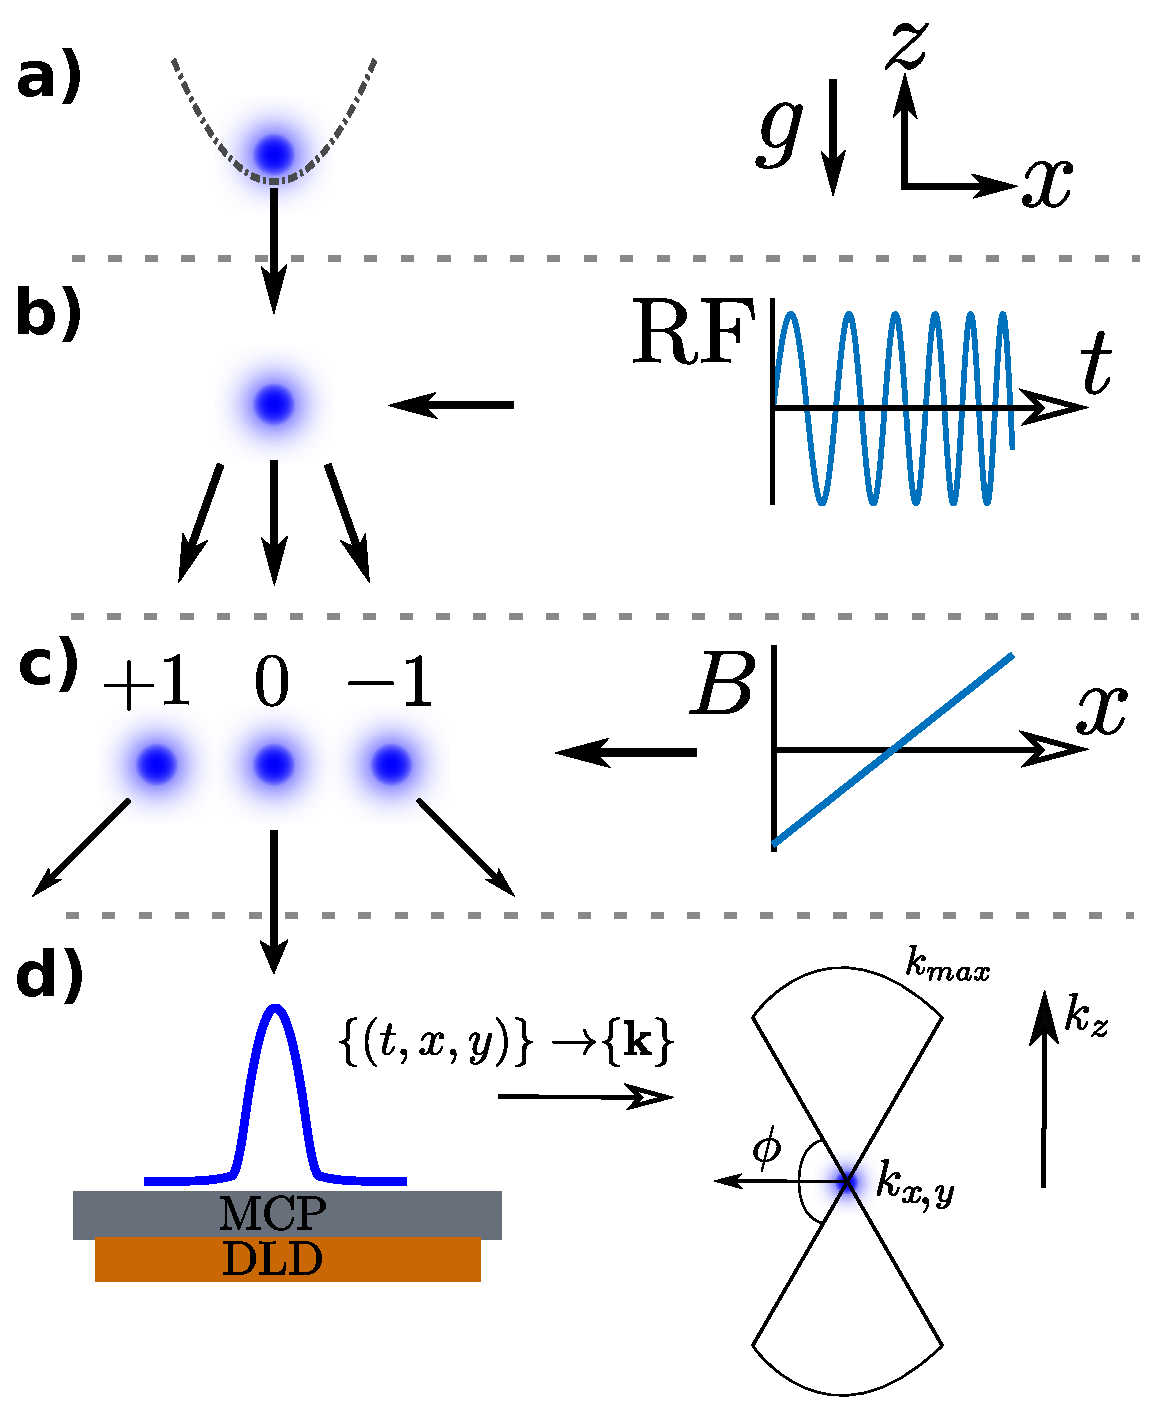
\includegraphics[width=0.4\textwidth]{fig/QD/exp_cartoon}
% %     \caption{Sketch of experimental sequence.
% 	A BEC is released from a harmonic trap (a) and expands during freefall before being split into a superposition of the $m_J\in\{-1,0,1\}$ states (b) by an RF chirp.
% 	A magnetic field gradient separates the clouds (c) ensuring that only the magnetically insentitive $m_J=0$ cloud lands on the detector (d), from which the momentum information is reconstructed.
% 	The quantum depletion lies in the dilute tails at large momentum (inset).}
% %     \label{fig:sequence}
% % \end{figure}


% % \begin{figure}[b]
% %         \includegraphics[width=0.5\textwidth]{fig/QD/contact_determination}
% %         \caption{The empirical density of particle momenta (a) for different peak densities, showing the transition between the condensed, thermal, and depletion regions (indicated for $n_0=20~\mu\textrm{m}^{3}$ with dotted lines).
% 	The number of atoms with wavevector $k\in\{k_1,k_2\}$ within the depletion region yields an estimate of the contact via Eqn.
% 	(\ref{eqn:c_est}).
% 	Fixing $k_2=10\mu\textrm{m}^{-1}$, we show $C_\textrm{est}$ as a function of the cutoff $k_1$ (b), which behaves consistently with a $k^{-4}$-like scaling of the momentum distribution.
% 	For each run we choose the $k_1$ at which $C_\textrm{est}$ is the most stable.}
% %         \label{fig:cdfplot}
% % \end{figure}

% % \section{Results} 
% % The single-particle detections can be used to construct an estimate of the far-field momentum density.
% 	However, estimating parameters of power-law distributions by fitting histograms is prone to bias and underestimation of uncertainties, especially when data is available over less than a decade of dynamic range \cite{clauset09,virkar14}.
% 	The preferred statistical tool for analysing power law distributions are maximum likelihood estimators \cite{goldstein04,clauset09,virkar14,hanel17}, but these are unavailable here because there are multiple sources of detection events, as detailed in \cite{SOM}.
% 	We present an approach that overcomes these issues, yielding the dependence of the tail amplitude on the condensate density in a straightforward way, along with a rigorous uncertainty estimate.
	

% % The Tan relations yield an expression for the asymptotic momentum density in terms of the \emph{contact} $\mathcal{C}$
% % \begin{equation}
% % \lim_{k\rightarrow\infty}\rho(k) = \frac{\mathcal{C}}{k^4}=\frac{64\pi^2a^2}{7} \frac{n_0 N_0}{k^4},
% % \label{eqn:mom_dist}
% % \end{equation}
% % where $n_0$ is the peak density of a condensate of $N_0$ atoms with s-wave scattering length $a$ \cite{tan08_energetics,tan08_momentum} (a detailed derivation is given in \cite{SOM}).
% 	Under the hypothesis that the \emph{in situ} depletion survives the expansion, one can integrate Eqn.
% 	(\ref{eqn:mom_dist}) to predict the expected number of atoms whose wavevector has a modulus in the interval $k\in (k_1, k_2)$, 

% % \begin{align}
% % \mathcal{N}_{k_1,k_2} &=\int_{k_1}^{k_2} \frac{\rho(k)}{(2\pi)^3}k^2~dk~d\theta~d\phi\\
% % 		&=\frac{\mathcal{C}}{2\pi^2}\left(\frac{1}{k_1}-\frac{1}{k_2}\right)
% % \label{eqn:pred_num}
% % \end{align}
% % where the $(2\pi)^3$ Jacobian ensures normalization in $k$-space.
% 	The inverse of Eqn.
% 	(\ref{eqn:pred_num}) thus yields an estimation of the tail amplitude (the contact)
% % \begin{equation}
% % C_\textrm{est} = \frac{2\pi^2N_{k_1,k_2}}{\eta}\cdot \frac{k_1 k_2 }{k_2-k_1},
% % \label{eqn:c_est}
% % \end{equation}
% % in terms the number of detected atoms $N_{k1,k2}$ and the total collection efficiency $\eta\approx0.3\%$, which accounts for the detector efficiency and geometric factors, as detailed in \cite{SOM}.
	

% % Fig.
% 	\ref{fig:cdfplot} (a) we show the empirical density $n(k)$ for three representative data collection runs.
% 	The three regimes of the condensate, thermal part, and depleted particles are visible, spanning over five orders of magnitude in density.
	

% % In Fig.
% 	\ref{fig:cdfplot} (b) we show the estimated contact $C_\textrm{est}$ as obtained from Eqn.
% 	(\ref{eqn:c_est}), as a function of the lower bound $k_1$ with $k_2=10~\micron^{-1}$.
% 	Indeed, Fig.
% 	\ref{fig:cdfplot} (b) and Eqn.
% 	(\ref{eqn:c_est}) provide a test for the presence of $k^{-4}$ scaling in the momentum density: Because Eqn.
% 	\ref{eqn:c_est} is derived assuming a $k^{-4}$ power law, any other behaviour would manifest as a clear dependence of $C_\textrm{est}$ on $k_1$.
% 	The invariance of $C_\textrm{est}$ in Fig.
% 	\ref{fig:cdfplot} therefore confirms the $k^{-4}$ power-law decay in the region of interest.
	

% % The value of $k_1$ must be determined for each run, as the crosssover over from thermal to quantum-depleted varies with the condensate density and temperature.
% 	We fix $k_1$ as the point where $dC_\textrm{est}/dk_1$ is minimized, ranging from $4.5-6.5\mu\textrm{m}^{-1}$ between runs.
% 	The uncertainty in the $C_\textrm{est}$ for each run is the standard error in the mean of $C_\textrm{est}$ over all the shots in that run.
% 	Across all runs, the average value of $C_\textrm{est}$ is 8(1) times \textit{in situ} predictions using Eqn.
% 	(\ref{eqn:pred_num}) and calibration parameters.
% 	The final uncertainty in this sensitivity is obtained by simple propagation of errors, avoiding the problem of total least-squares regression as encountered in the prior work \cite{chang16}.
% 	The empirical dependence of $C_\textrm{est}$ on the atom number and trapping frequencies is shown as a solid line in Fig.
% 	\ref{fig:results_comp}, with the uncertainty shown as a shaded area.
% 	Thus, while the observed momentum distribution is consistent with a $k^{-4}$ asymptotic decay, the amplitude of these tails contradicts the hypothesis of Eqn.
% 	(\ref{eqn:pred_num}) by 7$\sigma$.

    
% % 	\begin{figure}[t]
% % 	        \includegraphics[width=0.5\textwidth]{fig/QD/results_comp}
% % 	        \caption{Comparison of simulations and experiments.
% 	The inset is a zoomed view.
% 	 From our empirical data (ED) we determine the empirical contact $C_\textrm{est}$ which is linear in the product $N_0n_0$ (Eqn.
% 	(\ref{eqn:mom_dist})), but 8(1) times more sensitive (Av) than the prediction by the Tan theory (TT).
% 	The simulated contact of BECs in a cigar-shaped trap (CT) are consistent with (TT) before release and increases after expansion (CE), but by less than the experiment.
% 	A slow relaxation of the tight axes of the cigar trap (CS) leads to a reduction in the simulated contact.
% 	Simulations of a spherical trap (ST) show a negligible increase after expansion (SE).
% 	The prior \mhe result \cite{chang16} (IO) is shown for comparison (dashed line)}
% % 	        \label{fig:results_comp}
% % 	\end{figure}


% % 	\begin{figure}[b]
% % 	        \includegraphics[width=0.5\textwidth]{fig/QD/time_dep_theory}
% % 	        \caption{Simulations of condensates released from a cigar-shaped trap show an increase in contact after the trap release, stabilizing after a time on the order of $1/\omega_x$, several hundred $\mu$s.
% 	The relative difference between in-trap and expanded contact increases with the density of the condensate.
% 	For comparison, the experimental control pulses are implemented after 2ms of expansion.
% 	In contrast, when the transverse trapping frequencies are reduced by half (dotted line), the in-situ contact relaxes.}
% % 	        \label{fig:theory_time_dep}
% % 	\end{figure}
% % 	% \

% % 	\section{Simulations} To understand the excess contact here and in earlier experiments \cite{chang16}  
% % 	we performed simulations of the BEC expansion from harmonic traps using the first principles STAB method \cite{Deuar11,Kheruntsyan12}.
% 	The simulations included a cigar-shaped trap (marked CT in Fig.
% 	\ref{fig:results_comp}) with parameters matched to the experimental conditions (see \cite{SOM} for details).
% 	The in-trap state was consistent with the adiabatic sweep theorem before release from the trap.
% 	Following expansion from the cigar trap (CE), the simulated tail amplitude increased and stabilized at a factor of 1.64(9) above the predictions of Eqn.
% 	(\ref{eqn:mom_dist}).
% 	The steady-state occurs within a few hundred microseconds, much sooner than the 2ms delay between the trap release and application of the rf and Stern-Gerlach pulses.
% 	To understand the disagreement with earlier theory \cite{qu16}, which predicted no depletion survival, we also investigated the effect of adiabatic expansion on the in-trap depletion by simulating a slow decrease of the transverse trapping frequencies by a factor of two (CS), and found that the in-trap contact decreased roughly as predicted by Eqn.
% 	(\ref{eqn:mom_dist}) in these instances --- see the dashed line in Fig.~\ref{fig:theory_time_dep}.
% 	Details of the method and calculations are in supplementary material \cite{SOM}.
	

% % 	We interpret our results as an indication that the depleted atoms are accelerated by the non-uniform mean-field energy of the condensate during the expansion, and that this contributes to the disagreement between \emph{in situ} and measured contact.
% 	In detail, after a quench into the free particle regime, the condensate expands hydrodynamically on timescales of $1/\omega$.
% 	This is an adiabatic process for the low momentum depletion, whereby some depleted atoms are absorbed back into the condensate in agreement with \cite{qu16}.
% 	However, the characteristic time for reabsorption is $\hbar/gn_0$, slow enough that quasiparticles in the particle branch of the Bogoliubov dispersion have sufficient velocity to escape the expanding cloud without being reabsorbed and thus transition to free atoms.
	
	
% % 	Moreover, an atom inside the BEC experiences an effective force from the gradient of the mean-field potential $\textbf{F} = -4\pi\hbar^2a \nabla  n(x)/m$.
% 	This endows escaping depleted particles with a greater momentum, increasing the weight of the tails in the far-field.
% 	This effect is exacerbate in light atoms like $^{4}$He: because the acceleration scales with $1/m^2$, it would be suppressed by a $\sim500$-fold in $^{87}$Rb experiments \cite{makotyn14}.
% 	This picture is supported by our simulations, in which we observe a decrease in the total number of depleted particles (reabsorption) and a simultaneous increase of the large-k population (forcing).
% 	Further, it is much easier for depletion atoms to escape and be accelerated in the transverse x-y directions from an elongated cloud because the distances $R_{TF}=\frac{1}{\omega}\sqrt{2gn_0/m}$ are reduced by $\bar{\omega}/\omega_{x,y}$, whereas the initial mean depletion velocities \textit{in situ} $v\sim \sqrt{2gn_0/m}$ are isotropic: Indeed, spherical clouds (SE) exhibit a much weaker effect than the elongated clouds (CE) owing to the longer escape time.
	 

% % 	\section{Discussion} 
% % 	Our work expands the growing suite of far-field investigations of quantum depletion \cite{cayla20,chang16} and confirms that quantum depletion can, remarkably, survive past the lifetime of its original condensate.
% 	Our findings clarify that how the depletion can be visible in the far-field momentum distribution here and in earlier experiments, and that the hydrodynamic approximation does not capture sufficient short-wavelength information to make detailed predictions about the high-momentum behaviour.
% 	We thus find a partial explanation for the deviation of the far-field distribution from both the predicted in-situ depletion and the hydrodynamic reabsorption: The interplay between coherent absorption of Bogoliubov excitations and the dispersal of the chemical potential into kinetic energy, to which helium is particularly sensitive, result in a growth of the $k^{-4}$ tails of the momentum distribution during freefall.
% 	However, a mystery remains: Why is the excess depletion some four times greater than accounted for by this picture? This issue should be resolved in order to interpret far-field observations in terms of the in-trap physics of interest.
% 	This question invites complementary studies of the \emph{in situ} depletion in \mhe BECs.
% 	The important question of whether the far-field anomaly originates in the trapped state or during expansion would be best pursued with Bragg spectroscopy, given the complications of radio spectroscopy of Helium as discussed in \cite{SOM}.


% % \section{Detection}

% % 	We use a Roentdek DLD80 multichannel plate and delay-line detector stack \cite{Manning10} with a quantum efficiency of $\approx8\%$, and space and time resolutions of 100 $\mu$m and 3 $\mu$s, respectively \cite{Henson18}.
% 	After the atoms are released from the trap, they fall 859mm to the detector stack, which registers the arrival times and positions $(t_i,x_i,y_i)$ of each atom, indexed by $i$.
% 	The centre of mass of the cloud arrives after a $\tau = 417$ms time of flight following the trap switch-off.
% 	The velocity of each atom relative to the centre of mass of the cloud is given by $(v_x,v_y,v_z) = t_{i}^{-1}(x_i-\bar{x},y_i-\bar{y},g_0(\tau^2-t_{i}^{2}))$, where $g_0$ is the local gravitational acceleration and the overbar denotes the within-shot average.
% 	The velocity conversion assumes a point source but carries a negligible error of a few ppm as the in-trap BEC size is smaller than the detector resolution.
% 	We centre the counts from each realization and detection sequence (termed a \emph{shot}) and transform the counts from cartesian velocity space to spherical polar coordinates with radius $k$ (in $m^{-1}$), polar angle $\theta$ and elevation angle $\phi$, relative to the centre of the cloud, where the velocity-to-wavevector transformation follows from  $\textbf{p}=m\textbf{v}=\hbar\textbf{k}$.
	



% % 	The detector efficiency was $\chi=0.08(2)$, as we determined from the collection efficiency of correlated atoms on the opposite sides of scattering halos \cite{shin19,shin20,Jaskula10}.
% 	The solid angle in k-space available to detect the depleted tails is limited by the 40mm radius of the circular detection surface.
% 	The field of view of our detector in the $(x,y)$ plane is $\lesssim5\times 10^6$ m$^{-1}$, which is only just sufficient to reach past the edge of the thermal region.
% 	Therefore, we sample data from the segments of the sphere with elevation angle $|\phi|>\pi/3$ rad and $|k|<10^7$ m$^{-1}$, centred on the BEC, which encompasses a total solid angle of $0.13\times 4\pi$ steradians.
% 	The noise floor is set by the detector's dark count rate of $0.56(1)$ Hz cm$^{-2}$, which contributes an average of 0.4(2) counts to the region of interest (ROI) per shot.
% 	 A summary of the results for each data run are shown in Tab.
% 	\ref{tab:results}.






% % % \todo{Density plots out to larger $|k|$ to show descent into noise floor? How far could we push it until we hit dark counts?}

% % % \section{Spin mixing}
% % % Also lets us determine thermal fraction - note it isn't determinable from the PAL because of the mean-field broadening (but one could just make fits and subtract the thermal part, yes?).
% 	I think the mean-field expansion is particularly bad for Helium, and wasn't reported much before, because we are 5% the mass of popular species like Rb so much more subject to mean-field acceleration!

% % \section{Trap configuration and calibration}

% % 	We prepared our BECs with via forced evaporative cooling in a harmonic magnetic trap with trap frequencies $(425,425,45)$ Hz and a DC bias stabilized by our auxiliary field compensation coils \cite{Dall07,Dedman07}.
% 	For the tight trap we increased the coil current after the cooling sequence to obtain trapping frequencies $(902,895,71)$ Hz, ramping the field as a sigmoid step function to minimize in-trap oscillations.
% 	The trap remained on for 150ms before switching the trap off with a $1/e$ time of $\approx38\mu$s.
% 	The condensates were allowed to expand for 2ms before we transferred some of the condensate into the magnetically insensitive $m_J=0$ state via Landau-Zener sweep to prevent distortion by stray magnetic fields.
% 	The RF pulse was created by a  function generator, amplified, and applied to the experiment chamber by a coiled antenna inserted into the BiQUIC coil housing.
% 	The pulse swept from 1.6-2.6MHz over 1ms and was centred on the fine structure resonance between the $m_J$ states.
% 	The transfer efficiencies $\eta_j$ for each of the $m_J = j$ states is discussed in the next section.
% 	The sweep was $10^6$-fold wider than the Doppler broadening of the BEC which ensured uniform transfer at all momenta.
% 	Immediately after the RF sweep, the bias coils are switched off and auxiliary push coils in the vertical (Z) and weak horizontal (X) axes are activated using a fast MOSFET switch to implement a Stern-Gerlach separation of the $m_J = -1,~0,$ and $+1$ pulses.

% % \subsection{Determining transfer efficiency}

% % 	To calibrate the transfer efficiencies, we applied a weaker Stern-Gerlach than for the depletion measurement, resolving each $m_J$ cloud on the detector, as illustrated in Fig.
% 	\ref{fig:frac_cal}.
	

% % \begin{figure*}[!t]
% % 	\begin{center}
% % 		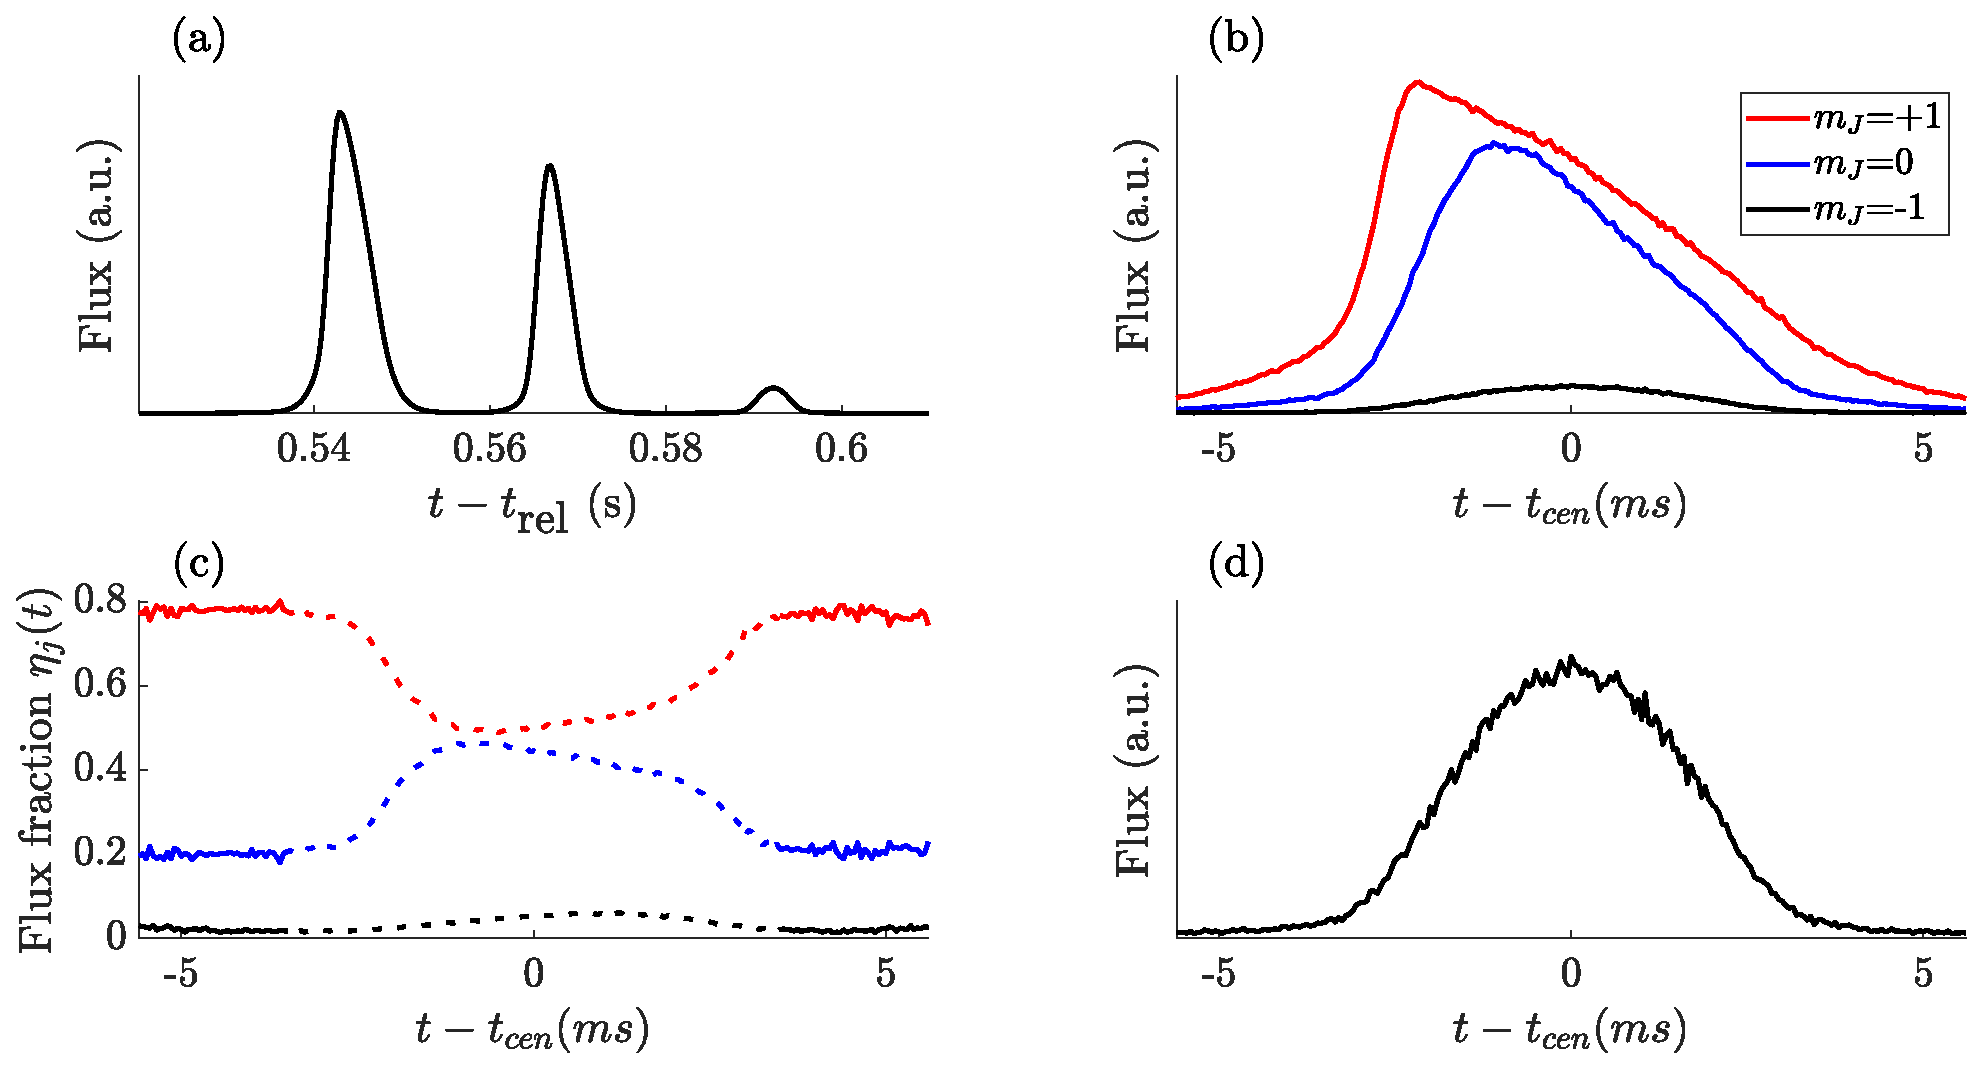
\includegraphics[width=\textwidth]{fig/QD/frac_cal_profile}
% % 		\caption{Determining the RF transfer efficiency.
% 	The time-of-flight profiles of each pulse are resolved (a) by applying a weak Stern-Gerlach pulse during the time of flight.
% 	The pulses are aligned with respect their centre-of-mass (b) and used to determine the pointwise fraction ((c), dotted line).
% 	Detector saturation is evident in the peaks (dashed lines), but not in the thermal tails (solid lines), which are used to compute the transfer efficiency.
% 	Because of its lower flux, the $m_J=-1$ pulse does not show evidence of saturation (d) and is used to determine the thermal fraction.}
% % 		\label{fig:frac_cal}
% % 	\end{center}
% % 	\end{figure*}

% % 	The efficiencies $\eta_J$ cannot be calculated by counting the atoms in each cloud because the detector saturates during the peak condensate flux, but we can compare the thermal parts.
% 	We align each cloud along the time (Z) axis and compute the pointwise fraction of the atomic flux $\phi(t)$ accounted for by each cloud, $\eta_j(t) = \phi_j(t)/\sum_j\phi_j(t)$, as depicted in Fig.
% 	\ref{fig:frac_cal}.
% 	The ratio of densities between the clouds is roughly constant in the thermal part, indicating the absence of important saturation effects and a spin transfer that is independent of $k$.
% 	The fraction of the original cloud transferred into each $m_J$ state is determined by taking the average $\langle\eta_j(t)\rangle$ over the thermal tails.
% 	We find these efficiencies are approximately 74\%, 24\%, and 2\% in all runs for the $m_J=+1$, 0, and -1 states, respectively.
	
% % 	While the $m_J=0$ and $m_J=1$ clouds clearly saturate the detector, the small fraction ($\approx2\%$) of the atoms transferred to the $m_J=-1$ state does not (Fig.
% 	\ref{fig:frac_cal} (d)).
% 	A bimodal fit to the condensed and thermal parts, plus constant background, yields an estimate of the thermal and condensed fractions.
	


% % % \subsection{Determination of thermal fraction}
	

% % % 	\begin{figure}[!h]
% % % 	\begin{center}
% % % 		\includegraphics[width=0.8\textwidth]{fig/QD/m1_frac_anal}
% % % 		\caption{Comparison of thermal fits in the unsaturated $m_J=-1$ pulse including 138 shots.
% 	The weak (X) and strong horizontal (Y) trapping axes are shown in (a) and (b), respectively.
% 	\org{would be helpful to label $v_x$ and $v_y$ to make it self-evident at 1st glance.} Both projections display a bimodal peak, with the condensate (dotted lines) and thermal parts (thick solid lines) easily distinguished.
% 	Fitting a Gaussian profile (thin solid line) to the velocity distribution of the thermal part yields the thermal number and temperature.
% 	Subtracting the fit leaves the condensate profile (c) which can be \blu{\dots something\dots} yields the condensed number.}
% % % 		\label{fig:thermal_frac}
% % % 	\end{center}
% % % 	\end{figure}



% % \subsection{Analysis of spin transfer measurements}

% % 	In early tests of our measurement sequence we noticed a contamination of the signal by spurious counts.
% 	We inferred these were remnant counts from the $m_J=+1$ cloud as they were still visible when we ran an experimental sequence without the Landau-Zener transfer.
% 	This contamination appeared in a particular region of our detection image, illustrated in Fig.
% 	\ref{fig:spinpop}.
% 	As such we were able to correct for it by subtracting their contribution from the counts collected during measurement shots.
% 	Generally, fewer atoms can be attributed to this noise than would be required to explain the discrepancy described in the main text, as illustrated in Fig.
% 	\ref{fig:num_counts}.
% 	While the cause of the cross-contamination is unclear, we observe that the count density outside the region of interest is similar in both the shots with the RF pulse and those without.
% 	We hypothesize that the remnant counts are atoms transferred into the $m_J=0$ state by non-ideal behaviour of the Stern-Gerlach pulses.
	

% % 	As mentioned in the main text, the presence of these counts also prevents a straightforward application of a maximum-likelihood estimator (MLE) to determine parameters of the power-law region.
% 	The basic principle of the MLE is to assume a functional form for the probability distribution $p(x|\theta)$ underlying the observed data $x$, and dependent on some parameters $\theta$; the zero of the derivative of the \emph{likelihood} function $L(\theta|x)$ with respect to the parameters $\theta$ then yields the most-probable parameter values given a set of observations $x$.
% 	In our context, one can assume a functional form for the probability distribution underlying atomic detection events (via a wavefunction ansatz).
% 	The detector dark count rates can also be incorporated by assuming a uniform distribution.
% 	Such an analytical treatment does not readily permit the inclusion of an empirical density estimate which itself includes the aforementioned dark count rate.
% 	Instead, we opt for the simpler approach described in the main text.

% %     \begin{figure}[!b]
% % 	\begin{center}
% % 		\includegraphics[width=\columnwidth]{fig/QD/spinpop}
% % 		\caption{Measured contribution of the detector dark counts and spurious spin counts to the time-of-flight profile.
% 	We accounted for the pulse at around 550ms and subtracted it from the measured profiles when computing the contact.
% 	After removing this background term, the density profiles above and below the condensate agree, indicating convergence on the true signal.
% 	For reference, the peak flux of the $m_J=0$ condensate is about a thousandfold greater than the peak shown here.}
% % 		\label{fig:spinpop}
% % 	\end{center}
% % 	\end{figure}

% % 	% \begin{figure}[!h]
% % 	% \begin{center}
% % 	% 	\includegraphics[width=\textwidth]{fig/QD/profile_overlay}
% % 	% 	\caption{Comparison of average time-of-flight profiles over a single data run for the quantum depletion measurement shots (blue, 871 shots), transfer efficiency calibration (black, 112 shots), detector dark counts (red, 871 shots), and spurious counts (dot-dash, 895 shots).
% 	The time window bounded by $|k|\leq 10\mu$m is indicated with dotted lines.
% 	Shaded area is the standard error over the entire run.}
% % 	% 	\label{fig:tof_profile}
% % 	% \end{center}
% % 	% \end{figure}




% % % Note that the temps disagree between axes, but within axes between clouds they are consistent(....ish).
% 	This means we can use the profile ratio method, which is also consistent with comparing the thermal number from the fits.
% % % Perhaps comment on the thermal-subtracted part; the TF profile should have a sharp cutoff, but the smooth edges are suggestive evidence of this roll-off

% % \begin{figure}
% % 	\centering
% % 	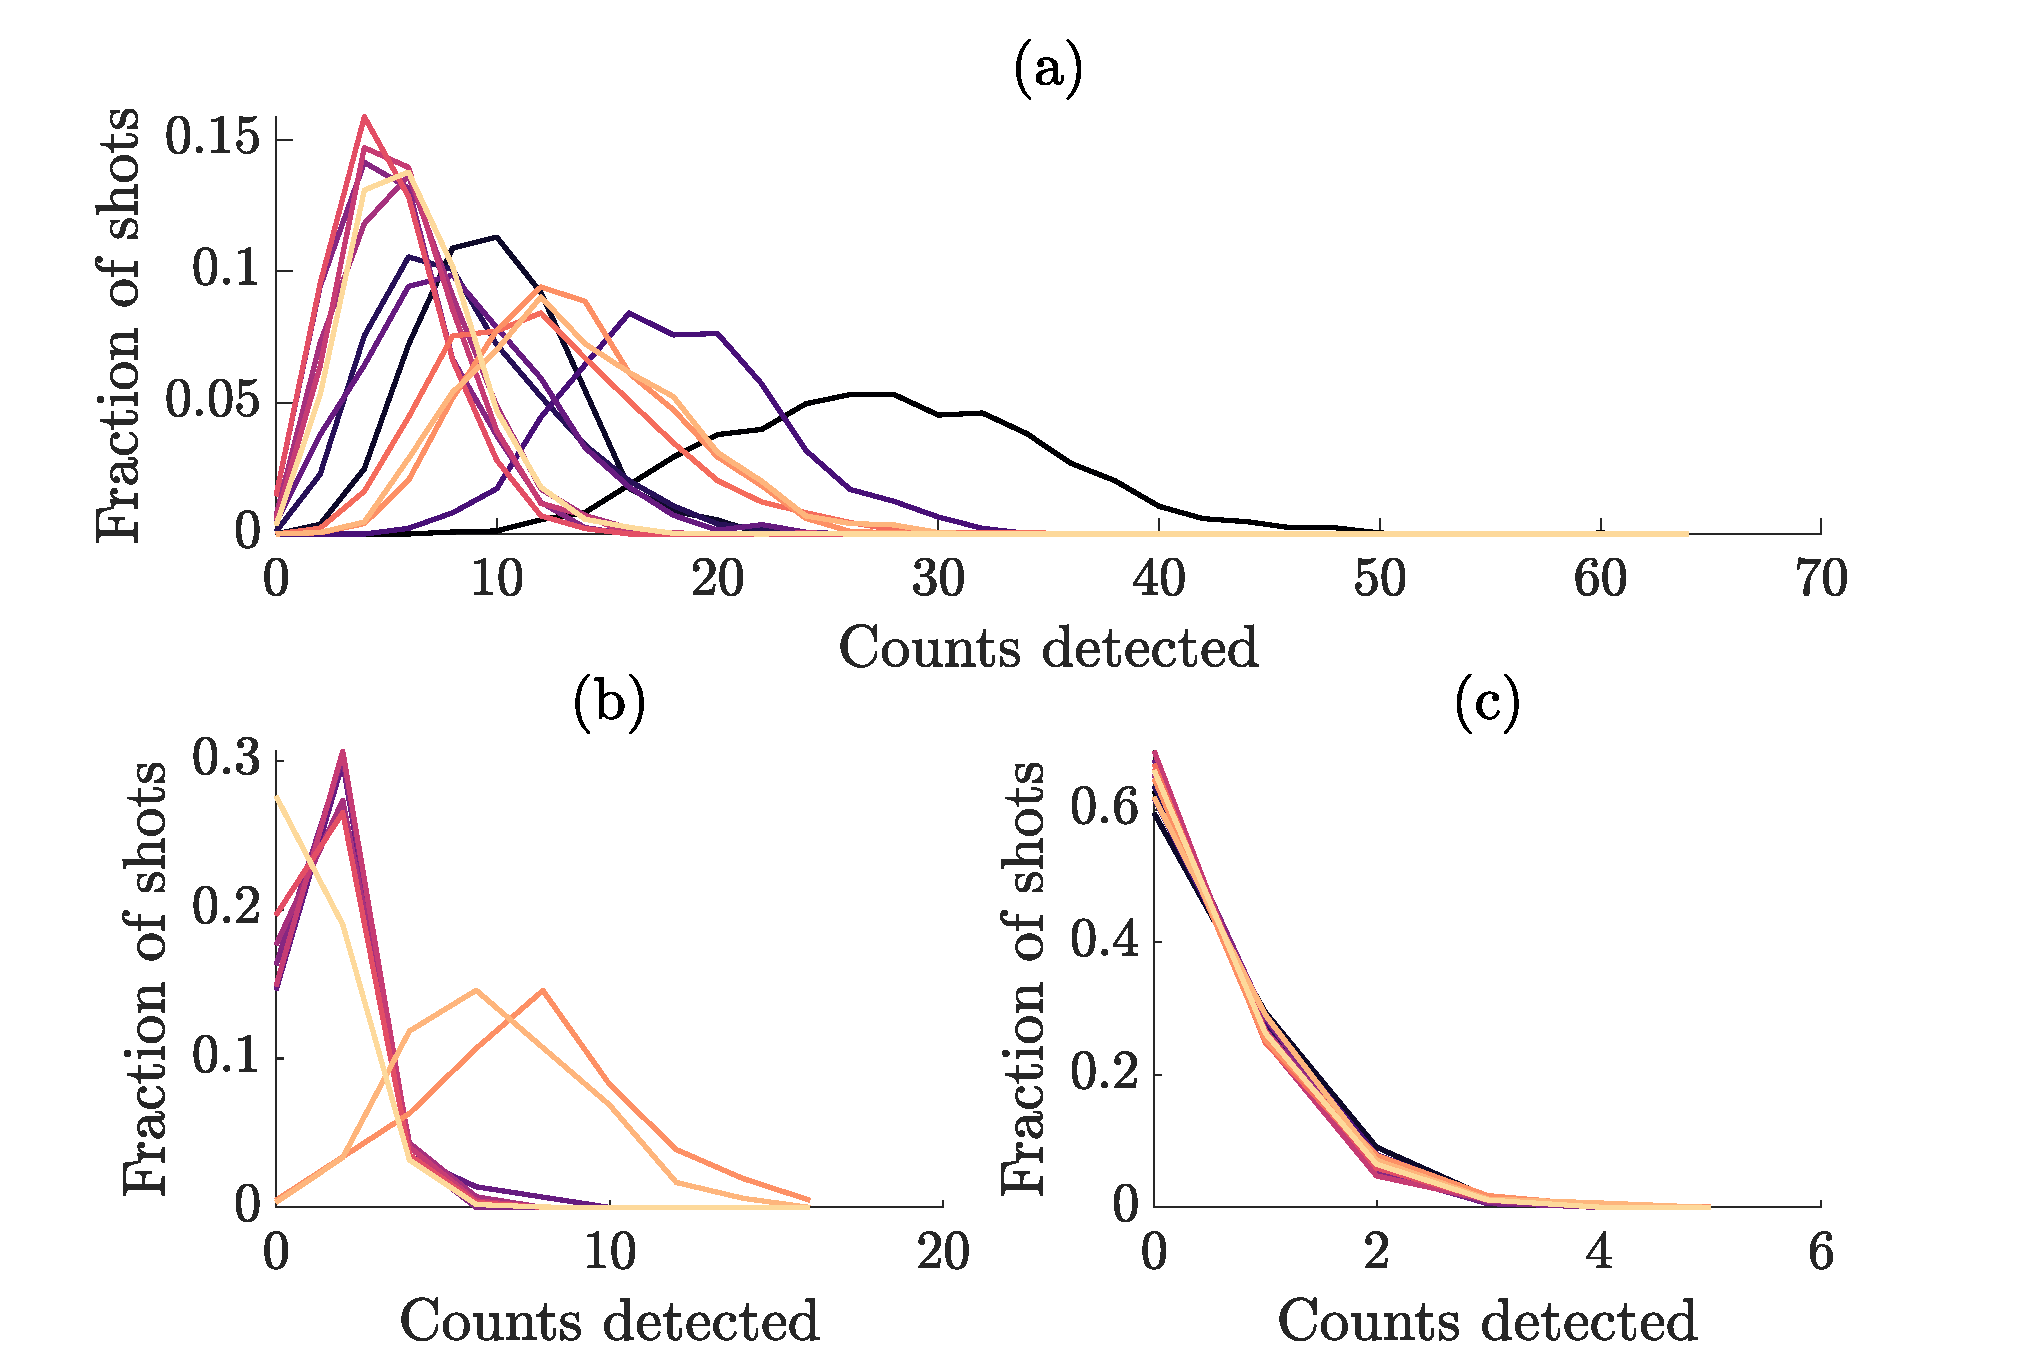
\includegraphics[width=0.5\textwidth]{fig/QD/counts_per_run}
% % 	\caption{Number of counts detected in the region of interest in the depletion measurement (a), the spin mixing calibration (b), and the dark count calibration (c).
% 	An average of 3.0(5) counts were detected in the ROI in the spin-mixing calibration shot, and the background count rate was 0.4(2) counts per shot.
% 	Separate lines indicate separate \emph{runs}, i.e.
% 	sequences of shots with fixed parameters.}
% % 	\label{fig:num_counts}
% % \end{figure}


% % \subsection{Peak density calibration}

% %     The quantum depletion and contact are both predicted to depend solely on the condensed number and trapping frequencies via the condensate density, hence it is important to determine both quantities accurately.
% 	In the Thomas-Fermi approximation, the peak density of the condensate can be written as $n_0 = \mu/g$, where $\mu$ is the chemical potential, $g=4\pi\hbar^2a_{1,1}/m$ is the effective interaction strength, $m\approx6.6\times10^{-27}$ kg is the atomic mass, and $a=7.512$ nm is the s-wave scattering length between pairs of atoms in the $m_J=1$ state \cite{Moal06}.
% 	The expression for the peak density can be expanded as
% % 	\begin{equation}
% % 		n_0 = \frac{1}{8 \pi}\left( (15N_0)^2 \left(\frac{m \bar{\omega}}{\sqrt{a_{1,1}} \hbar}\right)	 ^{6}\right)^{1/5}
% % 		\label{eqn:n0}
% % 	\end{equation}
% % 	where $\bar{\omega} = \left(\omega_x\cdot\omega_y\cdot\omega_z\right)^{1/3}$ is the geometric trap frequency and $N_0$ is the number of atoms in the condensate.
% 	During these calibration runs we simultaneously determine the total atom number $N$ and trap frequency $\bar{\omega}$ in a single shot using a pulsed atom laser and use the thermal fraction to determine the condensed number $N_0$.
	

% % 	The pulsed atom laser consists of a series of Fourier-broadened RF pulses centred on the minimum Zeeman splitting in the trap.
% 	The pulse transfers atoms in the trap to the untrapped $m_J=0$ state with an approximately constant transfer rate across the cloud.
% 	We outcouple approximately 2\% of the atoms per 100$\mu$s pulse for $\approx$200 pulses, which eventually depletes the entire trap.
% 	The atom laser thus prevents the detector from saturating and allows an accurate determination of the atom number, up to a factor of the quantum efficiency.
% 	We determine the trapping frequencies by inducing centre-of-mass oscillations with a magnetic impulse, and finding the oscillation period from the atom laser pulses \cite{henson18ML}.

% % % 	\begin{figure}[!h]
% % % 	\centering
% % % 		\includegraphics[width=0.8\textwidth]{fig/QD/pal_shot}
% % % 		\caption{A kicked pulsed atom laser with motion sampled at 11ms intervals.
% 	The oscillations in the centre-of-mass position of each pulse are shown along the Y axis over time (a).
% 	The apparent frequency can be determined for each axis (b).
% 	The outcoupling efficiency is fixed throughout the sampling sequence (c), producing a geometric decay of the number of atoms in each pulse.
% 	The straight line on a logarithmic scale shows that detector saturation saturation is negligible and that the BEC population does not affect the transfer rate.}
% % % 		\label{fig:pal_shot}
% % % 	\end{figure}
	
% % % \subsection{Measuring the trapping frequencies}

% % % 	To illustrate how we obtain the trapping frequencies, consider an undamped harmonic oscillator in one dimension.
% 	The centre-of-mass momentum $p(t) = A \cos(2\pi f t))$ oscillates at a frequency $f$ Hz, and the centre of mass of a pulse outcoupled at time $t'$ lands on the detector at a position $x'(t+\tau) = p(t')\tau/m$, where $\tau$ is the time of flight of the centre of mass.
% 	Sampling the cloud motion with a sampling period T starting at initial time $t_0$ produces a series of pulses whose centres of mass land at $\{x_n = (A\tau/m) \cos(\omega(t_0+nT))\}$.
% 	The sampling frequency $f_s=1/T$ determines the \emph{Nyquist frequency} $f_N=f_s/2$, which is the maximum frequency that can be reconstructed unambiguously from such a sampling regime.
% 	When $f>f_N$ the signal manifests as a lower-frequency oscillation known as the \emph{alias} of the signal.
% 	The aliased frequency $f_a$ is

% % % 	\begin{equation}
% % % 	 f_a =
% % % 	  \begin{cases}
% % % 	   \frac{Z_n f_s}{2} - f & \text{if } Z_n \text{ even} \\
% % % 	   f - \frac{(Z_n-1)f_s}{2}       & \text{if } Z_n \text{ odd},
% % % 	  \end{cases}
% % % 	  \label{eqn:Z_N}
% % % 	\end{equation}
	
% % % 	where $Z_n = \lceil{f/f_N}\rceil$ is the Nyquist zone number, as described in numerous RF engineering references.\org{Indeed ;-) probably needs rephrasing though}.
% 	While it is not possible to determine $Z_N$ for a signal with an unknown (not necessarily stationary) $f$ from samples taken at a fixed $f_s$, one can vary $f_s$ and determine both $Z_N$ and $f$ from the gradient $d f_a / d f_s$.
	
% % % \begin{figure}[!h]
% % % 	\centering
% % % 		\includegraphics[width=0.8\textwidth]{fig/QD/sawtooth_plot}
% % % 		\caption{Aliasing of the trap frequency oscillations under different sampling regimes.
% 	The fitted oscillation frequency is shown in each axis for a range of sampling frequencies.
% 	The sawtooth function is a one-parameter fit which determines the underlying frequency of the centre-of-mass oscillations.}
% % % 		\label{fig:sawtooth_plot}
% % % 	\end{figure}	

% % % 	We induce oscillations of the BEC in all three axes by briefly displacing the trap centre with a perturbation to the trapping field.
% 	The maximum sampling frequency is limited by the temporal width of the BEC pulse landing on the detector to about 100Hz, yielding a Nyquist frequency too low to resolve the un-aliased oscillations.
% 	We fit the apparent oscillation frequency in each axis as a function of sampling frequency as shown in Fig.
% 	\ref{fig:sawtooth_plot}, along with a one-parameter fit of Eqn.
% 	\ref{eqn:Z_N}.
% 	\blu{We thus} determine that the frequencies $(\omega_x,\omega_y,\omega_z)$ of each of the traps used in the experiment are $2\pi\times(45,425,425)$ and $2\pi\times(72,889,893)$, respectively, which are stable to within 5\% throughout the duration of the data collection and to better than $1\%$ in a given run.


% % \begin{table*}
% % 	\begin{tabular}{c c c c c c c}
% % 	\hline\hline
% % 	Peak density ($\micron^{-3}$) & $N_\textrm{tot}$ ($\times10^5$) & Thermal fraction & $N_\textrm{Detect}$ & $N_\textrm{pred}$ & $C_\textrm{est}$ (pm$^{-1}$)  &$C_\textrm{est}/\mathcal{C}$  \\ 
% % 	\hline 
% % 	16(1) & 3.5(4) & 0.09 & 5.6(0) & 0.7(1) & .2(1)& 7(3) \\ 
% % 	18(1) & 5.0(4) & 0.17 & 6.8(1) & 0.9(2) & .2(1)& 7(2) \\ 
% % 	19(2) & 4.9(6) & 0.08 & 8.1(1) & 1.0(2) & .3(1)& 7(3) \\ 
% % 	20(1) & 5.7(3) & 0.09 & 14.(1) & 1.3(3) & .5(1)& 10(3) \\ 
% % 	38(2) & 3.9(3) & 0.14 & 4.9(0) & 0.4(1) & .6(3)& 10(5) \\ 
% % 	38(3) & 3.7(4) & 0.09 & 3.5(0) & 0.4(1) & .4(2)& 7(4) \\ 
% % 	38(3) & 3.8(4) & 0.11 & 3.7(1) & 0.6(1) & .4(2)& 6(3) \\ 
% % 	38(3) & 3.7(4) & 0.09 & 4.1(0) & 0.5(1) & .5(2)& 7(4) \\ 
% % 	39(4) & 3.8(5) & 0.10 & 4.3(0) & 0.5(1) & .5(3)& 7(4) \\ 
% % 	41(2) & 4.5(4) & 0.12 & 6.5(1) & 0.6(1) & .8(4)& 9(5) \\ 
% % 	\hline\hline
% % 	\end{tabular}
% % 	\caption{Summary of results for each data run.
% 	The peak density is determined from measurements of the condensed number (via the total number $N_\textrm{tot}$ and condensate fraction) and trapping frequencies, which in turn is used to predict the contact $\mathcal{C}$.
% 	The number $N_\textrm{Detect}$ of atoms detected in the region of interest can be used to determine the empricial contact $C_\textrm{est}$ from the $k^{-4}$-like tail, as in the main text, and can be compared to the predicted number of counts $N_\textrm{pred}$.
% 	The final column shows the ratio of the estimated to predicted contact, also equal to the ratio of the detected and predicted counts.}
% % 	\label{tab:results}
% % \end{table*}

% % \section{Theory}

% % The Hamiltonian of a homogeneous system of interacting bosons, with plane-wave field operators $\hat{a_\kvec}$ labeled by the wavevector $\kvec=\textbf{p}/\hbar$, can be diagonalized by the Bogoliubov transformation to a free Bose gas of collective excitations with operators $\hat{b}_\kvec$ \cite{Bogolubov47}.
% 	This permits the single-particle momentum density to be written as $\rho(k) = \langle\hat{a}_\kvec^\dagger\hat{a}_\kvec\rangle=\left(u_{\kvec}^{2}+v_{\kvec}^{2}\right)\langle b_{\kvec}^{\dagger}b_{\kvec}\rangle + v_{\kvec}^{2}$, where $\hat{a}_\kvec = u_\kvec \hat{b}_\kvec + v_{-\kvec}\hat{b}^\dagger_\kvec$, $\hat{a}^\dagger_\kvec = v_\kvec \hat{b}_\kvec + u_{-\kvec}\hat{b}^\dagger_\kvec$ and the $u_\kvec$ and $v_\kvec$ terms are fixed by the condensate density, atomic mass, and s-wave scattering length \cite{PitaevskiiStringari,PethickSmith}.
% 	In the ground state, devoid of thermal excitations, the quasiparticle modes are populated by the $v_{\kvec}^{2}$ term \cite{decamp18,chang16}.

% % While the local-density approximation (LDA) can be employed to compute the amplitude of the $k^{-4}$ tail using the Bogoliubov disperson \cite{chang16}, the approach opened by Tan's original theorems is simpler than integrating $v_\kvec^2$ across a Thomas-Fermi distribution.
% 	The two-body contact is defined by \cite{tan08_momentum}
% % \begin{equation}
% % \mathcal{C} = \lim_{k\rightarrow\infty}k^4\rho(k),
% % \label{eqn:MomentumDef}
% % \end{equation}
% % where the contact $\mathcal{C}$ is the volume average of the local \emph{contact intensity} $\hat{C} = 32 \pi^2 a^2 \hat{n}^2$ \cite{werner12_boson}.
% 	The contact is related to the total energy $E$ through the \emph{adiabatic sweep theorem} \cite{tan08_energetics},
% % \begin{equation}
% % \mathcal{C} = \frac{8\pi m a^2}{\hbar^2}\frac{\partial E}{\partial a},
% % \end{equation}
% % where $a$ is the s-wave scattering length.
% 	In the Thomas-Fermi approximation, the energy per particle of $N_0$ condensed bosonic atoms is 
% % \begin{equation}
% % \frac{E}{N_0} = \frac{5}{7}\mu = \frac{5}{7} \frac{\hbar \bar{\omega}}{2} \left(\frac{15 N_0 a}{a_\textrm{HO}}\right)^{2/5},
% % \label{mu}
% % \end{equation}
% % where $a_\textrm{HO} = \sqrt{\hbar/(m \bar{\omega})}$ is the harmonic oscillator length and $\bar{\omega}=\sqrt[\uproot{2}\scriptstyle 3]{\omega_x \omega_y \omega_z}$ is the geometric trapping frequency \cite{PitaevskiiStringari,PethickSmith}.
% 	The sweep theorem yields
% % \begin{equation}
% % \mathcal{C} = \frac{8\pi}{7} \left(15^{2}(a N_0)^{7} \left(\frac{m \bar{\omega}}{\hbar}\right)^{6}\right)^{1/5},
% % \label{eqn:TotalHarmonicContact}
% % \end{equation}
% % which shares many factors with the peak density of a harmonically trapped condensate (Eqn.
% 	\ref{eqn:n0}), whereby one has
% % \begin{equation}
% % 	\frac{\mathcal{C}}{n_0} = \frac{64\pi^2a^2}{7} N_0.
% % \end{equation}

% % By substitution into Eqn.
% 	(\ref{eqn:MomentumDef}) one arrives at the expression

% % \begin{equation}
% % \rho(k) = \frac{64\pi^2a^2}{7} \frac{N_0n_0}{k^4}
% % \end{equation}

% % Higher-order effects are negligible in our experiments.
% 	The Lee-Huang-Yang (LHY) corrected condensate energy $E'$ for a uniform condensate with density $n$ yields an estimate of the worst-case contribution
% % $$
% % \frac{\partial E'}{\partial a} = \mathcal{C}\left(1+\frac{64\sqrt{na^{3}}}{3\sqrt{\pi}}\right),
% % $$
% % Where $\mathcal{C}$ is the contact computed neglecting the LHY term, and the second term in brackets is the LHY correction which amounts to at most a correction of order 1\%, using the highest $n_0$ observed in our experiments.
% 	In reality the correction will be smaller as the density is not uniform and is bounded above by $n_0$.


% % \subsection{Radio spectroscopic prospects}
% % The cause of the contact anomaly could be elucidated by determining whether it originates in the trapped condensate, or is generated during the trap release and expansion.
% 	Such an investigation requires an \emph{in situ} probe of the contact, such as the radio and Bragg spectroscopic techniques.
% 	The latter may be the most fruitful of the two simply because of the difficulty of interpreting the results from the former, which we sketch below.
% 	The basic principle of RF contact spectroscopy is to apply a monochromatic RF probe which is detuned from the resonance between two spin states, coupling atoms in the initial spin state to an untrapped channel, and then perform a differential measurement of the atom number.
% 	The signal strength scales with the difference of reciprocal scattering lengths $\Gamma\propto(1/a_\textrm{i,i}-1/a_\textrm{i,f})$ between pairs of atoms in initial-initial ($a_{i,i}$) and initial-final ($a_{i,f}$) spin states \cite{braaten10,wild12}, which can be manipulated via Feshbach resonance to obtain a good signal.
% 	For He$^*$ (spin 1) however, the scattering lengths $a_{1,1}$ and $a_{1,0}$ are identical \cite{Leo01}, rendering the preferred $m_J=1-m_J=0$ transition unusable.
% 	On the other hand, $a_{1,-1} = 3/7 a_{1,1}$ \cite{vassen16}, and the singlet transition can be driven without populating the $m_J=0$ state.
% 	In principle this could produce a detectable flux of atoms to perform sensitive in-trap contact measurements, however, collisions in the $^1\Sigma_{g}^{+}$ channel have large Penning ionization rates which lead to significant trap losses \cite{Leo01}.
% 	The ionization products would be detectable by in-vacuum channel electron multipliers but require theoretical work to disentangle from the spectroscopic signal.
% 	Further, such an experiment could not take advantage of a Feshbach resonance to increase signal strength or decrease the ionization rate.
% 	While such a measurement is not \emph{prima facie} impossible, Bragg spectroscopy may yield more comprehensible results.

% % % ? See Pitaevskii Stringari p34 for expressions for the Bogoliubov coefficients; can plug in the dispersion relation and show the asymptotic behaviour for uniform system at least
% % % Healing length defines the phonon-particle crossover - where does this sit wrt the depletion and thermal parts?
% % % Look into beliaev decay again, be more specific about mechanism
% % % Have the Bogo transform the wrong way around!!!

% % \section{Abstract}
% % A recent measurement of Tan's contact \cite{chang16} exceeded predictions based on the characteristics of the trapped condensates, in contrast to arguments that the dilute tails of the momentum distribution should vanish in the far-field.
% 	We measure Tan's contact in another laboratory and apply a distinct analysis method.
% 	The high-$k$ tails are visible and consistent with a $k^{-4}$ decay, and larger than a straightforward prediction, but the difference is less than that of the prior work.
% 	Our data and simulations of the expansion dynamics indicate that mean-field interactions between condensed and quantum depleted atoms are significant in the early expansion following release from the trap.
% % % max 600chars for PRL
% % % 597chars including spaces...
	


% % % See Mewes97 for analysis of landau-zener sweep in three-level system

% % % \maketitle

% % % 3,750 word limit !!

% % \section{Introduction} 
% % % Need better hook, cf "A fundamental question raised by the observation of natural systems is how macroscopic and collective properties depend on microscopic few-body interactions"
% % The controlled realization of quantum degenerate systems is a triumph of  both engineering and abstract models of matter.
% 	A modern supplement to the theories of quantum matter, the \emph{contact}, \cite{tan08_energetics,tan08_momentum,tan08_virial} links several universal relations between many-body features and microscopic information in aribitrary spin mixures at any density, temperature, and geometry \cite{combescot09,braaten08,braaten11,werner12_boson,werner12_fermion}.
% 	Originally formulated for low-energy scattering in the s-wave regime, emerging evidence for analogous relations in p-wave scattering \cite{luciuk16} hints at the existence of new systematic ways to connect and control thermodynamic properties by manipulating intensive details.
	

% % The profusion of work on degenerate matter is motivated by the promise of the prototypical coherent phenomenon, superfluidity.
% 	In a seminal contribution, Bogolubov identified \cite{Bogolubov47} the formation of a Bose-Einstein condensate (BEC) of collective excitations as the underlying mechanism of superfluid formation, which is of immediate importance for understanding condensation of molecular dimers and of  Cooper pairs in the BEC and BCS regimes of superconductivity.
% 	Beyond the revolutionary prospects of mastering superconductivity, evidence of superfluidity in the hot, dense nuclear matter of neutron stars \cite{baym69,martin16,page11} imbues laboratory-scale cold-atom experiments with a peculiar cosmological significance.
	

% % Bogolubov's key innovation \cite{Bogolubov47} was to diagonalize the Hamiltonian of a system of interacting bosons with field operators $\hat{a_\kvec},\hat{a_\kvec}^\dagger$ free Bose gas of collective excitations by the eponymous transformation $\left(\hat{b_\kvec},\hat{b_\kvec}^\dagger\right) = \left(\begin{smallmatrix} u_\kvec&v_\kvec\\v_\kvec^*&u_\kvec^*\end{smallmatrix}\right)\left(\hat{a_\kvec},\hat{a_\kvec}^\dagger\right)$.
% 	This permits the occupation of single-particle modes to be written as $\rho(k) = \left(u_{k}^{2}+v_{k}^{2}\right)\langle b_{k}^{\dagger}b_{k}\rangle + v_{k}^{2}$, where the $u_\kvec$ and $v_\kvec$ terms are fixed by the condensate density, and the atomic mass and s-wave scattering length.
% 	The expected population $\langle b_{k}^{\dagger}b_{k}\rangle$ of the quasiparticle modes follow Bose-Einstein statistics \cite{decamp18,chang16}, and in the global ground state devoid of thermal depletion of the condensate, the quasiparticle modes are populated by the zero-point energy of the quasiparticle vacuum.
% 	This corresponds to the $v_{k}^{2}$ term which decays asymptotically as $\rho(k)\propto k^{-4}$.
% 	 This feature has roots in the commutation relation of the bosonic field operators, and the resulting population of the normal component of the superfluid is called the \emph{quantum depletion}.
% 	An ultraviolet catastrophe is avoided because this description is valid only for wavelength scales larger the inverse of the van der Waals length scale $r_0$.
	

% % Early studies of condensation in superfluid $^4$He found low condensate fraction, because the high density results in a large quantum-depleted population, which Bogolubov's theory predicts to scale with the \emph{gas parameter} $\sqrt{n a^{3}}$, where $n$ is the density of atoms and $a$ is the s-wave scattering length.
% 	In contrast, BECs in cold atom laboratories are at least ten orders of magnitude more dilute and can thus be extremely pure.
% 	As a result, the quantum depletion is challenging to detect in these settings.
% 	One way to increase the gas parameter is by using an optical lattice to increase the density, as in an early experiment with a $^{23}$Na BEC \cite{xu06}.
% 	Another is by using a Feshbach resonance to tune the scattering length $a$, as in a more recent demonstration with bosonic $^{39}$K in a homogeneous trap \cite{lopes17_depletion} which achieved excellent quantitative agreement with Bogolubov theory.
% 	Beyond ultracold gases, the recent detection of quantum depletion in an exciton-polariton BEC \cite{pieczarka20} establishes the connection to solid-state systems as well.
	 

% % In any realization, the Bogolubov spectrum exhibits a crossover from wavelike phonon modes to single-particle excitations at momenta larger than the speed of sound in the condensate \cite{steinhauer03} , but this description breaks down in strongly interacting systems \cite{lopes17_quasiparticle}.
% 	On the other hand, the Tan relations known as the adiabatic sweep theorem \cite{tan08_momentum} and generalized virial theorem \cite{tan08_virial} remain valid in the strongly-correlated regime.
% 	These macroscopic relations have have been decisively verified via radio spectrocopy \cite{baym07,punk07,braaten10} of a degenerate Fermi gases of $^{40}K$ \cite{stewart10,sagi12} and $^{85}$Rb BECs \cite{wild12}.
% 	Universal scaling relations for the pair correlation function  in a strongly interacting Fermi gas \cite{kuhnle10} and the behaviour of the contact across the superfluid phase transition \cite{kuhnle11} have been explored by Bragg spectroscopy, and refined by recent advances in homogenous Fermi gases \cite{mukherjee19,carcy19} yielding benchmarks for theoretical methods in the strongly-correlated regime \cite{rakhimov20}.
% 	The three-body contact of a Bose gas was finally revealed by inter-species Ramsey spectroscopy \cite{fletcher17} in $^{39}K$, simultaneously resolving the open question of the stability of a unitary Bose gas.
% 	Tan noted the possibility of measuring the equation of state of a degenerate gas solely by measurements of the tail amplitude under different conditions via the contact $\mathcal{C} = \lim_{k\rightarrow\infty}k^4\rho(k)$ .
% 	At its core, Tan's contact captures how the short-range pair correlation structure has a dual manifestation at high momentum and constrains emergent statistical properties.

% % Measurements of macroscopic properties like the depleted population and contact are thus accessible to conventional cold-atom imaging techniques.
% 	However, microscopic information is less readily available.
% 	In-situ imaging of the depletion densify is precluded because depleted atoms are indistinguishable from condensed ones, and the momentum density of the quantum depletion is difficult to detect in the far-field beneath the noise floor of optical imaging techniques.
% 	A previous experiment \cite{makotyn14} sought to overcome the limitations of optical imaging by using a Feshbach resonance to produce a $^{85}$Rb BEC in the unitary ($a\rightarrow\infty$) regime, where the large scattering length was expected to produce a visible depleted fraction.
% 	Instead, the authors found that the momentum distribution saturated during the expansion and did not display the anticipated power-law dependence on $k$.
% 	This was later explained by coherent many-body interactions which shield the atoms in the BEC from excitation into the normal component \cite{kira15_hyperbolic,kira15_coherent}.
	
% % % First derived with novel methods, rederived in terms of OPE leading to local n^2 operator expression, Braaten08 exact relations paper, density of pairs scales unexpectedly like separation^4 rather than ^6 as volume-like scaling in absence of interactions


% % Within the zoo of atomic species available to the cold-atom experimentalist, $^4$He is distinguished by its highly energetic and metastable $\metastable$ excited state, denoted He$^*$.
% 	This state has a lifetime of $\sim7800$ seconds, far longer than the typical experimental cycle, and is separated from the ground state by a 19.8eV gap \cite{Hodgman09}.
% 	This large internal energy enables the detection of the momentum of single particles in the far-field regime with our multichannel electron multiplier and delay-line detector stack \cite{Manning10}.
% 	Direct access to microscopic momentum information has permitted the observation of Hanbury Brown-Twiss bunching of quantum depleted atoms \cite{cayla20} and unexpectedly large momentum tails in the far-field of BEC released from a harmonic optical trap \cite{chang16}.
% 	The latter result is particularly surprising because conventional wisdom argues that the expansion dynamics are adiabatic relative to the trapping frequencies \cite{xu06}, justifying treatment with a hydrodynamic approximation wherein the tails are predicted to vanish \cite{qu16}.
	

% % In this work, we revisit the measurement of the momentum distribution of a \mhe condensate expanding from a harmonic trap using an independent apparatus and analysis.
% 	 Our measurements are complemented by simulations of the time-dependence of the momentum distribution using the positive-P framework, which agree well with our data, and shed light on the mechanism underlying the deviation of the far-field distribution from the predicted in-situ depletion.

% % % First, we connect the momentum distribution of the condensate to experimentally determinable parameters.
% 	Second, we present our observations of      % -> Bilaev decay of phonons?% The k^-4 behaviour was already recognized for fermions (P&S sec 16.3, among others), but cast in a different light by Tan's derivations and subsequent connections to other important quantities.
% 	The extension to Bosonic gases amounted to a new prediction for Bose gases (did it?), albeit one that can also be derived in the Bogolubov picture.
	
% % %  Double check: What is the range r_0 of the potential? is it the scat len? Are we looking in the right part of the spectrum?
% % % in BCS regime (small negative scat len, attractive interactions, which can physically arise from mutual attraction to lattice ions, mediated by phonons, or by Feshbach resonance in trapped gases.) a condensate of Cooper pairs forms.
% 	In BEC phase (small positive scat len, required for BEC stability but not DFG), molecular dimers form.
% 	In both cases, the singlet pairs display bosonic statistics and in the former case, condensation of cooper pairs underpins the BCS theory of superconductivity.
% 	In BCS, cooper pairs are spatially distinct electrons with correlated momenta, but in the BEC phase they are tightly bound diatomic molecules.
	
% % % 

% % % and is connected to superconductivity re: BEC-BCS crossover - basic principles of the Bogolubov theory have been verified in several experiments \todo{cite more experiments}.
	

% % % NB.
% 	\emph{simply measuring the coefficient
% % % of the  tail at various scattering lengths, one could pin down the whole equation of state of this
% % % novel Fermi gas} \cite{tan08_momentum} - is this true for bosons?

% % \section{Experiment} 
% % Our experimental sequence, depicted in Fig.
% 	\ref{fig:sequence}, began with BECs of $\approx5\times 10^5$ He$^*$ atoms polarized in the $m_J=1$ state and cooled to $\sim$ 300 nK by forced evaporative cooling in a harmonic magnetic trap generated by field coils in a Biplanar Quadrupole-Ioffe configuration \cite{dall07}.
% 	After the trap is switched off, we tranferred about one quarter of the atoms to the magnetically-insentive $m_J=0$ state with an rf chirp.
% 	We deflected the $m_J=\pm 1$ clouds outside the detector field of view with a Stern-Gerlach scheme implemented by a strong magnetic field gradient applied immediately after the rf pulse.
% 	The atoms then ballistically expanded while freely falling $\approx850$mm to the detector in $\approx420$ms.
% 	The atomic velocity components in the in-plane $v_x$, $v_y$ and vertical $v_z$ directions were resolved from the $(x,y)$ position and the time-of-flight of individual atom detection events.
	

% % Investigations of the quantum depletion in \mhe gas is challenged by the absence of a known feshbach resonance by which to control the small scattering length.
% 	The sole control over the gas parameter is the density of the gas, which scales as $n\propto\left(N_{0}\bar{\omega}^3\right)^{2/5}$ for a condensate of $N_0$ atoms in a harmonic trap with geometric frequency $\bar{\omega}=\sqrt[\uproot{2}\scriptstyle 3]{\omega_x \omega_y \omega_z}$.
% 	We controlled the condensate density by varying the trapping frequencies via the coil current,  and by shifting the endpoint of the rf evaporation ramp to control the number of atoms in the condensate.

% % % by operating at trapping frequencies $2\pi\cdot(45,425,425)$Hz and $2\pi\cdot(72,889,893)$Hz, and by varying both the thermal fraction and the total trapped population.

% % \begin{figure}[b]
% %     \includegraphics[width=0.4\textwidth]{fig/depletion/main/main/exp_cartoon}
% %     \caption{Sketch of experimental sequence.
% 	A BEC is releaed from a harmonic trap (a) and expands during freefall before being split into a superposition of the $m_J\in\{-1,0,1\}$ states (b) by an rf chirp.
% 	A magnetic field gradient separates the clouds (c) ensuring that only the magnetically insentitive $m_J=0$ cloud lands on the detector (d), from which the momentum information is reconstructed.
% 	The quantum depletion lies in the dilute tails at large momentum (inset).}
% %     \label{fig:sequence}
% % \end{figure}

% % We interleaved the measurements just described with calibrations to determine the atom number, trapping frequencies, state transfer efficiency, and noise contributions (see supplementary materials for details).
% 	The trapping frequencies are stable to better than 1\% and the transfer efficiency was $\sim25\%$ in all runs, with an absolute variation of order $2\%$ within runs.
% 	We observed that a few remnant atoms from the $m_J=+1$ cloud were not completely removed from the detector.
% 	We minimized this effect by careful configuration of the magnetic field switching sequence, and calibrated for it by repeating the main measurement sequence without the rf transfer to the $m_J=0$ state.
% 	While readily measurable, the dark count rate was not significant.

% % % The k^4 thing naively induces an ultraviolet divergence, but this is avoided by considering microscopic details at momentum scales inacessible to this experiment

% % \section{Theory}
% % The two-body contact, the expectation value of the local density of pairs $\hat{C} = 32 \pi^2 a^2 \hat{n}^2$ \cite{werner12_boson}, can be written in terms of the total energy $E$ through the \emph{adiabatic sweep theorem} \cite{tan08_energetics},
% % \begin{equation}
% % \mathcal{C} = \frac{8\pi m a^2}{\hbar^2}\frac{\partial E}{\partial a}.
% % \end{equation}
% % The contact for a harmonically trapped gas in the Thomas-Fermi approximation is 
% % % which fixes the asymptotic momentum density as $\lim_{|\kvec|\rightarrow\infty}  n(\kvec) = \mathcal{C}/|\kvec|^4$ \cite{tan08_momentum}, where $\kvec = m\vec{v}/\hbar$ is the single-particle wavenumber and $m$ is the atomic mass.
	
% % \begin{equation}
% % \mathcal{C} = \frac{8\pi}{7} \left(15^{2}(a N_0)^{7} \left(\frac{m \bar{\omega}}{\hbar}\right)^{6}\right)^{1/5},
% % \label{eqn:TotalHarmonicContact}
% % \end{equation}
% % which yields the asymptotic momentum density 
% % \begin{equation}
% % \lim_{|\kvec|\rightarrow\infty}  \rho(k) = \frac{64\pi^2a^2 }{7} \frac{n_0 N_0}{k^4},
% % \label{eqn:mom_dist}
% % \end{equation} where $n_0$ is the peak density of a condensate of $N_0$ atoms in a harmonic trap.
% 	Eqn.
% 	\ref{eqn:mom_dist} can be integrated to predicte the expected number of bosons with wavenumbers  $k\in (k_1, k_2)$.,
% % \begin{equation}
% % \mathcal{N}_{k_1,k_2} =\frac{\mathcal{C}}{\pi^2}\left(\frac{1}{k_1}-\frac{1}{k_2}\right),
% % \label{eqn:pred_num}
% % \end{equation}

% % The number $N_{k_1,k_2}$ of atoms detected in the region of interest thus directly yields an estimate of the contact via $C = \frac{\pi^2}{\chi\eta_0\Omega}\cdot \frac{k_1 k_2 N_{k_1,k_2}}{k_2-k_1}$, accounting for the detector efficiency $\chi$, the transfer rate $\eta_0$ into the $m_J=0$ pulse, and where $\Omega$ denotes the fraction of the spherical shell contained within our detector field of view and radially bounded by $k_1$ and $k_2$.
% 	 We chose $k_2=10\micron^{-1}$ to maximize the spherical collection volume while accounting for the limited field of view.
	


% % \section{Results} 
% % Fig.
% 	\ref{fig:cdfplot} (a) shows the number of detected atoms $N_{k_1,k_2}$, exhibiting the transition from the thermal to quantum-depleted region and asymptotic behaviour consistent with the prediction $\mathcal{N}_{k_1,k_2}$.
% 	Eqn.
% 	\ref{eqn:pred_num} provides a test for the presence of $k^{-4}$ scaling in the momentum density: Any other asymptotic scaling would manifest as a dependence of $C$ on $k_1$.
% 	Indeed, the empirical contact $C$ is not significantly dependent on $k_1$ in the region $k_1\in(6\micron^{-1},10\micron^{-1})$, as shown in \ref{fig:cdfplot} (b).
% 	Thus, despite detecting only a dozen atoms per shot on average, we find good evidence of the power-law decay in the region of interest.
% 	The uncertainty-weighted mean of the contact determined from the number of counts in the tail is 1.9(3) times the predictions from Eqns.
% 	\ref{eqn:pred_num} and \ref{eqn:TotalHarmonicContact} using parameters from the calibration measurements.
% 	The results of analysing our entire dataset are summarized in Table \ref{tab:results}.

% % \begin{figure}[t]
% %         \includegraphics[width=0.5\textwidth]{fig/depletion/main/main/contact_determination}
% %         \caption{Number of atoms detected in the region of interest.
% 	In (a), the mean of $N_{k_1,k_2}$ is shown for each run (solid lines), along with the predicted $\mathcal{N}_{k_1,k_2}$ (dotted lines), for fixed $k_2=10\micron^{-1}$.
% 	The tail amplitude computed via Eqn.
% 	\ref{eqn:pred_num} is shown in (b) as a function of the cutoff $k_1$, which behaves consistently with a $k^{-4}$-like scaling of the momentum distribution.}
% %         \label{fig:cdfplot}
% % \end{figure}







% % % Linear regression model:
% % %     y ~ 1 + x1

% % % Estimated Coefficients:
% % %                     Estimate        SE         tStat      pValue  
% % %                    __________    _________    _______    _________

% % %     (Intercept)         1.769      0.46851     3.7758    0.0054207
% % %     x1             2.3935e-08    3.927e-08    0.60949      0.55911


% % % Number of observations: 10, Error degrees of freedom: 8
% % % Root Mean Squared Error: 0.391
% % % R-squared: 0.0444,  Adjusted R-Squared: -0.0751
% % % F-statistic vs.
% 	constant model: 0.371, p-value = 0.559
    
% % \begin{figure}[b]
% %         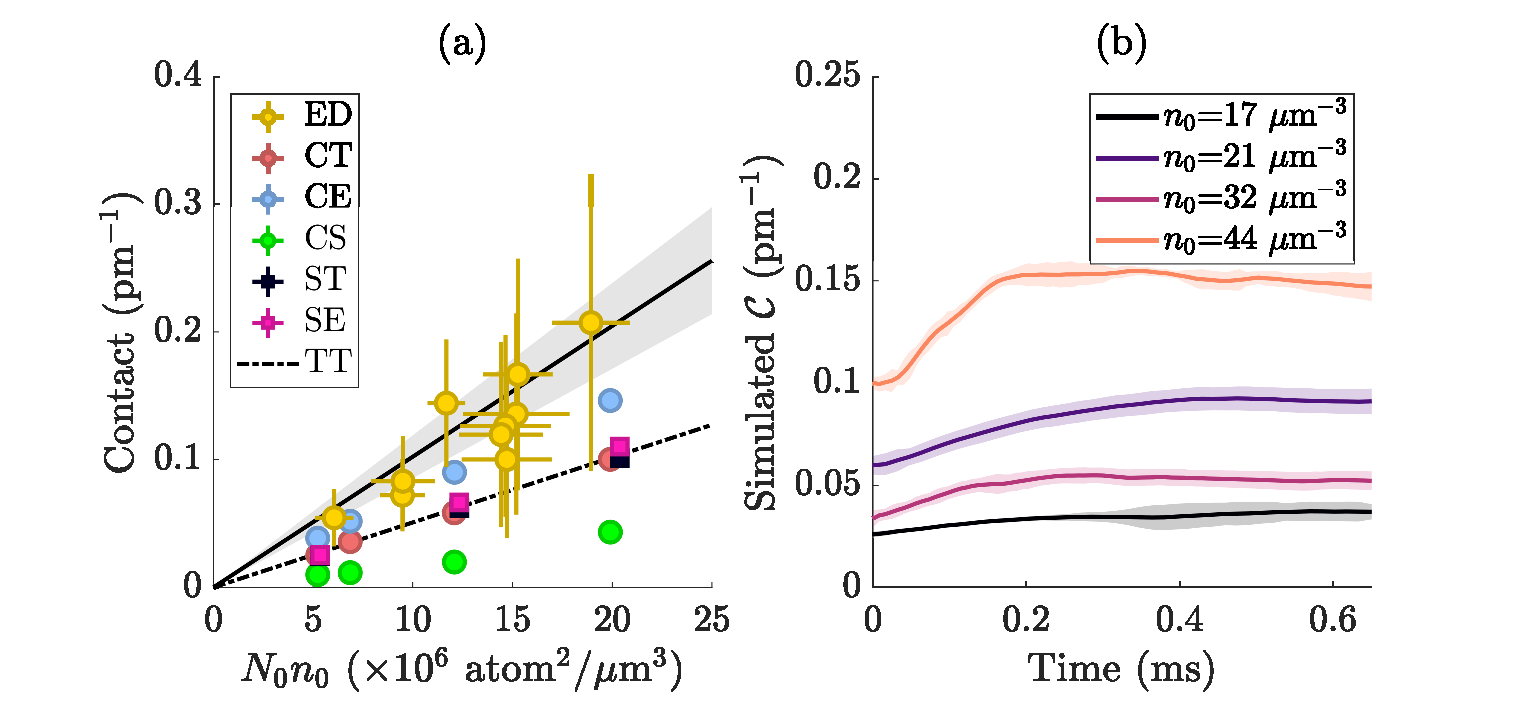
\includegraphics[width=0.5\textwidth]{fig/depletion/main/main/contact_plot_with_theory}
% %         \caption{Comparison of simulations and experiments.
% 	(a) The contact from empirical data (ED) exceeds the prediction by the Tan theory (TT), with trend (and 1$\sigma$ confidence interval) shown as a solid line (grey area).
% 	The simulated contact of BECs in a cigar-shaped trap (CT) are consistent with (TT) before release but compare well with our measurements after expansion (CE).
% 	A slow relaxation of the tight axes of the cigar trap (CS) show a reduction in the large-momentum tails.
% 	Simulations of a spherical trap (ST) show a modest increase after expansion (SE).
% 	(b) Simulations of condensates released from a cigar-shaped trap show an increase in contact after the trap release, stabilizing after a time on the order of 100$\mu$s.}
% %         \label{fig:theory_fig}
% % \end{figure}

% % \begin{table*}[!t]
% %     \begin{tabular}{c c c c c c c}
% %     \hline\hline
% %     Peak density ($\micron^{-3}$) & $N_\textrm{tot}$ ($\times10^5$) & Thermal fraction & ROI counts & Expected counts & $C_\textrm{est}$ ($\times10^{11} m^{-1}$) &$C_\textrm{est}/\mathcal{C}$  \\ 
% %     \hline 
% %     16.9(1.8) & 3.5(4) & 0.09 & 5.6(0.1) & 2.8(0.6) & 5.4(2) & 1.9(0.8) \\ 
% %     18.7(1.4) & 5.0(4) & 0.17 & 6.8(0.1) & 3.7(0.8) & 7.2(3) & 1.8(0.7) \\ 
% %     19.3(2.1) & 4.9(6) & 0.08 & 8.1(0.2) & 4.3(0.9) & 8.3(4) & 1.8(0.8) \\ 
% %     20.4(1.0) & 5.7(3) & 0.09 & 14.8(0.1) & 5.5(1.2) & 1.4(5) & 2.6(0.9) \\ 
% %     38.6(2.6) & 3.9(3) & 0.14 & 4.9(0.1) & 1.9(0.4) & 1.6(9) & 2.5(1.3) \\ 
% %     38.6(3.4) & 3.7(4) & 0.09 & 3.5(0.04) & 1.9(0.4) & 1.1(7) & 1.7(1.0) \\ 
% %     38.6(3.5) & 3.8(4) & 0.11 & 3.7(0.1) & 2.4(0.5) & 1.0(6) & 1.5(0.9) \\ 
% %     38.7(3.4) & 3.7(4) & 0.09 & 4.1(0.1) & 2.1(0.4) & 1.2(7) & 1.8(1.0) \\ 
% %     39.0(4.1) & 3.8(5) & 0.10 & 4.3(0.1) & 2.2(0.4) & 1.3(8) & 1.9(1.1) \\ 
% %     41.3(2.2) & 4.5(4) & 0.12 & 6.5(0.2) & 2.6(0.5) & 2.0(1) & 2.4(1.3) \\ 
% %     \hline\hline
% %     \end{tabular}
% %     \caption{Summary of results for each data run.
% 	The peak density is determined from measurements of the condensed number (via the total number $N_\textrm{tot}$ and condensate fraction) and trapping frequencies, which in turn is used to predict the contact $\mathcal{C}$.
% 	The number of atoms detected in the region of interest can be used to determine the empricial contact $C$ from the $k^{-4}$-like tail by inverting Eqn.
% 	\ref{eqn:pred_num}}
% %     \label{tab:results}
% % \end{table*}

% % \section{Simulations} 
% % To gain further insight we performed simulations of the BEC expansion from a harmonic trap using the Positive-P method, including a cigar-shaped trap with parameters matched to the experimental conditions, and a spherically symmetric trap with identical peak density $n_0$.
% 	The results of these simulations are consistent with the adiabatic sweep theorem before release from the trap, and agree well with our experimental data, as shown in Fig.
% 	\ref{fig:theory_fig} (a).
% 	Following release from the trap, the simulated tail amplitude increased and stabilized at a factor of 1.46(5) above the predictions of \ref{eqn:TotalHarmonicContact} in a few hundred microseconds, much smaller than the 2ms delay between the trap release and application of the rf and Stern-Gerlach pulses.
% 	We also investigated the effect of adiabatic expansion on the in-trap contact by simulating a slow decrease of the trapping frequencies by a factor of two, and found that the in-trap contact decreased in these instances.
	


% % \section{Discussion} We interpret our results as an indication that dispersal of the mean-field energy of the condensate into kinetic energy of the depleted atoms is the mechanism responsible for the disagreement between predicted and measured contact.
% 	In detail, following the quench of the condensate into the free particle regime, the condensate expands hydrodynamically.
% 	This adiabatic reduction in density reduces the local contact density, whereby some depleted atoms are absorbed back into the condensate.
% 	However, the quasiparticles with large $k$ (in the particle branch of the Bogolubov dispersion) have sufficient velocity to escape the cloud before reabsorption.
% 	The relevant timescale for hydrodynamic expansion is on the order of millseconds, while the supersonic depleted particles leave the condensate in microseconds.
% 	Moreover, an atom inside the BEC experiences a force given by the gradient of the mean-field potential (and consequently the density) $F = 4\pi\hbar^2a \nabla  n(x)/m$.
% 	This increases the number of depleted particles with enough energy to escape reabsorption into the condensate, and endows the depleted particles with a greater velocity, leading to an increase in the weight of the tails in the far-field, and of particular relevance to lighter atoms because the acceleration scales with $1/m^2$.
% 	This picture is supported also by the simulations, in which we observe a decrease in the total number of depleted particles coincident with an increase in the large-k population.
	


% % \section{Conclusion}
% % In conclusion, our findings suggest that the quantum depletion is indeed visible in the far-field momentum distribution, and that the hydrodynamic approximation does not capture sufficient microscopic information to make detailed predictions about the high-momentum behaviour.
% 	The interplay between coherent absorption of Bogolubov excitations and the dispersal of the chemical potential into kinetic energy, to which Helium is particularly sensitive, result in overpopulation of the $k^{-4}$ tails of the momentum distribution.
	

% % \section{Future work}
% % The growing suite of far-field investigations \cite{cayla20,chang16} supplemented by this work invite complementary studies of the quantum depletion and contact in situ with ultracold \mhe.
% 	Measurements of the structure factor via Bragg spectroscopy may greatly benefit from the single-particle detection afforded by metastable Helium, which is compelling in light of complications of radio spectroscopy of Helium (discussed in the supplementary material).
% 	An intriguing goal for future studies in Helium is the resolution of particle pairs with opposite momenta in the depleted fraction.
% 	 Such an observation would be challenging because the correlation peak height decreases with the collection efficiency and is broadened by the expnsion dynamics.
% 	Nonetheless, insight into pairing mechanisms in a cold bosonic gas would bear fruit for wider coherent phenomena in condensed matter.


% %     % Leo 2001: The M pairings (1,1),(1,0),(-1,-1), and (-1,0) the collision is dominated by a $^5\Sigma_g ^+$ potential, hence \emph{inelastic processes can occur only via the weak relativistic spin-dipole interaction}.
% 	The scatteering lengths are then almost identical to $a_5$ but with small imag part.
% 	Ilastic rates for (0,0) and (1,-1) from which ionization can occur, are much larger and dominate the total ionization rate for an unpolarized gas.
	
% %     % Ergo - could use RF spectroscopy by modulating the ion production rate via the (1,-1) channel?
% %     % Vassen: $a_{1,-1} \approx 60a_0, a_{1,1} \approx 140 a_0$.
% 	But the chemical potential for each species is different - does this shift the RF resonance? Or affect the ion production rate?
% %     % -> Ion production rate in terms of scattering lengths, spin pol etc?
% %     % -> Find ion production rate from majorana flips: Majorana flip rate x 
% %     % I wonder if contact measurements could just be extracted from the data that Vassen took in 2016?



% % \section{Appendices}
% % \section{Detection}
% %     We use a Roentdek DLD80 multichannel plate and delay-line detector stack \cite{Manning10} with a quantum efficiency of $\sim8\%$, and space and time resolutions of 100 $\mu$m and 3 $\mu$s, respectively \cite{Henson18}.
% 	After the atoms are released from the trap, they fall 859mm to the detector stack, which registers the arrival times and positions $(t_i,x_i,y_i)$ of each atom, indexed by $i$.
% 	The centre of mass of the cloud arrives after a $\tau = 417$ms time of flight.
% 	The velocity of each atom relative to the centre of mass of the cloud is $(v_x,v_y,v_z) = t_{i}^{-1}(x_i,y_i,g_0(\tau^2-t_{i}^{2}))$, where $g_0$ is the local gravitational acceleration.
% 	The velocity conversion carries a negligible error of a few ppm.
% 	We then centre the counts from each realization and detection sequence (termed a \emph{shot}) and transform the counts from cartesian velocity space to spherical polar coordinates with radius $k$ (in $m^{-1}$), polar angle $\theta$ and elevation angle $\phi$, relative to the centre of the cloud, where the velocity-to-wavevector transformation follows from  $\textbf{p}=m\textbf{v}=\hbar\textbf{k}$.
	

% %     The solid angle in k-space available to detect the depleted tails is limited by the 40mm radius of the circular detection surface.
% 	The field of view of our detector is $|k_{x,y}|\approx5\times 10^6$ m$^{-1}$ in the XY plane, which is only just sufficient to reach past the edge of the thermal region.
% 	We sample data from the segments of the sphere with elevation angle $|\phi|>\pi/3$ rad and $|k|<10^7$ m$^{-1}$, centred on the BEC, which encompasses a total solid angle of $0.22\times 4\pi$ steradians.
% 	The detector's dark count rate of $0.56$ Hz cm$^{-2}$ sets the noise floor and contributes an average of 0.4(2) counts to the region of interest per shot.
% 	The distribution of the number of counts in each shot are shown in Fig.
% 	\ref{fig:num_counts}


% % \begin{figure}[!h]
% %     \centering
% %     \includegraphics[width=0.7\textwidth]{fig/depletion/main/som/counts_per_run}
% %     \caption{Number of counts detected in the region of interest across in the depletion measurement (a), the spin mixing calibration (b), and the dark count calibration (c).
% 	An average of 3.0(5) counts were detected in the ROI in the spin-mixing calibration shot, and the background count rate was 0.4(2) counts per shot.}
% %     \label{fig:num_counts}
% % \end{figure}

% % % \todo{Density plots out to larger $|k|$ to show descent into noise floor? How far could we push it until we hit dark counts?}

% % % \section{Spin mixing}
% % % Also lets us determine thermal fraction - note it isn't determinable from the PAL because of the mean-field broadening (but one could just make fits and subtract the thermal part, yes?).
% 	I think the mean-field expansion is particularly bad for Helium, and wasn't reported much before, because we are 5% the mass of popular species like Rb so much more subject to mean-field acceleration!

% % \section{Trap configuration and calibration}

% %     We prepared our BECs with a standard sequence, achieving condensation via forced evaporative cooling in a harmonic magnetic trap with trap frequencies $\sim(425,425,45)$ Hz and a DC bias stabilized by our auxiliary field compensation coils \cite{Dedman07}.
% 	For the tight trap we increased the coil current after the cooling sequence to obtain trapping frequencies $\sim(902,895,71)$ Hz, using a sigmoid step function which to minimize in-trap oscillations.
% 	The trap remained on for 150ms before switching the trap off with a $1/e$ time of $\approx38\mu$s.
% 	The condensates were allowed to expand for 2ms before we transferred some of the condensate into the magnetically insensitive $m_J=0$ state to prevent distortion by stray magnetic fields.
% 	The rf RF sweep generated by a RIGOL function generator, amplified, and applied to the experiment chamber by a coiled antenna inserted into the BiQUIC coil housing.
% 	The pulse swept from 1.6-2.6MHz over 1ms and was centred on the fine structure resonance between the $m_J$ states and transfers atoms into the $m_J = j$ states with efficiencies $\eta_j$.
% 	The sweep was $10^6$-fold wider than the Doppler broadening of the BEC which ensures uniform transfer at all momenta.
% 	Immediately after the RF sweep, the bias coils are switched off and auxiliary push coils in the vertical (Z) and weak horizontal (X) axis are activated using a fast MOSFET switch to implement a Stern-Gerlach separation of the $m_J = -1,~0,$ and $+1$ pulses

% % \subsection{Determining transfer efficiency}

% %     To calibrate the transfer efficiencies, we applied the Stern-Gerlach field for a shorter time, resolving each cloud on the detector.
% 	While the efficiencies $\eta_J$ cannot be calculated by counting the atoms in each cloud because the detector saturates, we can compare the thermal parts.
% 	We align each cloud along the time axis and compute the pointwise proportion of the atomic flux accounted for by each cloud, as depicted in Fig.
% 	\ref{fig:frac_cal}.
% 	The flux fraction of each cloud is roughly constant in the thermal part, indicating the absence of important saturation effects and a spin transfer that is independent of $k$.
% 	The fraction of the total flux of each pulse is identified with the fraction of the original cloud which has been transferred into the respective spin state.
% 	We find these efficiencies are approximately 74\%, 24\%, and 2\% in all runs for the $m_J=+1$, 0, and -1, respectively.
	 
    
% % \begin{figure}[!h]
% %     \begin{center}
% %         \includegraphics[width=0.7\textwidth]{fig/depletion/main/som/frac_cal_profile}
% %         \caption{Determining the rf transfer efficiency.
% 	The time-of-flight profiles of each pulse are aligned with respect their centre-of-mass (a).
% 	The pointwise fraction ((b), dotted line) is uniform where saturation is not evident (solid lines).
% 	Detector saturation is apparent in the peaks of the $m_J=+1$ and $m_J=0$ pulses, but not in the $m_J=-1$ pulse.}
% %         \label{fig:frac_cal}
% %     \end{center}
% %     \end{figure}


% % \subsection{Determination of thermal fraction}
% %     While the $m_J=0$ and $m_J=1$ clouds clearly saturate the detector, the small fraction ($\sim2\%$) in the atoms to the $m_J=-1$ state  does not.
% 	We fit the density outside the condensate with a Gaussian distribution plus constant background and obtain an estimate of the thermal atom number.
% 	Subtracting the number of thermal atoms from the total number in the $m_J=-1$ cloud, minus background counts, yields a estimate of the thermal and condensed fraction, as illustrated in Fig.
% 	\ref{fig:thermal_frac}.

% %     \begin{figure}[!h]
% %     \begin{center}
% %         \includegraphics[width=0.7\textwidth]{fig/depletion/main/som/m1_frac_anal}
% %         \caption{Comparison of thermal fits in the unsaturated $m_J=-1$ pulse including 138 shots.
% 	The weak (X) and strong horizontal (Y) trapping axes are shown in (a) and (b), respectively.
% 	Both projections display a bimodal peak, with the condensate (dotted lines) and thermal parts (thick solid lines) easily distinguished.
% 	Fitting a Gaussian profile (thin solid line) to the velocity distribution of the thermal part yields the thermal number and temperature.
% 	Subtracting the fit leaves the condensate profile (c) which can be yields the condensed number.}
% %         \label{fig:thermal_frac}
% %     \end{center}
% %     \end{figure}



% % \subsection{Analysis of spin transfer measurements}

% %     In early tests of our measurement sequence we noticed a contamination of the signal by spurious counts from the $m_J=+1$ cloud.
% 	We calibrate for this contamination by running the depletion measurement without the RF transfer.
% 	While the cause of the cross-contamination is unclear, we observe that the count density outside the region of interest is similar in both the shots with the RF pulse and those without.
% 	We infer that the remnant counts may be atoms transferred into the $m_J=0$ state by a side effect of the finite switching time of the magnetic fields.
	

% %     % \begin{figure}[!h]
% %     % \begin{center}
% %     %   \includegraphics[width=\textwidth]{fig/depletion/main/som/profile_overlay}
% %     %   \caption{Comparison of average time-of-flight profiles over a single data run for the quantum depletion measurement shots (blue, 871 shots), transfer efficiency calibration (black, 112 shots), detector dark counts (red, 871 shots), and spurious counts (dot-dash, 895 shots).
% 	The time window bounded by $|k|\leq 10\mu$m is indicated with dotted lines.
% 	Shaded area is the standard error over the entire run.}
% %     %   \label{fig:tof_profile}
% %     % \end{center}
% %     % \end{figure}




% % % Note that the temps disagree between axes, but within axes between clouds they are consistent(....ish).
% 	This means we can use the profile ratio method, which is also consistent with comparing the thermal number from the fits.
% % % Perhaps comment on the thermal-subtracted part; the TF profile should have a sharp cutoff, but the smooth edges are suggestive evidence of this roll-off


% % \subsection{Peak density calibration}

% %     The peak density of the condensate can be written as $n_0 = \mu/g$, where $\mu$ is the mean-field energy in the Thomas-Fermi approximation and $g=4\pi\hbar^2a_{1,1}/m$ is the effective interaction strength, in terms of the atomic mass $m$ and $a=7.512$ nm is the s-wave scattering length between pairs of atoms in the $m_J=1$ state \cite{Moal06}.
% 	The expression for the peak density can can be expanded as
% %     \begin{equation}
% %         n_0 = \frac{1}{8 \pi}\left( (15N_0)^2 \left(\frac{m \bar{\omega}}{\sqrt{a_{1,1}} \hbar}\right)   ^{6}\right)^{1/5}
% %         \label{eqn:n0}
% %     \end{equation}
% %     where $\bar{\omega} = \left(\omega_x\cdot\omega_y\cdot\omega_z\right)^{1/3}$ is the geometric trap frequency and $N_0$ is the number of atoms in the condensate.
% 	We simultaneously determine the total atom number $N$ and trap frequency $\bar{\omega}$ in a single shot using a pulsed atom laser and use the thermal fraction to determine the condensed number $N_0$.
	

% %     The pulsed atom laser consists of a series of Fourier-broadened RF pulses centred on the minimum Zeeman splitting in the trap.
% 	The pulse transfers atoms in the trap to the untrapped $m_J=0$ state with an approximately constant transfer rate across the cloud.
% 	We outcouple approximately 2\% of the atoms per 100$\mu$s pulse for $\sim$200 pulses, which eventually depletes the entire trap.
% 	The atom laser thus prevents the detector from saturating and allows an accurate determination of the atom number, up to a factor of the quantum efficiency.
% 	A typical outcome of this procedure is shown in Fig.
% 	\ref{fig:pal_shot}

% %     \begin{figure}[!h]
% %     \centering
% %         \includegraphics[width=0.7\textwidth]{fig/depletion/main/som/pal_shot}
% %         \caption{A kicked pulsed atom laser with motion sampled at 11ms intervals.
% 	The oscillations in the centre-of-mass position of each pulse are shown along the Y axis over time (a).
% 	The apparent frequency can be determined for each axis (b).
% 	The outcoupling efficiency is fixed throughout the sampling sequence (c), producing a geometric decay of the number of atoms in each pulse.
% 	The straight line on a logarithmic scale shows that detector saturation saturation is negligible and that the BEC population does not affect the transfer rate.}
% %         \label{fig:pal_shot}
% %     \end{figure}
    
% % \subsection{Measuring the trapping frequencies}

% %     To illustrate how we obtain the trapping frequencies, consider an undamped harmonic oscillator in one dimension.
% 	The centre-of-mass momentum $p(t) = A \cos(2\pi f t))$ oscillates at a frequency $f$ Hz, and the centre of mass of a pulse outcoupled at time $t'$ lands on the detector at a position $x'(t+\tau) = p(t')\tau/m$, where $\tau$ is the time of flight of the centre of mass.
% 	Sampling the cloud motion with a sampling period T starting at initial time $t_0$ produces a series of pulses whose centres of mass land at $\{x_n = (A\tau/m) \cos(\omega(t_0+nT))\}$.
% 	The sampling frequency $f_s=1/T$ determines the \emph{Nyquist frequency} $f_N=f_s/2$, which is the maximum frequency that can be reconstructed unambiguously from such a sampling regime.
% 	When $f>f_N$ the signal manifests as a lower-frequency oscillation known as the \emph{alias} of the signal.
% 	The aliased frequency $f_a$ is

% %     \begin{equation}
% %      f_a =
% %       \begin{cases}
% %        \frac{Z_n f_s}{2} - f & \text{if } Z_n \text{ even} \\
% %        f - \frac{(Z_n-1)f_s}{2}       & \text{if } Z_n \text{ odd},
% %       \end{cases}
% %       \label{eqn:Z_N}
% %     \end{equation}
    
% %     where $Z_n = \lceil{f/f_N}\rceil$ is the Nyquist zone number, as described in numerous rf engineering references.
% 	While it is not possible to determine $Z_N$ for a signal with an unknown (not necessarily stationary) $f$ from samples taken at a fixed $f_s$, one can vary $f_s$ and determine both $Z_N$ and $f$ from the gradient $d f_a / d f_s$.
	
% % \begin{figure}[!h]
% %     \centering
% %         \includegraphics[width=0.7\textwidth]{fig/depletion/main/som/sawtooth_plot}
% %         \caption{Aliasing of the trap frequency oscillations under different sampling regimes.
% 	The fitted oscillation frequency is shown in each axis for a range of sampling frequencies.
% 	The sawtooth function is a one-parameter fit which determines the underlying frequency of the centre-of-mass oscillations.}
% %         \label{fig:sawtooth_plot}
% %     \end{figure}    

% %     We induce oscillations of the BEC in all three axes by briefly displacing the trap centre with a perturbation to the trapping field.
% 	The maximum sampling frequency is limited by the temporal width of the BEC pulse landing on the detector to about 100Hz, yielding a Nyquist frequency too low to resolve the un-aliased oscillations.
% 	We fit the apparent oscillation frequency in each axis as a function of sampling frequency as shown in Fig.
% 	\ref{fig:sawtooth_plot}, along with a one-parameter fit of Eqn.
% 	\ref{eqn:Z_N}.
% 	We thys determine that the frequencies $(\omega_x,\omega_y,\omega_z)$ of each of the traps used in the experiment are $2\pi\times(45,425,425)$ and $2\pi\times(72,889,893)$, respectively, which are stable to within 5\% throughout the duration of the data collection and to better than $1\%$ in a given run.


% %     \section{Theory}

% % In the Thomas-Fermi approximation, the energy per particle of $N_0$ condensed bosonic atoms is
% % \begin{equation}
% % \frac{E}{N_0} = \frac{5}{7} \mu = \frac{5}{7} \frac{\hbar \bar{\omega}}{2} \left(\frac{15 N_0 a}{a_\textrm{HO}}\right)^{2/5},
% % \end{equation}
% % in terms of the chemical potential $\mu$, where $a_\textrm{HO} = \sqrt{\hbar/(m \bar{\omega})}$ is the harmonic oscillator length \cite{PethickSmith}.
% 	Via the sweep theorem it follows that
% % \begin{equation}
% % \mathcal{C} = \frac{8\pi}{7} \left(15^{2}(a N_0)^{7} \left(\frac{m \bar{\omega}}{\hbar}\right)^{6}\right)^{1/5}.
% % \label{eqn:TotalHarmonicContact}
% % \end{equation}

% % Which by substitution of Eqn \ref{eqn:n0} leads to the expression
% % \begin{equation}
% % \mathcal{C} = \frac{64\pi^2a_{1,1}^{2}}{7}\frac{n_0N_0}{k^4}.
	
% % \label{eqn:TotalHarmonicContact}
% % \end{equation}

% % The Lee-Huang-Yang (LHY) correction to the condensate energy is negligible in our experiments.
% 	The LHY correction for the chemical potential of a uniform condensate with density yields an estimate of the worst-case contribution
% % $$
% % \frac{\partial E}{\partial a_{1,1}} = \mathcal{C}_0\left(1+\frac{64\sqrt{na_{1,1}^{3}}}{3\sqrt{\pi}}\right),
% % $$
% % Where $\mathcal{C}_0$ is the contact computed neglecting the LHY term, and the second term in brackets is the LHY correction which amounts to at most a correction of order 1\%, using the highest $n_0$ observed in our experiments.
% 	In reality the correction will be smaller as the density is not uniform and is bounded above by $n_0$.

% % \subsection{Radio spectroscopic prospects}
% % The basic principle of rf contact spectroscopy is to apply an rf tone which is detuned from the resonance between two spin states, whereby atoms in the initial spin state are coupled to an untrapped channel, thus enabling a differential measurement of the atom number.
% 	The signal strength scales with the difference of reciprocal scattering lengths $\Gamma\propto(1/a_\textrm{i,i}-1/a_\textrm{i,f})$ between initial-initial and initial-final spin states \cite{braaten10,wild12}, which can be manipulated via Feshbach resonance to obtain a good signal.
% 	For He$*$ (spin 1) however, the scattering lengths $a_{1,1}$ and $a_{1,0}$ are identical \cite{Leo01}, rendering the preferred $m_J=1-m_J=0$ transition unusuable.
% 	On the other hand, $a_{1,-1} = 3/7 a_{1,1}$ \cite{vassen16}, and the singlet transition can be driven without populating the $m_J=0$ state.
% 	In principle this could produce a detectable flux of atoms to perform sensitive in-trap contact measurements, however, collisions in the $^1\Sigma_{g}^{+}$ channel have large Penning ionization rates which lead to significant trap losses \cite{Leo01}.
% 	 The ionization products would be detectable by in-vacuum channel electron multipliers but require theoretical work to disentangle from the spectroscopic signal.
% 	Further, such an experiment could not take advantage of a Feschach resonance to increase signal strength or decrease the ionization rate, but it is not \emph{prima facie} impossible.

% % \section{Theoretical methods}
% % To fill in with details of how the P+ simulations were done by Piotr

% % \section{Old material}


% % \subsection{Detection of ultradilute momentum spectra}
% % \label{ssec:qd-model}

% %     Our experiments start with a condensate of helium atoms in the $m_J = +1$ state of the metastable $2^3 S_1$ manifold in a BiQUIC magnetic trap \cite{Dall2007}.
% 	The strongest signal of the depleted tails could be obtained by releasing the BEC from the trap and examining the tails of the detected flux on the detector.
% 	However, the presence of stray DC and transient fields in the chamber would distort the BEC profile and thus also the depletion, in ways that may not be feasible to characterize.
% 	For instance, it is known that our freefall zone contains what is colloquially known as a 'magnetic aperture', which deflects atoms from their freefall trajectory if their transverse momentum is great enough.
% 	This effect is visible in NONEXISTANT FIGURE, which shows the distortion of a thermal cloud, which would otherwise be isotropic.
% 	Indeed, this feature proved problematic in determining the detected count rate from the depleted fraction, because .
% 	Following the method described by Chang \emph{et al} \cite{Chang16}, substantial distortions to the condensate can be avoided by transferring part of the sample to the $m_J=0$ state, which is insensitive to stray magnetic fields.
	

% %     Since for these experiments a precise knowledge of the total atom number and trap frequency is important, we measure the trapped population and trapping frequency at regular intervals throughout each experimental run, using a procedure that avoids detector saturation to measure the atom number and precise determination of the trap frequency.
% 	We identified a contamination of the depletion signal by stray counts attributable to the $m=+1$ state, and calibrate for this by including shots without the RF transfer step.
% 	We also apply corrections for the detector dark count rate and an increased background rate on the leading edge of the condensate, which is attributed to a steady-state leakage of atoms from the trap, due to Majorana flips, Penning ionization, or other collisional effects driving loss.
	

% %     A magnetic field gradient is switched on 5ms after the state transfer pulse, which ensures the magnetically sensitive $M_J = \pm 1$ states are deflected enough to miss the detector.

% %     Since for these experiments a precise knowledge of the total atom number and trap frequency is important, we developed an experimental procedure to regularly calibrate the trapped population and trapping frequency at regular intervals throughout each experimental run, using a procedure that avoids detector saturation to measure the atom number (see supplementary material).
% 	We varied total atom number between 1 and $5\times 10^5$ atoms per condensate by varying the endpoint of the evaporative cooling ramp.

% %     We use two trap configurations with characteristic frequencies $\sim 2\pi\cdot (312,312,52)$ and $2\pi\cdot 666,666,69)$ Hz, which were calibrated on setup by the pulsed atom laser method described earlier in chapter XXX.
	

% %     As in previous chapters, data acquisition shots are interleaved with calibration measurements to predict the key variables 

% %     The trap is switched off in $\sim 100\mu s$ and the atoms allowed to fall 848mm, where they are detected with a multi-channel plate and delay line detector \cite{Manning2010}.
% 	To avoid distortion of the condensate by stray magnetic fields, we transferred approximately 25 - of the condensate into the magnetically insensitive $M_J=0$ state by applying a chirped sine wave 2ms after trap switch-off, swept from 1.6 to 2.6 MHz in 1ms, while a DC magnetic field remained on to preserve the Zeeman splitting between $M_J = {0,\pm 1}$ states.
% 	A magnetic field gradient is switched on after the state transfer pulse, which ensures the magnetically sensitive $M_J = \pm 1$ states are deflected enough to miss the detector.
	

% %     After release from the trap the atoms expand ballistically into the far-field regime, where their position on the detector corresponds to their momentum at trap release.
% 	Therefore we can reconstruct the far-field momentum distribution $n^*(\textbf{k})$ from our detector data.
% 	The observed momentum profile $n^*(\textbf{k})$ cannot be identified completely with the in-trap momentum distribution $n_0(\textbf{k})$ as repulsive interatomic forces distort the profile immediately after release from the trap.
% 	Structure is visible over five orders of magnitude in density, comprised of the condensed, thermal, and depleted fraction before the signal drops below the dark-count background noise.
% 	There is some saturation evident around the low momentum values due to the high atom flux during BEC impact.
% 	Our analysis does not include this part of the momentum profile, and we find evidence that saturation is only an issue during the peak flux, not in the thermal or depleted fractions.

% % The count density from the falling BECs depend explicitly on the trapped population and on the trapping frequencies, necessitating regular calibration of the peak condensate density.
% 	The correction from the detected $m_J=0$ counts to the full condensate profile also requires a measurement of the transfer efficiency of the RF pulse, and a diagnostic of any other sources of detection events, such as detector dark count rate or remnant atoms from the $mJ=\pm 1$ condensates.
% 	In the remainder of this section, I describe the means by which the relevant parameters are calibrated and how they are combined into a model of the detector flux which includes the Tan contact as a free parameter.
% 	In the next section, I describe the algorithm I designed to transform the atomic detection events into an appropriate format to correspond with the model and determine the Tan contact.

% % \subsubsection{Contributions to the model}
    
    
% % \subsubsection{Depletion}
% %     In an ideal world, the experimental procedure is trivial: Form a BEC in a desired trapping configuration, and then release the trap instantaneously and fit the atomic density profile obtained from the DLD image.
% 	Unfortunately, nature intervenes: Because our condensates are formed in a weak-field-seeking state, they are subject to deflection during freefall by stray DC and transient magnetic fields.
% 	These distortions to the BEC profile may be significant at large momenta, although we did not characterize this.
% 	A second potential issue is detector saturation, whereby the trailing side of the BEC is detected with a lower quantum efficiency because of a depletion of charge carriers in the MCP, artificially attenuating the depletion signal.
% 	Both of these issues are ameliorated by transferring a fraction of the condensate into the magnetically insensitive $m_J=0$ shortly after the trap release.
% 	This is achieved by sweeping an RF pulse from 1.6MHz to 2.6MHz, as in \cite{Chang16}, with a DC bias field held on by the Nuller coils.
% 	This field is close to uniform over the scale of the BEC and its freefall path, so by the time the condensate is split into the three spin states, distortions to the cloud would be minimal.

% %     The detection sequence therefore proceeeds with a standard BEC production sequence (as described in INTRODUCTION), with a modified end sequence, pictures in figure QD-SEQUENCE.
% 	The DC bias field is ramped on over 300ms in an exponential ramp with time constant 40ms.
% 	This ensures that no centre-of-mass oscillations are induced in the BEC because of sudden displacements of the trap centre.
% 	The BEC is held for XXX ms to damp out any residual oscillations and is then released.
% 	After 2ms of freefall, the RF chirp is generated by a RIGOL function generator, amplified, and applied to the experiment chamber by a coiled antenna inserted into the BiQUIC coil housing.
% 	The nuller coils are switched off, and the auxiliary push coils in the vertical (Z) and weak horizontal (X?) axis are activated via fast MOSFET switch.
% 	The pulse timing and duration of the push coils required some finessing to minimize the scatter of atoms from a \emph{magnetic aperture} inside the freefall path, as described in later in this section.
% 	The push coils remove the $m_J=\pm 1$ atoms from the detector, so the detector signal is dominated by the undistorted $m_J=0$ cloud.
% 	The cloud then falls freely under gravity through the vacuum chamber, completing the 848mm fall in 417ms.
	

% %     It is important to align the condensates carefully in order to faithfully extract the large-momentum tails.
% 	With an ideal detector, one could simply take the mean of all detected counts.
% 	Because of detector saturation, however, the mean position is heavily biased toward the leading edge of the BEC, and indeed the median (which is robust to outliers) is biased also (it is less robust to skewness).
% 	A workaround can be found in the threefold reflection symmetry of the condensate: The parabolic profile in each principal axis means that if one can identify the edges of the condensate, the centre of mass is at the midpoint along each axis.
% 	This is the basis of the following centering algorithm: For each axis, the atomic detection events are compiled into a histogram as a discrete approximation to the continuous atomic flux.
% 	The region where atomic flux exceeds the background rate by a factor of X is determined to be the BEC region - the extremal positions (or times) with flux above the threshold determine the edges of the condensate, and the mean of these two values determines the centre.
% 	The stages of this algorithm are depicted in figure CENTERING, along with the variation of the BEC centre over the course of a run.
	 

% %     We are concerned with the momentum-space distribution of counts.
% 	The atomic wavevector is related to the in-trap velocity by $\textbf{p}=\hbar\textbf{k} = m\textbf{v}$.
% 	The tranformation from $\textbf{r}-\textbf{r}_0$, where $\textbf{r}_0$ is the centre-of-mass position, is simply a linear transformation $\textbf{v} = \frac{\textbf{r}-\textbf{r}_0}{t_{tof}}$ in the $x$ and $y$ directions.
% 	For $z$, corrections must be made for gravitational acceleration instead given by solving the ballistic trajectories $v_z=-h/t_{tof}-\frac{1}{2}g*t_{tof}$ where $h$ is the fall distance and $g$ is the acceleration under gravity.
% 	\todo{txy-to-vel vs linear error?}

% %     The centred velocity-space counts are then transformed into spherical polar coordinates.
% 	The algorithm is described here is also used for the spin-mixing and dark count calibrations, where the spherical coordinate system is centred at the mean BEC centre-of-mass position in TXY coordinates.
	
% %     \begin{equation}
% %     	(r_i,\theta_i,\phi_i) = (\sqrt{x_{i}^{2}+y_{i}^{2}+z_{i}^{2}},\tan^{-1}(y_i/x_i),\tan^{-1}(z_i/\sqrt{x_{i}^{2}+y_{i}^{2}})
% %     \end{equation}

% %     The counts for each BEC are then compiled into a spherical histogram
% %     \begin{equation}
% %     	N(R(n),\Theta(l),\Phi(m)) = |\{(r_i,\theta_i,\phi_i:r(n)\geq r_i<r(n+1),\theta(l)\geq \theta_i<\theta(l+1),\phi(m)\geq \phi_i<\phi(m+1)\}
% %     \end{equation}
% %     Where $n,l,m$ are indices of the histogram with edges $r(n)$.
% 	Ergh, get this notation sorted out.
	
% %     The memory demands can get exhaustive - holding large TXY datasets and also lots of large 3D histograms - can reduce the by lots of writing to disk, but the cheater way around this was to compute the mean by adding to the histogram by looping over each shot, and ditto the squared number of counts to find the variance later.
% 	There would also be a biasing effect by including the empty bins which are defined outside the detector area.
% 	These are found by a messy case analysis in \verb|find_final_bin_idx.m| (hyperlink to dox html?).
% 	 These are excluded from subsequent sums over profiles.
% 	The bins are normalized by the spherical volume element
% %     % \begin{equation}
% %     \begin{align}
% %     	V(n,l,m) &= \int_{R(n)}^{R(n+1)} d r \int_{\Theta(l)}^{\Theta(l+1)} d \theta \int_{\Phi(m)}^{\Phi(m+1)} d \phi r^2 \sin(\phi)\\
% %     	&= (\Theta(l+1)-\Theta(l))(Cos(\Phi(n)+\frac{pi}{2})-Cos(\Phi(n+1)+\frac{pi}{2}))(\frac{r(n+1)^3-r(n+1)^3}{3})
% %     \end{align}
% %     % \end{equation}
% %     \todo{CHECK THIS 3.}

    

% % \subsubsection{Flux model}

% %     The pointwise density of atom detection events in momentum space can be described by the expression
% %     \begin{equation} 
% %     n(\textbf{k}) = \sum_{m=-1}^{1} n_m(N,\omega_{x,y,z},T,\textbf{k}) + \delta(\textbf{k}) + \lambda(N,\bar{\omega},\textbf{k})\Theta(-\theta)
% %     \end{equation}
% %     The first terms $n_m$ refer to the detected density of atoms from the $m_J=m$ condensates, which depends on the momentum vector  on the total atom number N, the temperature T , and harmonic trapping frequencies $\omega_{x,y,z}$.
% 	The dark count rate $\delta$ is momentum-dependent due to its non-uniformity on the detector.
% 	While the BEC is held in the magnetic trap, it is subject to loss mechanisms such as Majorana transitions, Penning ionization, or three-body recombination, and so `leaks' at a rate rate $\lambda$, which may also manifest a momentum-dependence because of its spatial non-uniformity on the face of the detector.
% 	 When the trapped gas is released, the leak stops, hence the Heaviside theta function $\Theta(-\theta)$ ensures this term only contributes on the lower side of the falling BEC.
% 	The distortion-free depletion signal is found in the contribution $n_{0}(\textbf{k},N,\omega_{x,y,z},T)$.
% 	The calibration protocol described in this section is designed to extract this by subtracting away the various sources of background counts, and also ensure accurate calibration of the experimental parameters $N$, $T$, and $\omega_{x,y,z}$


% %     \begin{figure}
% %     \includegraphics[width=\textwidth]{fig/depletion/main/partition_QD_files_profile_overlay_st.eps}
% %     \label{fig:qd-tof1}
% %     \end{figure}
% %     \begin{figure}
% %     \includegraphics[width=\textwidth]{fig/depletion/main/partition_QD_files_profile_overlay_hf.eps}
% %     \end{figure}

% % \subsubsection{Peak density}
% %     The peak density of the condensate can be derived from the expression for the chemical potential $\mu = g \rho(0)$: (see \cite{PitaevskiiStringariBook16}, pp.181)
% %     % \begin{equation}
% %     \begin{align}
% %     \rho_0 &= \frac{\mu}{U}\\
% %         &= \frac{\hbar\bar{\omega}}{2}\left(\frac{15N_0a_0}{\bar{a}}\right)^{2/5} / 4\pi\hbar^2a_0/m
% %     \end{align}
% %     % \end{equation}
% %     % NB: The N a_0/a_h0 is discussed in \cite{Dalfovo99} and is what determines the interaction/kinetic energy ratio
% %     % for fun: calculate the total energy of the condensate (sum over kinetic energies) - and for different segments?
% %     % what is the healing length 1/sqrt(8 pi n a) and corresponding k scale
% %     Where $N_0$ is the total condensed number, $\bar{\omega} = \left(\omega_x\cdot\omega_y\cdot\omega_z\right)^{1/3}$ is the geometric trap frequency, $a_0=7.512$ nm is the interatomic scattering length \cite{Moal06}, $m$ is the atomic mass, and $\bar{a} = \sqrt{\frac{\hbar}{m\bar{\omega}}}$ is the harmonic oscillator length .
% 	Thus the peak density of the condensate can be determined by a measurement of the trapping frequencies and the total condensate number.
% 	Fortunately, these parameters can be measured simultaneously with the pulsed atom laser method described in chapter TUNEOUT.
% 	As shown in chapter TUNEOUT, the trap frequency is stable to XXX accuracy.
% 	Therefore, even over runs of several hours, the trap frequency variation contributes only YYY much variation in peak density.
% 	The variation in atom number can be as much as XXX per cent, which corresponds to a YYY per cent variation in peak density.
	

% %     \begin{figure}
% %     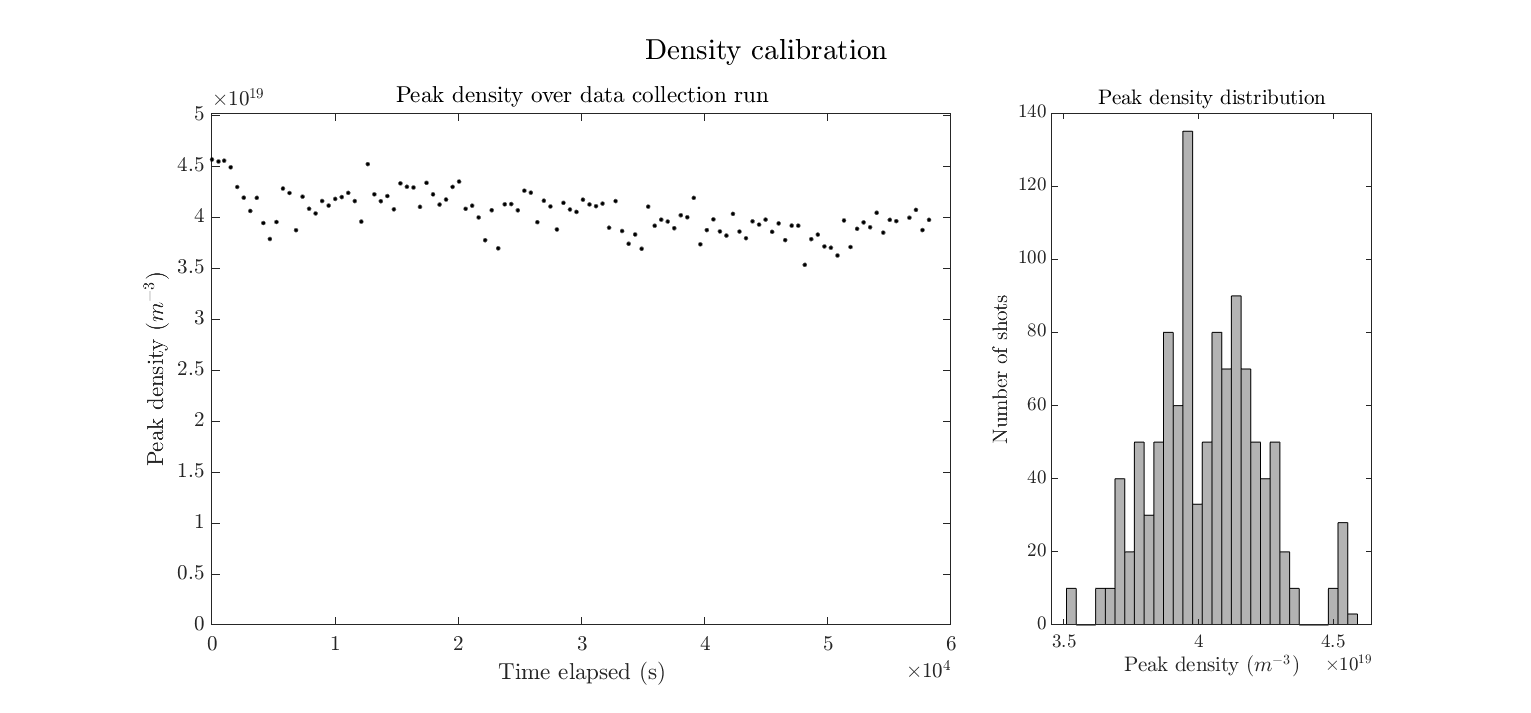
\includegraphics[width=\textwidth]{fig/depletion/main/calibrate_QD_shots_01_stats.eps}
% %     \label{fig:qd-n0_by_time}
% %     \caption
% %     \title
% %     \end{figure}


% % \subsubsection{Dark counts}
% %     Even when the Helium source is not active, the MCP-DLD detector stack stil registers detection events.
% 	These may be genuine, spontaneous electron detection events seeded by background gas in the chamber or thermal excitation in the MCP, or indeed by transients in the DLD lines that are sufficient to trigger a digital pulse from the discriminator.
% 	These are referred to as \emph{dark counts}, by analogy to the Poissonian electronic noise in digital camera sensors like CMOS arrays.
% 	Indeed, the detector dark counts are uncorrelated events and so form a Poisson distribution \todo{Clarify \& graph of dark count statistics}.
% 	The correction for detector dark counts is entirely analogous to \emph{darkfielding} in precision photography, where images are taken without a light source to correct for detector noise.
% 	The spatial distribution of dark counts is shown in figure FIGURE, the time profile in figure PROFILES, and the calibration procedure is described in the next section.

    
% %     % average dark count rate of 5.6228 kHz/m$^2$.
% 	The evident structure in the dark count rate is accounted for in 

% %     The dark count rate is assumed to be uniform in time.
% 	It may be altered by high atomic fluxes of the condensate itself, but this is not a concern for the following reasons: One, we observe very similar thermal tails both above and below the condensate, suggesting that, at least, the quantum efficiency and dark count rates are not significantly different.
% 	Two, although there are some temporary hotspots on the detector during the peak BEC flux, these are only observed co-temporally with the falling BEC.
% 	The quantum depletion is detected far beyond the regions where this effect is noticable, and so they are not expected to contaminate the signal.

% %     A second source of background counts is the so-called \emph{trap leakage}, which is a measurable increase in the steady-state count rate while a BEC is held in the trap, which is visible in figure \ref{fig:qd-tof1}.
% 	Unlike the dark counts, the trap leakage has no obvious spatial structure.
% 	Correcting for these counts is therefore a matter of computing an average spurious count rate and then subtracting this from the detected count density, as described in the next section.
% 	Because the trap leakage stops when the trap is released, this correction is applied only to the leading side of the condensate.
    
% %     The best way to deal with it would be to extend the hold for ages, and then get heaps of statistics, but in the end I wound up using the 20-odd ms window of hold before drop in each case.
% 	This still gets to within ??? some margin of error when using all the data I have for a given run.
% 	In reality, the leak rate should depend on the BEC number, as, for instance, Majorana losses would induce an exponential decay of the trapped atom number, and Penning ionization losses scale with the squared density.
% 	There would also be density-dependent collision effects feeding the trap leak rate driven by changing the trapping frequencies, and different trap configurations would change the trap centre position, which could affect the detected density of the trap leakage.
% 	However, the count rates are so low that we do have the sensitivity to these effects, and so take a relatively simplistic treatment of the trap leakage, described in the next section.

% % \subsubsection{Transfer efficiency}

% %     The efficiency $\eta_0$ of the population transfer to the $m_J=0$ state is critical in determining the Tan contact, as the factor $1/\eta_0$ is the correction applied to the final signal in order to estimate the true signal density in the original condensate.
	

% %     The RF chirp transfers atoms into the $m_J = m$ states with efficiencies $\eta_m$.
% 	The chirp was adopted because, as described in \cite{Chang16}, it would minimize the momentum-dependence of the spin transfer pulse.
% 	The transfer efficiency cannot be calculated by counting the detected number in each cloud, as the condensates still saturate, leading to incorrect estimates.
% 	This is illustrated in figure SATCH-FRACTION.

% %     Instead, we can take advantage of the fact that the condensates have identical spatial profiles (to within a good approximation), albeit with different amplitudes, c.f.
% 	hydrodynamic expansion - density-dependent effects v small after 2ms?


% %     The momentum distribution of the thermal fraction of a degenerate Bose gas is known to be isotropic (see \cite{PitaevskiiStringariBook16} pp.
% 	160) and constitutes less than 5\% of the total population throughout this experiment.
% 	The momentum distribution of the thermal fraction takes the form

% %     \begin{equation}
% %         n_T(\textbf{k}) = \frac{1}{\lambda_T m \bar{\omega}}g_{3/2}\left(e^{-\beta (\hbar) k^2/2m}\right),
% %     \end{equation}

% %     which is manifestly invariant under rotations about the centre of momentum.
% 	Therefore, integrating over the $k_x$ and $k_y$ directions resolves the $k_z$-dependence of the momentum distribution.
% 	(You can talk through the physics better than this matey).
% 	After centering the clouds using a thresholding procedure described in the \textbf{Depletion} section, the time-of-flight profile of each cloud is divided pointwise by the sum of all the time-of-flight profiles.
% 	In the regions where the detector is unsaturated, the ratios $n_m(\textbf{k})/n(\textbf{k})$, where $n_m(\textbf{k})$ and $n(\textbf{k})$ are the momentum-space density of the $m_J=m$ clouds and the original BEC, respectively, are estimates of the transfer efficiency $\eta_m$, as shown in figure \href{fig:qd-fraction_calibration}.
% 	This figure also shows that detector saturation is not apparent in the thermal fraction of the trailing side of the BEC, and therefore suggests that saturation would be negligible in the depleted wings in the trailing edge.
% 	Further, the uniformity of the determined ratio across the thermal fraction is evidence that the RF transfer efficiency is independent of the particle momentum.

% %     \begin{figure}
% %     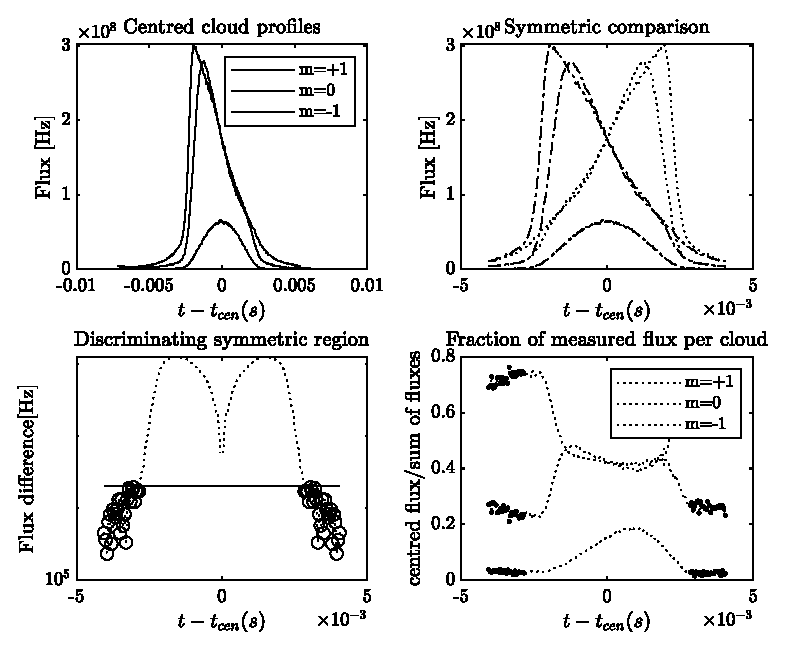
\includegraphics[width=\textwidth]{fig/depletion/main/frac_cal.eps}
% %     \label{fig:qd-fraction_calibration}
% %     \caption
% %     \title
% %     \end{figure}

    

% % \subsubsection{Spin-mixing}

% %     In the depletion detection shots, we have observed a remaining presence of $mJ=1$ atoms.
% 	These are visible in figure PROFILES, as the step-up in flux rate at 0.56s in a) and the peak in detector flux at 0.55s in b).
% 	The cause of which is unclear but is suspected to be due to a collision process with a feature inside the chamber, as illustrated in figure CLOUDSMASH.
% 	Regardless of the cause, we calibrate for this contamination (also called \textit{spin mixing}).
% 	by running the depletion measurement without the RF transfer, instead measuring the time-of-flight profile of the $m_J=1$ cloud.
% 	After subtracting the background rates as appropriate, this provides a suitable calibration image for the spurious counts, which is subtracted from the measurement profiles, weighted by the transfer efficiency $\eta_1$.

% %     The count density of the $mJ=1$ states depends on the trapping frequencies, as shown by the clear difference between their contributions to figure PROFILES a) and b).
% 	This is likely because the trap centre and BEC width shifts with changing trap frequencies, so the push coil sequence would, left unchanged, result in different spray patterns on the detector.
% 	Unfortunately, we cannot rule out the presence of $mJ=-1$ counts on the detector without additional calibration (for example, taking yet another shot with a different RF transfer fraction).
% 	However, as the $m_J=-1$ clouds are determined to have about one tenth of the total atom population, and the $m_J=+1$ counts are suppressed by nearly three orders of magnitude by the push coils, if we assume a similar suppression of the $m_J=-1$ cloud then \todo{Worst-case bias of -1 counts}


    


% % \section{Determination of the Tan constant}\label{ssec:qd-processing}


% % 	The fit to the depletion profile $\tilde{n_0(k)}$ is obtained by taking the weighted sum of the k-space images for the depletion, spin-mixing, and dark count rates:

% % 	\begin{equation}
% % 		\tilde{n}_0(k) \approx \frac{1}{\eta_0}\left(n_0(k) - \eta_1(n_1(k)-\delta(k))-\delta_k-\lambda(k)\right)
% % 	\end{equation}

% % 	To avoid detector hotspots and to ensure we only use angular bins which extend far enough in k-space to capture some depletion, we specify the spherical sample region $\{(r_k,\theta,\phi): 1E6<r_k<3E7,\theta_{range},\phi_{range}\}$.
% 	Averaging over the angular bins commutes with the image summation because they're all linear.
% 	This produces one-dimensional radial profiles, as shown in figure K-PROFILES.
% 	The depletion and the thermal tails are isotropic, but the BEC is not, so the BEC peak is not physically representative.
% 	Or, remove it from the plot so it's just thermal - i.e.
% 	plot from the largest TF momentum.
	
    

% %     As in \cite{Chang16} we find the large-$\textbf{k}$ momentum distribution is isotropic, unlike the in-trap mean-field interactions, and conclude that the extreme momenta are not strongly affected by the mean-field.
% %     A typical condensate profile shown in Fig.
% 	\ref{k_profile}.
% 	Structure is visible over five orders of magnitude in density, comprised of the condensed, thermal, and depleted fraction before the signal drops below the dark-count background noise.
% 	There is some saturation evident around the low momentum values due to the high atom flux during BEC impact, however this part of the histogram is not used for the analysis.

% %     The Tan contact parameter is extracted by a fit to BEC density profile after subtracting the calibrated noise profiles.
% 	The functional form
% % 	$$
% %     n_{fit}(k) = \frac{N_{th}g_{3/2}exp(-k^2 \lambda_{dB} ^2 /4\pi)}{1.202(2\pi/\lambda_{dB})^3} + \frac{C}{(2\pi)^3 k^4} + const,
% %     $$

% %     includes contributions from the thermal fraction and depleted fraction and includes the free parameters $N_{th}$ the number of thermal atoms, $\lambda_{dB} = h/\sqrt{2\pi m k_B T}$ the thermal de Brogliewavelength, $const$ a constant to account for the detector background count rate, and $C$ is the scale of the fitted power law assumed to correspond to the Tan contact parameter.
% 	In the local density approximation, $C \approx C_{LDA} = \int d\textbf{r} [16\pi^2 \rho^2(\textbf{r},t)a^2]$, where $a$ is the scattering length and $\rho$ the atomic density.
% 	The initial guess for the fit constant $C$ is set to Tan constant predicted by the peak density and number calibrations.
% 	The initial temperatures are set manually for each directory.
% 	The thermal and the depleted parts of the profile are fitted individually to better constrain fitting parameters, and then a joint function is fitted to find the best overall parametrization.
	
    
% %     We verified the fitting method by analysing a test data set of known parameters, which was generated by the Metropolis-Hastings algorithm, and find the method recovers the test set parameters within a factor less than our experimental uncertainties.
    
% % \subsection{Verifying the method}
    
% %     Reliably estimating the parameters of a power-law distribution is nontrivial\cite{Clauset09}, and the robustness of the fitting method above has not been exhaustively tested.
% 	The LDA prediction is essentially that the single-particle wavefunctions, hence the single-particle probability distribution over momentum, are affected by many-body effects.
% 	One computes the single-particle probability density by dividing the condensate density by the number of particles (hence the $N_0$ term in the LDA), and then the problem of extracting the contact parameter from the data is an exercise in statistical parameter estimation.
% 	As shown by Clauset et al \cite{Clauset09}, fitting these functions tends to produce incorrect estimates of parameters.
% 	The method outlined in Clauset was proven to asymptotically converge with probability 1 to the correct fit parameters of a power law distribution, but would need to be extended to derive a maximum likelihood estimator for a power law overlaid on a constant background.

% % \section{Discussion}
% % \label{qd-discussion}

% % \subsection{Findings}
    
% %     According to theoretical predictions based on the local density approximation \cite{Chang16}, the contact constant $C_{LDA}$ of the depleted fraction should vary linearly with the peak condensate density $n_0$.
% 	This was found in previous experiments\cite{Chang16}, although their scaling factor greater by a factor of $\sim$6.5.
% 	In Fig.
% 	XX, we plot our measured values of $C$ and $n_0$ , identifying the fit parameter $C$ with the contact constant $C_{LDA}$ .
% 	A linear fit to the contact constant variation finds a gradient approximately 1.7 times more than the theory predicts.

% %     Our findings suggests that the visibility of the quantum depletion in the far-field momentum distribution is indeed a real physical effect.
% 	Our findings are corroborated by theoretical work.
% 	However, the question remains open as to why the observed population of the quantum depletion is greater than predicted by the otherwise successful Bogoliubov theory.
% 	Possible confounding factors:
% %     \begin{itemize}
% %     	\item Intra-cloud scattering
% %     	\item Trap switchoff or early-falltime dynamics,switch-off timescale may be relevant (compare \cite{Chang16} with \cite{Qu16}).
% %     	\item $m_J=-1$ counts
% %     \end{itemize}

% % 	We have assumed that the RF transfer is momentum-independent, but this could be violated by inhomogeneities or transients in the magnetic field.
% 	The RF pulse may increase the Penning ionization rate in the depolarized sample, even though the density is low, which would alter the momentum profile.
% 	While applying the magnetic separation pulse, the condensates may scatter off each other.


    


% % \subsection{Future work}
	
% %     A possible future experimental extension is to outcouple atoms using a broadened Raman transition.
% 	This would have the benefit of moving the outcoupled atoms through the cloud rapidly, minimising the effects of repulsive inter-atomic interactions that normally affect the outcoupled profiles.
% 	This should shed some light on whether interactions during trap switch off are the origin of the momentum tails.
% 	One could test the importance of particle scattering or Penning ionization by delaying the Rabi transfer to the $M_J = 0$ state, but this could increase vulnerability to stray magnetic fields.
% 	There is scope to optimize the RF transfer sequence to achieve much higher transfer efficiency for a stronger signal
    
    

    

